\documentclass[mathserif,hyperref,UTF8,openany,b5paper]{ctexbook}
\usepackage{amsmath}
\usepackage{amsfonts}
\usepackage{tikz}
\usepackage{caption}
\usepackage{wrapfig}
\usepackage{listings}
\newtheorem{exmp}{例}[section]
\setlength{\parskip}{0.15em}
\usepackage[most]{tcolorbox}
\newtheorem{defn}{定义}[section]
\newtheorem{thm}{定理}[section]
\newtheorem{pro}{命题}[section]
\newtheorem{cor}{推论}[section]
\newtheorem{lam}{引理}[section]
\newtheorem{kuo}{扩展}[section]
\usepackage{booktabs}
\tcolorboxenvironment{align}{boxrule=0pt,boxsep=0pt, colback={white!90!yellow},
enhanced jigsaw,breakable,left=3mm,
before skip=5pt,after skip=5pt,
borderline west={1mm}{0pt}{yellow}}
\tcolorboxenvironment{equation}{boxrule=0pt,boxsep=0pt, colback={white!90!yellow},
enhanced jigsaw,breakable,left=3mm,
before skip=5pt,after skip=5pt,
borderline west={1mm}{0pt}{yellow}}
\tcolorboxenvironment{defn}{boxrule=0pt,boxsep=0pt, colback={white!90!red},
enhanced jigsaw,breakable,left=3mm,
before skip=10pt,after skip=10pt,
borderline west={1mm}{0pt}{red}}
\tcolorboxenvironment{lam}{boxrule=0pt,boxsep=0pt, colback={white!90!orange},
enhanced jigsaw,breakable,left=3mm,
before skip=10pt,after skip=10pt,
borderline west={1mm}{0pt}{orange}}
\tcolorboxenvironment{pro}{boxrule=0pt,boxsep=0pt, colback={white!90!violet},
enhanced jigsaw,breakable,left=3mm,
before skip=10pt,after skip=10pt,
borderline west={1mm}{0pt}{violet}}
\tcolorboxenvironment{cor}{boxrule=0pt,boxsep=0pt, colback={white!90!green},
enhanced jigsaw,breakable,left=3mm,
before skip=10pt,after skip=10pt,
borderline west={1mm}{0pt}{green}}
\tcolorboxenvironment{thm}{boxrule=0pt,boxsep=0pt, colback={white!90!blue},
enhanced jigsaw,breakable,left=3mm,
before skip=10pt,after skip=10pt,
borderline west={1mm}{0pt}{blue}}
\tcolorboxenvironment{exmp}{boxrule=0pt,boxsep=0pt, colback={white!90!cyan},
enhanced jigsaw,breakable,left=3mm,
before skip=10pt,after skip=10pt,
borderline west={1mm}{0pt}{cyan}}
\tcolorboxenvironment{kuo}{boxrule=0pt,boxsep=0pt, colback={white!90!orange},
enhanced jigsaw,breakable,left=3mm,
before skip=10pt,after skip=10pt,
borderline west={1mm}{0pt}{orange}}
\usepackage{pgfplots}
\pgfplotsset{compat=1.15}
\usepackage{mathrsfs}
\usetikzlibrary{arrows}
\pagestyle{empty}
\usepackage{siunitx} 
\usepackage{bm}
\usepackage{tabu}
\usepackage[hidelinks]{hyperref}
\usepackage{fancyhdr}
\pagestyle{fancy}
\fancyhead[RE]{\leftmark \quad \thepage}
\fancyhead[LO]{\thepage \quad \leftmark }
\fancyhead[RO,LE]{RQLuo}
\fancyfoot[LE,RO]{讨论交流群:\textbf{153815103}}
\fancyfoot[C]{}
\fancyfoot[RE]{数学物理笔记 \quad \thepage}
\fancyfoot[LO]{\thepage \quad 数学物理笔记}
\renewcommand{\footrulewidth}{1pt}
\renewcommand{\headrulewidth}{1pt}
\usepackage{color}
\definecolor{dkgreen}{rgb}{0,0.6,0}
\definecolor{gray}{rgb}{0.5,0.5,0.5}
\definecolor{mauve}{rgb}{0.58,0,0.82}
\lstset{frame=tb,
  language=Python,
  aboveskip=3mm,
  belowskip=3mm,
  showstringspaces=false,
  columns=flexible,
  basicstyle={\small\ttfamily},
  numbers=none,
  numberstyle=\tiny\color{mauve},
  keywordstyle=\color{blue},
  commentstyle=\color{gray},
  stringstyle=\color{dkgreen},
  breaklines=true,
  breakatwhitespace=true,
  tabsize=3
}
\usepackage{xeCJK}
\usepackage{graphicx}
\usepackage{background}
\backgroundsetup{contents=
\includegraphics{art.png}, scale=1.3, opacity=0,angle=0}
\setCJKmainfont{MSimSun.ttf}[BoldFont = HSimSun.ttf, ItalicFont=fzkaiti.ttf]
\usepackage{imakeidx}
\makeindex
\begin{document}
\thispagestyle{empty}
\newpage 
\
\newpage
\thispagestyle{empty}
\section{序言}
\textbf{给刚刚踏上追寻智慧和真理之路的初学者。愿你们不忘初心,永远秉持着一颗热衷于刨根问底的内心。}

宏伟华丽的建筑总是需要有个深入地底稳固无比的地基,我们对智慧和学问的追寻亦是如此。如果我们一味的追求处在高出的上层建筑,满足于现代理论的华丽结论,和有趣的实验与运用,那么我们总会意识到自己大多的理解都是无法深入且似懂非懂的,甚至于还会有一些难以察觉的谬误。最为严重的是,我们将必然慢慢地看不见脚下的路,在黑暗中迷茫失去了方向和理想。不过对于物理学来说,我并不是极端地声张一开始就一定要去深究其根基和原理,因为以往的物理学大厦本就是从上层探索发现建立而成的,并且根基需要太多的耐心去钻研而又缺乏显而易见的趣味和成果。当然,如果你本就热衷于探究苦涩艰难的抽象原理的话,那么从根基出发坚持不懈说不定将会开出一番新天地,毕竟谁也不知道将来的物理学将会如何的修建。

Hassani的数学物理,在我打开这本书的一开始,从它的序言和目录结构读起,就已经让我不由的期待万分和激动不已,因为这就是我一直以来所梦寐以求的大而全的教材,它能够让我完整的建立和巩固我的物理学在数学上的框架和根基。不但能够扫除我长久依赖的一些似是而非的困惑,或许还能给予我一些可遇不可求的灵感。不过,这本书像是一本没有什么废话的百科全书,使得其中的内容太密集根本就难以读下去。因此,我便从最为简单和基础的集合开始研读,对每一个知识点我都一点一点细致的剖析,思考,和举例。很多时候,我还会在原来的基础上进行一些拓展和深入,或者补充说明和更加详细的解释。自然而又慢慢地也就有了这本数学物理笔记,不单单是为了督促和勉励自己,得以坚持下来深入地思考和研读完整本书。此外,另一个目的是为了和大家一起分享我对物理数学的热爱和一些微不足道的见解,希望能够给大家追寻梦想带来一些的帮助,最好我希望还能遇到一些志同道合的爱好者一起加入到对物理数学的探究和讨论中。我想大概许多和我一样热爱物理数学但是天赋平平的朋友们面对这样一本枯燥乏味庞大全面的书籍都会感到望而生畏吧。所以,我在记笔记的同时不仅写的能够让我自己看懂和学习,我也尽可能的写的通俗易懂,给出一些例子和插图,将一些难点和令人疑惑的地方做好充分的解释试图让所有的爱好者都能够从中更加容易的理解和掌握更多深刻的思想。

\begin{wrapfigure}{r}{4cm}
\centering

\includegraphics[scale=0.4]{qq.png}
\end{wrapfigure}
\thispagestyle{empty}
不过由于作者本身也未曾尽管专业的训练,水平十分的有限,不免会出现一些谬误或者解释不清楚的地方,恳请发现纰漏的朋友能够之处遗漏所在,我的邮箱是1084172661@qq.com。或者如果可以我恳请所有正在使用或者阅读这本笔记的朋友能够加入QQ群:153815103。这样我们就能够一起学习,讨论,和思考,我也十分的欢迎各种提议和批评。

此外,我也由衷的期望着能够有越来越多的人开始思考和研究数学物理建筑结构这样一门纯粹艺术。毕竟,这个世界实在有着太多美丽,巧妙,神奇,和崇高之处了,以至于我们的理论作为其倒影都是那样的优雅。甚至于有时,数学的理论实在过于的完美和纯粹,以至于我差点忘记了它不过人为一厢情愿的“虚假的完美”创造。因此,无论在这笔记中我是多么的偏向于探讨数学理论,而将物理学搁置一旁,都请牢记我们身处于眼前的世界中,所探究物理学中数学基础最终目的,归根结底是为了更好的领悟大自然运行规律的玄妙与其鬼斧神工的创造。

\thispagestyle{empty}
最后,我想分享一段一直以来对我的人生有着深远影响的一段话与君共勉,出自\textbf{《小逻辑》,[德]黑格尔著,贺麟译:} \textit{ “不去认识真理,只去认识那表面的有时间性的偶然的东西,只去认识虚浮的东西,这种虚浮习气在哲学里已经广泛地造成,在我们的时代里更为流行,甚至还加以大吹大擂。但我要特别呼吁青年的精神,因为青春是生命中最美好的一段时间,尚没有受到迫切需要的狭隘目的系统的束缚,而且还有从事于无关自己利益的科学工作的自由。同样青年人也还没有受过虚妄性的否定精神,和一种仅只是批判劳作的无内容的哲学的沾染。一个有健全心情的青年还有勇气去追求真理。”}
\thispagestyle{empty}
\tableofcontents
\thispagestyle{empty}
\chapter{预备(Preliminaries)}
\section{集合(sets)}
\thispagestyle{fancy}
集合论是近代数学的基石,但是这也并不意味着集合是一个十分抽象和深奥的概念。计算机科学中集合本质上是一种数据结构,我认为这是一个十分优雅和直观的理解。关于集合的最为基础部分的讨论在这里将会比较的紧凑,因为这个部分理应对大家来说是复习,当然如果你已经生疏或者初学,那么你还是需要多看几遍牢记一些基本概念和符号的。
\begin{defn}
集合(set)是将事物或者对象聚集在一起的方式,满足:\\
\textbf{1.无序性}:集合的每个元素之间没有次序之分同时也没有权重差异。\\
\textbf{2.互异性}:集合的每个元素都是唯一的,任意两个元素都是不同的。\\
\textbf{3.确定性}:元素要么属于集合要么不属于,不允许摸棱两可的存在。\\
我们将集合$A$中的每一个成员$a$称之为该集合的元素(elements)。\index{元素(elements)}\index{集合(sets)}
\end{defn}
比如学校里所有的学生就构成了一个集合。学校里面的任意一个学生也就是该集合的元素。有时,为了表示几何涵义也将$a$称之为一个\textbf{点(point)}。
\begin{defn}
$a$ 是集合$A$中的一个元素写做,$a\in A$。$a$ 不是集合$A$中的一个元素写做$a\notin A$。
\end{defn}
\begin{defn}
集合通常是由可枚举的元素在一对花括号里面来表示。如果一个集合只有一个元素,那么我们称其为\textbf{单元素集合(Singleton)}。
\end{defn}
\begin{exmp}
$ \{3,1,4,2\} $ 是由四个数组成的集合;$\{a\}$是单元数集合。
\end{exmp}
此外,$ \{\cdots,-4,-2,0,2,4,\cdots\} $ 这样一个集合或许你能够一眼就看出这是所有偶数的集合。注意我们之前已经明确了集合是无序的,这里为了让大家能够明白我所想要表达的特点所以是按照顺序书写的。不过这样的符号表述有着明显的缺陷,那就是无法严格和清晰的表达该集合中元素的特点。
\begin{defn}
很多情况下我们会使用$\{n|P\} $来标记和定义一个集合。这样的符号我们可以将其读作“对于该集合中的每一个元素$n$都符合该数学真命题性条件$P$。”或者“集合中的所有元素都是在条件为真的情况下成立的”。
\end{defn}
\begin{exmp}
运用我们所学过的符号我们就能够将之前的偶数集合表示写成一个更加严谨的形式,$ Even \equiv \{n|n = 2a \land a\in \mathbb{Z}\} $ 。不过,这样的写法虽然规范和严格,但是有些的累赘。因此,大多数情况下我们会将其简化为: 
\begin{equation}
    Even \equiv \{2n|n\in \mathbb{Z}\}
\end{equation}
\end{exmp}
\begin{defn}
如果集合$A$中的所有元素都同样是集合$B$中的元素,那么我们称集合$A$是集合$B$的\textbf{子集(Subset)}\index{子集(Subset)}。符号上我们将其记作$A \subseteq B$或者$B \supseteq A$。上述定义写做符号形式为,$(\forall a\in A \implies a \in B) \iff A \subseteq B $。如果$A$不是$B$的子集我们就写做,$C \not \subseteq B$。如果$A$是$B$的子集并且$A \neq B$,那么$A$是$B$的\textbf{真子集(proper subset)}\index{真子集(proper subset)}。
\end{defn}
如果一个事物它不是其自身,则违背了基本逻辑,因此它不可能存在。
\begin{defn}
\textbf{空集(empty set)}\index{空集(empty set)}指的就是一个不存在任何元素的集合,定义为:$\{a|a\neq a\}$。
类似的,我们还可以定义\textbf{零}为:若事物$A$等价于非$A$,也就是$A\Leftrightarrow\neg A$,则$A$为零(不存在)。
\end{defn}
\begin{cor}
空集是任意集合的子集。
\end{cor}
这里我和你或许都就会有些疑惑,之前我们对子集的定义似乎并不支持这一推论。那么,我们可以试着换个更加完善的说法:
\begin{thm}
$A$是$B$的\textbf{子集}当且仅当$A$中没有任何不属于$B$的元素。
\end{thm}
\begin{figure}
  \begin{minipage}[t]{0.5\linewidth}
\centering 
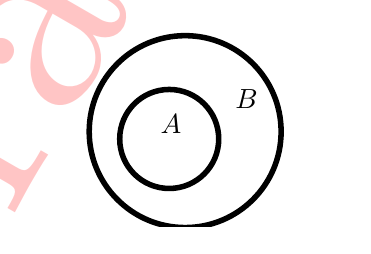
\begin{tikzpicture}[line cap=round,line join=round,>=triangle 45,x=1cm,y=1.2cm]
\clip(-2,-1) rectangle (2,1.1);
\draw [line width=2pt] (0,0) circle (1.2186272121823938cm);
\draw [line width=2pt] (-0.20240368224310518,-0.07780899272326403) circle (0.6287800263654525cm);
\draw (-0.43701824783886994,0.2878617051790603) node[anchor=north west] {$A$};
\draw (0.5131571554096853,0.5530269339926106) node[anchor=north west] {$B$};
\end{tikzpicture}
\caption{A是B的子集}
  \end{minipage}%
  \begin{minipage}[t]{0.5\linewidth}
\centering 
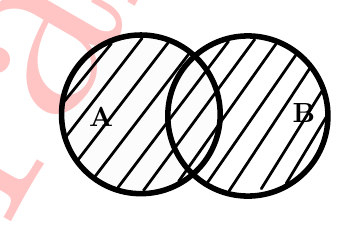
\begin{tikzpicture}[line cap=round,line join=round,>=triangle 45,x=1cm,y=0.96cm]
\clip(-1.3,-0.8) rectangle (2.6,1.6);
\draw [line width=2pt,fill=black,fill opacity=0.01] (0.13750641459048774,0.45358997318752925) circle (1.0076012169321562cm);
\draw (1.9405831373969709,0.7307179396494703) node[anchor=north west] {$\mathbf{B}$};
\draw [line width=2pt] (1.496478212259932,0.4314928707864001) circle (1.0170069851331778cm);
\draw (-0.6451208270385644,0.6691535595438624) node[anchor=north west] {$\mathbf{A}$};
\draw [line width=1pt] (0.1537034172083272,1.4610609998028656)-- (-0.8219464111476876,0.14583928261772283);
\draw [line width=1pt] (0.4828849744524474,1.400148932128197)-- (-0.665502292031316,-0.15504557412526132);
\draw [line width=1pt] (0.748806203547108,1.2545723577533532)-- (-0.44479415163766045,-0.3687154827919019);
\draw [line width=1pt] (-0.23755592494535832,1.3887843133249467)-- (-0.8603966974028738,0.5930517652207836);
\draw [line width=1pt] (1.2501305232557693,1.41821270130162)-- (-0.1511329974961343,-0.5117843076763496);
\draw [line width=1pt] (1.5832791520639606,1.4447888811697496)-- (0.17194228908653608,-0.5534226299664009);
\draw [line width=1pt] (1.8526936681410067,1.3840755479336984)-- (0.6173638981040444,-0.4324105955928744);
\draw [line width=1pt] (2.1089791598384973,1.2433708154462089)-- (0.9848069273806597,-0.4474244768861044);
\draw [line width=1pt] (2.2880075026049473,1.0700730069757372)-- (1.2599486506532311,-0.557626421460909);
\draw [line width=1pt] (2.4506270016080896,0.7834918702098659)-- (1.6675419704144852,-0.5304551019168232);
\draw [line width=1pt] (2.513215406860833,0.454916895307528)-- (1.9833598145149725,-0.46139542748793627);
\end{tikzpicture}
\caption{并集}
  \end{minipage}
\end{figure}
\begin{defn}
有限集合$A$中的所有子集构成的集合我们将其称之为\textbf{幂集合(Power Set)}\index{幂集合(Power Set)},记作$2^A$。
\end{defn}
\begin{pro}
集合A的子集数是$2^N$,其中$N$是A集合中元素的个数。
\end{pro}
\begin{kuo}
为什么集合A的子集数目是$2^N$?每当我看到这样的问题,我总是会回想起抛掷三枚硬币会带来8种组合的例子,我们同样可以把这个思想转化到处理集合$\{a,b,c\}$的所有子集。各硬币在每个事件中有正反两个状态,正如各元素在每个集合中有存在或不存在两个状态。比如空集就是当所有不存在,对应三个硬币全是反面。子集$\{b,c\}$就是当$a$不存在但$b,c$存在,对应三个硬币分别为反正正。这样我们就不难看出集合中任意元素对于任意该集合的子集都有两种状态,那么显然总共的子集构成方式就有$2^N$个。
\end{kuo}
两个习题作为回顾中学知识的练习:\textbf{1.}如果集合有$N$个元素,试着推导一个函数$\Omega$来输出由$n$个元素构成子集的所有方式的数目$\Omega(N,n)$。\textbf{2.}由公式推导出 $\sum_{n=0}^{N}\Omega(N,n) = 2^N$。
\begin{figure}
  \begin{minipage}[t]{0.5\linewidth}
    \centering
\centering 
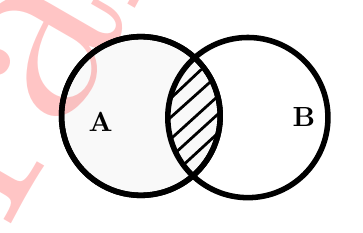
\begin{tikzpicture}[line cap=round,line join=round,>=triangle 45,x=1cm,y=0.9cm]
\clip(-1.3,-0.8) rectangle (2.6,1.7);
\draw [line width=2pt,fill=black,fill opacity=0.01] (0.13750641459048774,0.45358997318752925) circle (1.0076012169321562cm);
\draw [line width=2pt,fill=black,fill opacity=0.01] (0.13750641459048774,0.45358997318752925) circle (1.0076012169321562cm);
\draw (1.9391839469400265,0.711129273252232) node[anchor=north west] {$\mathbf{B}$};
\draw [line width=2pt] (1.496478212259932,0.4314928707864001) circle (1.0170069851331778cm);
\draw (-0.6493183984094004,0.6411697504049502) node[anchor=north west] {$\mathbf{A}$};
\draw [line width=1pt] (0.5163627587232824,0.7029277719106348)-- (0.9032809864742565,1.10845600331842);
\draw [line width=1pt] (0.5233369001122053,0.13602850000529126)-- (1.1077468087719222,0.7254240951476261);
\draw [line width=1pt] (0.48001150180798996,0.3983472171847063)-- (1.0216181229495431,0.9369187427694718);
\draw [line width=1pt] (0.6002151971430794,-0.041914817567480684)-- (1.1436588577707307,0.5076036144792476);
\draw [line width=1pt] (0.7059127623296081,-0.2082801180042647)-- (1.1153401157937135,0.21048204416347943);
\end{tikzpicture}
\caption{交集}
  \end{minipage}%
  \begin{minipage}[t]{0.5\linewidth}
\centering 
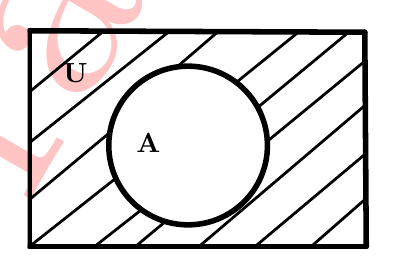
\begin{tikzpicture}[line cap=round,line join=round,>=triangle 45,x=1cm,y=1cm]
\clip(-1.9,-0.9) rectangle (2.5,1.95);
\draw [line width=2pt] (0.13750641459048774,0.45358997318752925) circle (1.0076012169321562cm);
\draw (-1.5743375814958118,1.618048879269928) node[anchor=north west] {$\mathbf{U}$};
\draw (-0.643156141019888,0.7345259607199572) node[anchor=north west] {$\mathbf{A}$};
\draw [line width=2pt] (-1.874029805373916,1.910788175085134)-- (-1.874029805373916,-0.8268258972609867);
\draw [line width=2pt] (-1.874029805373916,-0.8268258972609867)-- (2.4000003279827866,-0.8268258972609867);
\draw [line width=2pt] (2.4000003279827866,-0.8268258972609867)-- (2.3813771030008404,1.8921649501031879);
\draw [line width=2pt] (2.3813771030008404,1.8921649501031879)-- (-1.874029805373916,1.910788175085134);
\draw [line width=1pt] (-0.9365409570227881,1.9066853792498994)-- (-1.874029805373916,1.137014446547303);
\draw [line width=1pt] (-0.10091012842047808,1.9030283515536093)-- (-1.874029805373916,0.4913194595909136);
\draw [line width=1pt] (0.525724384175637,1.9061511221865315)-- (-0.0034700649284603313,1.4512802280189603);
\draw [line width=1pt] (-1.874029805373916,-0.23033964347799207)-- (-0.8564576170352344,0.6188041257214532);
\draw [line width=1pt] (-1.874029805373916,-0.8268258972609867)-- (-0.780195553966079,0.037557150839863496);
\draw [line width=1pt] (0.748806203547108,1.2545723577533532)-- (1.5417408656237315,1.8958395069407243);
\draw [line width=1pt] (2.1589528805947404,1.8776645786443378)-- (1.0216181229495431,0.9369187427694718);
\draw [line width=1pt] (-0.45418342499124054,-0.3619854960971415)-- (-1.0475036046341228,-0.8268258972609867);
\draw [line width=1pt] (1.1436588577707307,0.5076036144792476)-- (2.383883402540101,1.5262452173711667);
\draw [line width=1pt] (2.3877204510002104,0.966036142195195)-- (0.27884100680995805,-0.8268258972609867);
\draw [line width=1pt] (2.391949044108153,0.3486615484355592)-- (0.9910045953648001,-0.8268258972609867);
\draw [line width=1pt] (2.395849790958069,-0.2208474916522033)-- (1.7031681839196422,-0.8268258972609867);
\draw [line width=1pt] (-0.1511329974961343,-0.5117843076763496)-- (-0.5282777268855285,-0.8268258972609867);
\end{tikzpicture}
\caption{补集}\label{补集图}
  \end{minipage}
\end{figure}
集合作为储存和表达数据的结构,和数字一样自然有着一些特定的数学运算和操作。
\begin{defn}
如果一个集合是由分别来自集合$A$或者集合$B$中的所有元素所构成的,那么我们称其为A和B的\textbf{并集(Union)}\index{并集(Union)},记作:
\begin{equation}
    A\cup B\equiv \{c|c\in A \lor c\in B\}.
\end{equation}
\end{defn}
\begin{exmp}
\textbf{并集的例子:}$\{1,4,7\} \cup\{e,d,c,b\} =\{e,d,1,4,7,c,b\}$。
\end{exmp}
\begin{defn}
如果一个集合中的任意元素属于集合$A$并且也属于集合$B$,那么我们称其为A和B的\textbf{交集(Intersection)}\index{交集(Intersection)},记作:
\begin{equation}
    A\cap B\equiv \{c|c\in A \land c\in B\}.
\end{equation}
\end{defn}
\begin{exmp}
\textbf{交集的例子:}$\{e,4,7\} \cap\{e,d,c,b,4\} =\{e,4\}$
\end{exmp}
\begin{defn}
对于三个及以上的集合的并集,也就指的是$A_1\cup A_2 \cup A_3 \cup \cdots \cup A_n$,我们将其记作$ \cup_{i=1}^{n}A_{i} $。同样的对于交集是$ \cap_{i=1}^{n}A_{i}$。
\end{defn}
\begin{defn}
如果一个集合中的任意元素都不属于集合$A$,那么我们称其集合$A$的\textbf{补集(complement)}\index{补集(complement)}为将其记作$\overline{\rm A}$或者:
\begin{equation}
    \sim A\equiv \{c|c\not\in A\}
\end{equation}
\end{defn}
如果我们单单就说一个集合是$A$的补集,那么很显然它将会是一个有无穷多个在$A$集合之外的元素构成的集合,并且这样的集合是无法给我们任何明确的意义的。这就类似于我若告诉你一个事物它不是猫,你还是不能知道我说的究竟是什么。因此,给定集合$A$以外一个范围是很且重要的。
\begin{defn}
我们将集合$D$作为关于$A$的补集的范围,也就是将集合$A$在$D$上的补集定义为:$D\sim A \equiv \{c|c\in D $ and $ c\not \in A\} $。
\end{defn}
\begin{exmp}
你或许已经发现了这样的定义会带来两种不同的案例:\\
\textbf{第一种}:$A$并非$D$的子集$D \sim A\equiv\{e,4,7,a\} \sim \{e,d,c,b,4\} = \{a,7\}$。
\begin{defn}
若$A$并非$D$的子集,则其为$A$在$D$中的相对补集($A,D$的\textbf{差集(difference)}记作$D \sim A$或$D-A$)。\index{差集(difference)}
\end{defn}
\textbf{第二种}如图1.4所示,$A$是$D$的子集:比如,$\mathbb{Z}\sim\mathbb{Z}^-=\mathbb{N}$:
\begin{defn}
如果$A$是$D$的子集,则$D \sim A$称之为$A$在$D$中的绝对补集。$D$是\textbf{全集(Universal Set)}往后都将记作$U$。
\end{defn}
\end{exmp}
\begin{pro}
任意集合都可以是全集。
\end{pro}
不过依据不同特定场合,全集会有着更加清晰明确的使用。比如,在实分析中实数集就是全集,复分析中复数集就是全集。
\begin{thm}\textbf{交集,并集,补集的定理:}\\
\textbf{交换律(Commutative property):} 
\begin{equation}
A\cup B = B\cup A,\ A \cap B = B \cap A.
\end{equation}
\textbf{结合律(Associative property):}
\begin{align}
(A \cup B )\cup C = A \cup (B\cup C ),\\
(A \cap B )\cap C = A \cap (B\cap C ).
\end{align}
\textbf{分配律(Distributive property):}
\begin{align}
(A \cap B )\cup C = (A \cup C) \cap (B\cup C ),\\
(A \cup B )\cap C = (A \cap C) \cup (B\cap C ).
\end{align}
\textbf{德摩根定律(De Morgan's Law):} 
\begin{align}
    A\sim (B\cup C) = (A\sim B)\cap (A\sim C),\\
    A\sim (B\cap C) = (A\sim B)\cup (A\sim C).
\end{align}
\end{thm}
集合中元素的顺序是不重要的。然而,在很多情况下元素的顺序是不得不被考虑的。例如,二维平面的坐标$(x,y)$代表了二维平面上的任意一点,其中$(1,2)\not =(2,1)$。这就引出了下面的定义:
\begin{defn}
\textbf{有序对(Ordered Pairs)}\index{有序对(Ordered Pairs)}的概念,我们将其记作$(a,b)$。如果$a,b$分别属于集合$A,B$中的元素,那么一个由$a,b$的有序对组成的集合就是$A,B$的笛卡儿积,记作:$\boxed{A\times B = \{(a,b)|a \in A \land b \in B\}}$。对于三个及以上的集合的笛卡儿积,我们将其\textbf{广义化定义}记作: $A_1\times A_2 \cdots \times A_n = \{(a_1,\cdots,a_n)|a_i \in A\}$。若集合$A_1=A_2 \cdots = A_n$,我们可以将$A_1\times A_2 \cdots \times A_n $简写为$A^n$。
\end{defn}
比如一副扑克牌的花色和大小的笛卡儿积就构成了52张牌。
\begin{exmp}
关于广义化的例子就是当集合$A=\mathbb{R}$,$A^n$就是$n$维笛卡尔坐标中全部有序对$(x_1,\cdots,x_n)$的\textbf{$n$元组(n-tuples)}\index{$n$元组(n-tuples)}实数集合$\mathbb{R}^n$。\index{笛卡儿积(cartesian product)}
\end{exmp}
\subsection{等价关系(Equivalence Relations)}
在许多情况下,集合中的元素之间往往都有着某些特定的联系,因而它们都能够自然地组合或划分成该集合的多个子集。为了描述两个及以上或同一集合上的元素之间的关系,我们将会定义一种叫做关系的数学结构。
\begin{defn}
若$A,B$为两个非空集合,从$A$到$B$的\textbf{关系(Relations)}\index{关系(Relations)}指的就是对$A \times B$ 中的任意一个有序对$(a,b)$中元素$a$与$b$的一个\textbf{条件比较判断(comparison test)}\index{条件比较判断(comparison test)},如果$a$与$b$满足条件并通过比较判断,那么\textbf{$a$与$b$有关系},记作$a\vartriangleright b$(作为一个存放着所有符合条件的有序对的一个$A \times B$ 的子集)。否则$a$与$b$没有关系。任意$A^n$的子集都可以被当作集合$A$上的\textbf{$n$元关系}。
\end{defn}
\begin{exmp}
设条件为$(a > b) \land (a+b>4)$,
$\{1,3,7\}\times \{1,2,4\} = \{(1, 2), (3, 2), (7, 1), (3, 1), (1, 4), (7, 4), (3, 4), (1, 1), (7, 2)\}$
其中$(7,1)$符合条件,$(7>1)\land (7+1>4)$。同理有,\\
$\{1,3,7\}\vartriangleright \{1,2,4\} = \{(7, 4), (3, 2), (7, 2), (7, 1)\}$
\end{exmp}
\begin{defn}
如果 $\vartriangleright$ 是集合$A$上的一个二元关系且满足以下三个性质,
\begin{itemize}
\item \textbf{自反性(Reflexively):} $a \vartriangleright a, \quad \forall a\in A$
\item \textbf{对称性(Symmetry):} $a \vartriangleright b \implies b \vartriangleright a,\quad \forall a,b\in A$
\item \textbf{传递性(Transitivity):}$a \vartriangleright b \land b \vartriangleright c \implies a \vartriangleright c  ,\quad \forall a,b,c\in A$
\end{itemize}
那么我们就认为它是一个在集合$A$上的\textbf{等价关系}。
\end{defn}

等价关系是一类特殊的二元关系,它是拥有一个等价条件判断的二元关系,因此它也是$A\times A$的子集。另外关于定义中所使用的符号$a\vartriangleright b$我们称之为“$a$(在某种条件或者设定下)等价于$b$”。等价关系是一个十分重要的数学构造,因为它是广义上的对两个事物按照其属性带来的等价性的规范。比如,我们最为熟悉的实数之间的等价也是符合广义等价关系的三个性质的。此外,三角形的全等和相似也是等价关系。

\begin{defn}
如果$ \vartriangleright $是集合$A$上的等价关系并且$a\in A$,对于任意的$b \in A$都有$ b \vartriangleright a$,也就是集合中所有元素都等价于$a$,那么我们称在该条件下构成的集合为元素$a$的\textbf{等价类(Equivalence Classes)}\index{等价类(Equivalence Classes)}, 记作\begin{equation}
    [a]=\{b\in A | b \vartriangleright a\} 
\end{equation}
\end{defn}

写代码的时候有时我们需要把一个大的循环拆分成由多个步骤组成的小周期来处理。毕竟我们常常会希望我们$n$个线程同时处理整个大循环,因此我们自然的就会将大循环按照整数索引的余数$n$划分为$n$个小任务让线程分别处理。这样就自然产生了等价类。

\begin{exmp}
设集合$A=\{0, 1, 2, 3, 4, 5, 6, 7, 8\}$,该集合上的关系条件为$a \equiv b \mod{3} $,这样的条件使其成为等价关系。注意$a和b$是该集合自身的笛卡儿积带来的有序对$(a,b)$。该集合上的等价关系就是:\\$A \vartriangleright A = \{(0, 0), (2, 8), (1, 4), (0, 6), (0, 3), (2, 2), (2, 5), (1, 1), (1, 7)\} $ 。其中有三个等价类分别为$[0]=\{0,3,6\},[1]=\{1,4,7\},[2]=\{2,5,8\}$。
\end{exmp}

\begin{thm}
如果$\vartriangleright$是在集合$A$上的一个等价关系并且有$a,b \in A$, 那么要么有$[a] \cap [b]=\emptyset$或者是$[a]=[b]$。
\end{thm}

这个定理其实挺显然的,毕竟逻辑上一个事物不能同时等价于两个及以上不相同的其他事物,它本质上是因为等价关系的传递性。如果你还不能理解那就再回过头来看看上面的例子。由该定理可得知,如果$b \in [a]$,那么元素$b$绝对不会出现在不等于$[a]$的其他任何等价类中。因此,一个等价类中的任意元素都是该等价类所独属的,并且我们将等价类的任何元素作为该类的\textbf{代表(representative)}\index{代表(representative)}。由于等价关系的对称性,我们将其记作$\bowtie$。

等价关系的概念是自然的存在于物理学中的,因为决定同一物理性质的数学对象应该被认为是等价的。比如,单位长度的\textbf{量子态函数}与幅角不同的单位长度复数的乘积,可以组合在一起,因为它们都代表相同的物理状态。此外,我们知道\textbf{磁场(Magnetic Field)}\index{磁场(Magnetic Field)}是\textbf{螺线矢量场(solenoid vector field)}\index{螺线矢量场(solenoid vector field)}因为其\textbf{散度(divergence)}\index{散度(divergence)}为零, $\mathbf{\nabla} \cdot \mathbf{B} = 0 $。磁场的\textbf{向量势(vector potential)}\index{向量势(vector potential)}$\mathbf{A}$的定义为,$ \mathbf{B} = \mathbf{\nabla} \times \mathbf{A}$。那么,我们就有$\mathbf{\nabla} \cdot \mathbf{B} =\mathbf{\nabla} \cdot (\mathbf{\nabla} \times \mathbf{A}) = 0$。这就说明该向量势在任意\textbf{组成方向(components)}\index{组成方向(components)}上都有连续二阶偏导数。这里我们也就很自然的可以联想到,如果让向量势加上一个有连续二阶偏导数的标量函数$f$,那么它并不会改变原来的磁场。 

所以,螺线向量场也就是磁场所对应的向量势不是唯一的,这就表明不同的向量势可以计算出同一个磁场。也就是说,设$\mathbf{A} = \mathbf{A'} + \mathbf{\nabla} f$,因为$\mathbf{\nabla} \times \mathbf{\nabla} f=0$,所以$\mathbf{B} =\mathbf{\nabla} \times \mathbf{ A' }+ \mathbf{\nabla} \times \mathbf{\nabla} f = \mathbf{B'}$。那么,我们就很自然的联想到了之前讨论过的等价关系和等价类。其中,$\mathbf{A} = \mathbf{A'} + \mathbf{\nabla} f$就是关于$\mathbf{A}     \bowtie\mathbf{A'}$ 的一个等价条件判断。它们之间的等价关系是建立在彼此都可以计算出同一磁场这一条件或者设定下成立的,也就是说等价类$[\mathbf{A}]$是一个包含了所有能够计算出同一磁场的不同向量势。
\begin{defn}
如果集合$A$的子集所构成的一个集合$\{A_1,A_2,\cdots,A_n\}$满足以下三个条件,
\textbf{交集为空(disjoint):} $A_i \cap A_j,\quad \forall i \not = j$,
\textbf{不含空集:}$A_i \not = \emptyset , \quad \forall i$,
\textbf{并集为$A$:}$\cup_{i=1}^{n}A_{i} =A$,
我们就将其称之为集合$A$的\textbf{划分(partition)}\index{划分(partition)}$P$。集合$P$中的每个子集我们称之为\textbf{类(class)}\index{类(class)}。
\end{defn}

划分的定义是十分显然和易懂的,划分集合就像划分蛋糕一样。你应该已经看出来了划分和等价类有着直接显然的联系,那就是对于一个集合$A$上的任意等价关系都可以确定一种划分方式,其所有等价类构成的集合是集合$A$上的一个划分,每一个等价类都是集合$A$的类。反之亦然,给定一个集合上的划分,我们也可以归纳出该集合上的等价关系,因为集合中两个元素等价仅当其存在于同一个划分的区块中。
\begin{defn}
集合$A$的所有等价类所组成的集合$\{[a]|a\in A\}$称为$A$在等价关系上的\textbf{商集(Quotient Set)}\index{商集(Quotient Set)},记作$A/\bowtie$。
\end{defn}
\begin{exmp}
回顾\textbf{例1.3.1},现在我们考虑整数集$\mathbb{Z}$上的\textbf{同余关系(Congruence Relation)}\index{同余关系(Congruence Relation)} $a\vartriangleright b \iff k|a-b$ 。
这里我只不过是换了个表达(因为这样的表达能够更容易的推导出同余关系是等价关系),意思是$a-b$可以被$k$整除,也可以记作$a \equiv b \mod{k} $。当我们从模$3$推广到了模$4$之后,我们可以很轻易的看出整数集$\mathbb{Z}$在同余关系上的\textbf{商集 }为,$\mathbb{Z}/\bowtie = \{[0],[1],\cdots,[k-1]\}$。其中$[0]=\{\cdots,-3k,-2k,-k,0,k,2k,3k,\cdots\}, [k-1] = \{\cdots-2k-1,-k-1,-1,k-1,2k-1,3k-1 \cdots\}$。
\end{exmp}

\begin{defn}
设集合 $\mathbb{R}^n$为是实数集$\mathbb{R}$的\textbf{广义笛卡儿积}。那么,$\mathbb{R}^n$就是由\textbf{$n$元组有序对}构成的$n$维空间。若点$X = (x_1,x_2,\cdots,x_n),Y = (y_1,y_2,\cdots,y_n)$是在原点出发的同一条射线,则它们等价。也就是如果$x_i = k y_i,\forall i$那么$X \bowtie Y$为\textbf{等价关系}。这里面的一个\textbf{等价类}就是一条射线,一个\textbf{射影空间(Projective Space)}\index{射影空间(Projective Space)}$\mathcal{P}^{n-1}$的定义就是 $\mathbb{R}^n$在该等价关系上的商集,$\mathbb{R}^n/\bowtie$。
\end{defn}
\begin{wrapfigure}{l}{2.8cm}
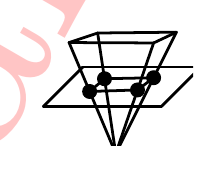
\begin{tikzpicture}[line cap=round,line join=round,>=triangle 45,x=1cm,y=1cm]
\clip(-1.2,-0.5) rectangle (0.9,1);
\draw [line width=1pt] (-0.5,0.5)-- (-1,0);
\draw [line width=1pt] (0.5,0)-- (1,0.5);
\draw [line width=1pt] (-0.5,0.5)-- (1,0.5);
\draw [line width=1pt] (-1,0)-- (0.5,0);
\draw [line width=1pt] (-0.08158233566060395,-0.5976325631830551)-- (-0.6745396353743969,0.81111808576633);
\draw [line width=1pt] (-0.08158233566060395,-0.5976325631830551)-- (-0.31131440051096554,0.9321931640541408);
\draw [line width=1pt] (-0.08158233566060395,-0.5976325631830551)-- (0.6888710288231207,0.9427214317313417);
\draw [line width=1pt] (-0.08158233566060395,-0.5976325631830551)-- (0.39934366770009566,0.8058539519277296);
\draw [line width=1pt] (-0.22410096959690662,0.35142377750874687)-- (-0.41292129872986955,0.18956405193804302);
\draw [line width=1pt] (-0.41292129872986955,0.18956405193804302)-- (0.1948125986733451,0.2089708653524711);
\draw [line width=1pt] (0.1948125986733451,0.2089708653524711)-- (0.39946670283328906,0.36412040247545285);
\draw [line width=1pt] (-0.22410096959690662,0.35142377750874687)-- (0.39946670283328906,0.36412040247545285);
\draw [line width=1pt] (-0.6745396353743969,0.81111808576633)-- (0.39934366770009566,0.8058539519277296);
\draw [line width=1pt] (0.39934366770009566,0.8058539519277296)-- (0.6888710288231207,0.9427214317313417);
\draw [line width=1pt] (0.6888710288231207,0.9427214317313417)-- (-0.31131440051096554,0.9321931640541408);
\draw [line width=1pt] (-0.31131440051096554,0.9321931640541408)-- (-0.6745396353743969,0.81111808576633);
\begin{scriptsize}
\draw [fill=black] (-0.22410096959690662,0.35142377750874687) circle (2.5pt);
\draw [fill=black] (-0.41292129872986955,0.18956405193804302) circle (2.5pt);
\draw [fill=black] (0.1948125986733451,0.2089708653524711) circle (2.5pt);
\draw [fill=black] (0.39946670283328906,0.36412040247545285) circle (2.5pt);
\end{scriptsize}
\end{tikzpicture}
\caption{射影平面}
\end{wrapfigure}
这也类似于绘画中的透视技巧,透视需要先选择透视点(可以在纸外),然后每对本应当平行的线条相交于透视点。这样一张画纸就相当于被三维空间中的一个点上的所有射线所穿过。这些射线所构成的集合就是一个$2$维的射影空间。因此,$n$维度的射影空间应当对应$\mathbb{R}^{n+1}$。
\section{映射(Maps)}
之前我们讨论了集合间元素的关系和分类,接下来我们将要深入的探讨在集合之间的联系。我们所熟悉的函数也可以称作映射就是这样的联系。所谓映射就是一个输入某个事物然后经过“加工”后输出“成品”的“工厂”。我们当然不会满足于这样类比,所以接下来我们将对其给以明确的定义。
\begin{defn}
如果非空集合$X$中的\textbf{任意一个}元素$x$能够按照特定的法则$f$\textbf{唯一}地对应或者联系到集合$Y$上的一个元素$y$,那么我们就称其为\textbf{从集合$X$到集合$Y$的一个映射$f$ (Map)}\index{映射(Maps)},记作$f:X\xrightarrow{}Y$ 或 $X\xrightarrow{f}Y$。对于集合内的元素,我们将元素$y$记作$f(x)$,来表示元素$x$经过映射$f$对应到了的元素$y$,也就是$x\xrightarrow{f}y$。数学上\textbf{函数(Function)}\index{函数(Function)}一般指的是一个陪域为实数集$\mathbb{R}$或复数集$\mathbb{C}$的映射。
\end{defn}
\begin{defn}
\textbf{恒等映射(Identity map)}\index{恒等映射(Identity map)}或者恒等函数是一个特殊的映射$id_A (a):A\xrightarrow{}A$,我们将其定义为,$id_A (a)=a, \forall a \in A$,简单来说,它就是一个输入和输出是完全相等的映射。
\end{defn}
\begin{wrapfigure}{r}{4cm}
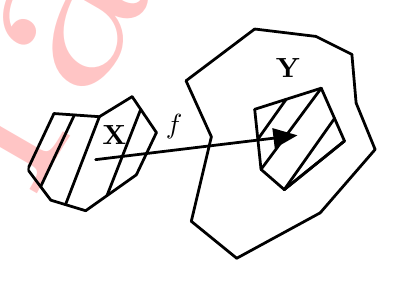
\begin{tikzpicture}[line cap=round,line join=round,>=triangle 45,x=1.2cm,y=1.2cm]
\clip(-2,-1.0) rectangle (1.8,1.5);
\draw [line width=1pt] (-1.721731253191196,0.5912980126724741)-- (-2,0);
\draw [line width=1pt] (-2,0)-- (-1.7552735699411093,-0.32552531182516203);
\draw [line width=1pt] (-1.7552735699411093,-0.32552531182516203)-- (-1.3863080856920604,-0.43733303432487375);
\draw [line width=1pt] (-1.3863080856920604,-0.43733303432487375)-- (-0.8496310176934437,-0.05718677782585391);
\draw [line width=1pt] (-0.8496310176934437,-0.05718677782585391)-- (-0.6371963449439912,0.390044112172993);
\draw [line width=1pt] (-0.6371963449439912,0.390044112172993)-- (-0.8943541066933284,0.7701903686720128);
\draw [line width=1pt] (-0.8943541066933284,0.7701903686720128)-- (-1.240958046442435,0.5577556959225606);
\draw [line width=1pt] (-1.240958046442435,0.5577556959225606)-- (-1.721731253191196,0.5912980126724741);
\draw [line width=1pt] (-0.3241347219447982,0.9379019524215805)-- (-0.05579618794548982,0.3453210231731083);
\draw [line width=1pt] (-0.05579618794548982,0.3453210231731083)-- (-0.2682308606949423,-0.5491407568245855);
\draw [line width=1pt] (-0.2682308606949423,-0.5491407568245855)-- (0.21254234605381853,-0.9404677855735766);
\draw [line width=1pt] (0.21254234605381853,-0.9404677855735766)-- (1.0958233538015418,-0.4596945788248161);
\draw [line width=1pt] (1.0958233538015418,-0.4596945788248161)-- (1.6772235108000433,0.21115175617345425);
\draw [line width=1pt] (1.6772235108000433,0.21115175617345425)-- (1.475969610300562,0.7031057351721858);
\draw [line width=1pt] (1.475969610300562,0.7031057351721858)-- (1.4312465213006773,1.2174212586708597);
\draw [line width=1pt] (1.4312465213006773,1.2174212586708597)-- (1.0511002648016572,1.4074943869203698);
\draw [line width=1pt] (1.0511002648016572,1.4074943869203698)-- (0.4026154743033286,1.485759792670168);
\draw [line width=1pt] (0.4026154743033286,1.485759792670168)-- (-0.3241347219447982,0.9379019524215805);
\draw [line width=1pt] (0.4026154743033286,0.6360211016723588)-- (0.4697001078031557,0);
\draw [line width=1pt] (0.4697001078031557,0)-- (0.7156770973025217,-0.21371758932545032);
\draw [line width=1pt] (0.7156770973025217,-0.21371758932545032)-- (1.352981115550879,0.3005979341732236);
\draw [line width=1pt] (1.352981115550879,0.3005979341732236)-- (1.107004126051513,0.8596365466717822);
\draw [line width=1pt] (1.107004126051513,0.8596365466717822)-- (0.4026154743033286,0.6360211016723588);
\draw [line width=1pt] (1.107004126051513,0.8596365466717822)-- (0.4697001078031557,0);
\draw [line width=1pt] (1.352981115550879,0.3005979341732236)-- (0.7156770973025217,-0.21371758932545032);
\draw [line width=1pt] (0.4360105988993155,0.31940606141757377)-- (0.7358659533977432,0.7418149045594744);
\draw [line width=1pt] (1.2477979256711231,0.5396506384453954)-- (0.7156770973025217,-0.21371758932545032);
\draw [line width=1pt] (-1.5055106601556578,0.576212855018832)-- (-1.8625329718453103,-0.1828531442025503);
\draw [line width=1pt] (-1.240958046442435,0.5577556959225606)-- (-1.5994753090588438,-0.3727369060319093);
\draw [line width=1pt] (-0.8036157369761233,0.6360553873509273)-- (-1.1607208986378066,-0.2775421101614441);
\draw [->,line width=1pt] (-1.280815773013133,0.10338031512207481) -- (0.8546440287963795,0.36066462859310017);
\draw (-1.3118161449035616,0.5639825130570472) node[anchor=north west] {$\mathbf{X}$};
\draw (0.5229817124863821,1.2729868547729377) node[anchor=north west] {$\mathbf{Y}$};
\draw (-0.64190301641527104,0.68352811967084686) node[anchor=north west] {$f$};
\end{tikzpicture}
\caption{映射$f$将$X$对应到$Y$中的子集,$Y$中的阴影是$f$的值域$f(X)$。}
\end{wrapfigure}

如图1.6所示,我们将输出的$f(x)$称作输入的$x$在映射$f$之下的\textbf{像(image)}\index{像(image)}。因此,根据之前映射的定义,$x\in X$ 有且只有一个像。如果映射$f:X\xrightarrow{}Y$和映射$g:X\xrightarrow{}Y$的\textbf{像}是一样的,$f(x)=g(x),\forall x \in X$,那么这两个映射是\textbf{相等的}。所有像所构成的集合我们称作$f$的\textbf{值域(range)}\index{值域(range)},记作$f(X)$。此外,我们将集合$X$称作\textbf{定义域(Domain)}\index{定义域(Domain)},将集合$Y$称为\textbf{陪域(Co-domain)}\index{陪域(Co-domain)}或者\textbf{目标域(target space)}\index{目标域(target space)}。

关于函数和映射我们还需要明确定义中的概念。\textbf{1. }定义域中\textbf{所有的元素}都必须要映射到陪域上的某个元素。\textbf{2.}定义域中的任意一个元素必须要\textbf{唯一}的映射到陪域上。也就是说任意一个$x$\textbf{必须有对应并且只能对应一个}$f(x)$,不过一个$f(x)$\textbf{不必须要有对应且可以对应多个}$x$。

\begin{defn}
映射$f: A \xrightarrow{} B$的$\Gamma_f$\textbf{图像(Graph)}\index{图像(Graph)}是$A \times B$的子集,定义为$\Gamma_f=\{(a,f(a))|a\in A\}\subset A \times B$。
\end{defn}

定义1.2.4确实有些让人迷惑,不过我们思考后应该就能够很快的发现它不过就是定义了我们初中就学过的函数图像。我们先从最为熟悉的实数函数来考虑,然后很容易地就可以注意到$(a,f(a))$说的不过就是函数线条上的任意一个点,那么这些点所构成的集合$\Gamma_f$自然就是函数图像了。那么,我们为什么要强调他是$A\times B$的子集呢?对于实数函数来说,$A\times B$无非就是整个笛卡尔坐标系的$xy$平面。我们的函数图像要在$xy$平面上或者范围里自然也是必须且重要的。

\begin{exmp}
集合$C$存放了三个不同的硬币$\{a,b,c\}$,假设一个函数$f$会将其对应到有正反两种状态构成的集合$S=\{0,1\}$上,那么就会有$2^3 = 8$种可能的映射和其图像。它们分别是:\\
$\Gamma_f1 = \{(a,0),(b,0),(c,0)\}, \Gamma_f2 = \{(a,1),(b,0),(c,0)\},\\
\Gamma_f3 = \{(a,0),(b,1),(c,0)\},\Gamma_f4 = \{(a,0),(b,0),(c,1)\}, \\
\Gamma_f5 = \{(a,1),(b,1),(c,0)\},\Gamma_f6 = \{(a,1),(b,0),(c,1)\},\\
\Gamma_f7 = \{(a,0),(b,1),(c,1)\}, \Gamma_f8 = \{(a,1),(b,1),(c,1)\}$\\
将大小为$N$的集合映射到大小为$n$的集合上会带来$n^N$种映射。
\end{exmp}

\subsection{序列(Sequence)}
\textbf{接下来的内容是一个十分重要的综合性例子,我们将会探讨如何运用集合和映射的思想,有艺术性地创造和定义一个新的结构。}
\begin{defn}
如果$\mathbb{Z}^{+a}_0 = \{0,1,2,\cdots,a\}$并且$Y$是任意集合,那么任何\textbf{映射}$l:\mathbb{Z}^{+a}_0 \xrightarrow{} Y$都叫做$Y$上的\textbf{序列}。我们将序列\textbf{定义域}中的任意一个元素$n\in\mathbb{Z}^{+a}_0 $叫做\textbf{索引},序列$l$的一个\textbf{像},$l(n)=u_n \in Y$称作序列的\textbf{项},这样序列$l$就记作$[u_n]$。
\end{defn}

既然提到了序列,这里我们不妨就来给它个定义。\textbf{序列(Sequence)}\index{序列(Sequence)}通俗的讲就是将一堆事物按照顺序且可以重复的放在一起。用数学的话来说,\textbf{一堆事物}就指的是\textbf{集合},把一堆事物按照规则放在一起指的就是\textbf{映射},\textbf{序列}就是把一个集合\textbf{有规则映射到}另一个集合上从而体现\textbf{顺序和可重复性}。\begin{wrapfigure}{r}{4cm}
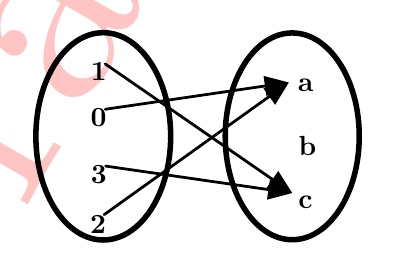
\begin{tikzpicture}[line cap=round,line join=round,>=triangle 45,x=1.2cm,y=1.2cm]
\clip(-1.8,-1.12) rectangle (1.8,1.15);
\draw [rotate around={90:(-1,0)},line width=2pt] (-1,0) ellipse (1.316387979510347cm and 0.8560825384268349cm);
\draw [rotate around={90:(1,0)},line width=2pt] (1,0) ellipse (1.3130581708736389cm and 0.8509534417922207cm);
\draw (-1.2344629386286757,0.8879887443175114) node[anchor=north west] {$\mathbf{1}$};
\draw (-1.2384221308940924,0.4010080956712348) node[anchor=north west] {$\mathbf{0}$};
\draw (-1.2344629386286757,-0.20870751320296518) node[anchor=north west] {$\mathbf{3}$};
\draw (-1.2423813231595094,-0.7313208922379938) node[anchor=north west] {$\mathbf{2}$};
\draw (0.9570107708760184,0.7058659001083348) node[anchor=north west] {$\mathbf{a}$};
\draw (0.9649291554068521,0.10406867576496857) node[anchor=north west] {$\mathbf{b}$};
\draw [->,line width=1pt] (-0.9791145611060509,0.7661506259137978) -- (1,-0.6);
\draw [->,line width=1pt] (-0.9791145611060509,0.2861885453743965) -- (0.9634091349353068,0.569630718921287);
\draw [->,line width=1pt] (-0.9904522480479265,-0.8286840039100397) -- (0.9634091349353069,0.5696307189212871);
\draw [->,line width=1pt] (-0.9753353321254257,-0.3147088625450115) -- (1,-0.6);
\draw (0.9609699631414352,-0.5333612789671496) node[anchor=north west] {$\mathbf{c}$};
\end{tikzpicture}
\caption{序列$[a,c,a,c]$}
\end{wrapfigure}
虽然说集合中的元素有无序性,但是集合本身可以是建立在一个有序的框架条件上的,有限大小为$a$的\textbf{非负整数集}$\mathbb{Z}^{+a}_0 = \{0,1,2,\cdots,a\}$就是一个天然就有顺序的集合。我们的直觉可能会是要把一个集合当作输入映射到正整数集上\textbf{排号}输出。然而这是\textbf{错误}的,只要稍加思考我们就会发现如果要满足\textbf{待排序集合}上的事物具有\textbf{可重复性},那么根据映射性质它就不能作为定义域输入,因为定义域上的元素只能有一个对应。因此,\textbf{正确}的做法是将正整数集作为定义域映射到一个集合上,由此达到为该集合排序的目的。具体的映射作为序列的例子如图1.7所示,序列$f:\mathbb{Z}^{+a}_0 \xrightarrow{} {a,b,c}$将$0$对应到$a$以此类推,排列在一起构成序列$[a,c,a,c]$。

\begin{thm}
如果有映射$f:X \xrightarrow{}Y$和映射$g: Y\xrightarrow{}Z$,那么$f$与$g$的\textbf{复合(composition)}\index{复合(composition)} $h:X \xrightarrow{} Z$也是一个映射,记作$h= g\circ f$。此外,复合映射$h$的像为$h(x)=g(f(x))$。
\end{thm}
\begin{exmp}
映射$f:\{1,2\} \xrightarrow{} \{3,4\}$和$g: \{3,4\}\xrightarrow{}\{5,6\}$的复合函数为$h:\{1,2\} \xrightarrow{} \{5,6\}$。如果$\Gamma_f=\{(1,3),(2,4)\},\Gamma_g=\{(3,5),(4,6)\}$,那么$\Gamma_h=\{(1, 5), (2, 6)\}$。
\end{exmp}
\begin{defn}
如果有映射$f:X \xrightarrow{} Y$并且$A$是集合$X$的子集,那么$f(A)=\{f(x)|x \in A\}$就是$A$的\textbf{像}。反过来,如果$B \subseteq Y$,那么$f^{-1}(B) = \{x \in X | f(x) \in B\}$就是$B$的\textbf{原像(Preimage)}\index{原像(Preimage)}。如果$B$由单个元素$b$组成的,则$f^{−1}(B)=\{x\in X | f(x)= b\}$是由$X$中的所有映射到$B$的元素组成的一个\textbf{纤维(Fiber)}\index{纤维(Fiber)}。
\end{defn}

由于定义域中的多个元素可以映射到一个陪域中的元素上,同时不一定所有陪域上的元素都要有对应。因此,一个纤维不一定是单元素集合而是可以由\textbf{零个及以上}的元素构成的集合。根据定义,定义域子集可以\textbf{映射}到一个陪域子集\textbf{(像)}上,然而如果推广一下我们之前所讨论的内容,就会发现陪域子集对应到定义域子集\textbf{(原像)}上的联系\textbf{不一定}是满足映射条件的。因而若是想要了解在怎样的条件下陪域也可以\textbf{映射}到定义域上的话,我们就需要先来明确定义和讨论映射的方式和规则。

\begin{defn}
如果$x_1,x_2 \in X$并且每当$f(x_1)=f(x_2)$都有$x_1 = x_2$,那么就意味着任意$f(x)\in Y$最多只有一个原像$f^{-1}(f(x)) \in X$,我们将这样的映射$f$称作\textbf{单射(injective or one-to-one)}\index{单射(injective or one-to-one)},记作$1-1$。如果映射$f$满足$f(X)=Y$,那么$f(x)\in Y$至少有一个原像$f^{-1}(f(x)) \in X$,我们将这样的映射$f$称作\textbf{满射(onto or surjective)}\index{满射(onto or surjective)}。如果$f$既是单射又是满射,那么任意的像$f(x)\in Y$一定\textbf{有且只有一个}原像,我们称其为\textbf{双射(bijective)}\index{双射(bijective)}。
\end{defn}

在我看来数学上的定义大致分为\textbf{规则性}定义和\textbf{结构性}定义。一般来说,我都会在能力范围内尽可能的长篇大论地深入探讨\textbf{结构性}定义,就像之前探讨该如何定义序列那样,因为其中往往可能会有着很多\textbf{深刻}的思想和图景。对于\textbf{规则性}定义来说,定义本身并不会对我们的理解起到很大的帮助,更多的时候我们对其的理解是建立在对具体例子思考和\textbf{归纳}后得出的。
\subsection{基数(Cardinality)}
当你尝试思考了不同实例后,或者说你天赋异禀一开始就从定义显然的知道了下面的规律。单射的定义域元素数量一定\textbf{小于等于}陪域,满射的定义域元素数量一定\textbf{大于等于}陪域,双射的定义域元素数量\textbf{一定等于}陪域。如果定义域和陪域元素数量\textbf{相等},那么无论是\textbf{单射}还是\textbf{满射}其效果彼此相同且都和\textbf{双射一样}。看来集合的\textbf{元素数量}还是个挺重要的玩意儿,我们不妨给它起个名字-\textbf{基数(cardinal)}\index{基数(cardinal)}。集合$\mathbb{N}_n = \{1,2,\cdots,n\}$是\textbf{有限的(finite)}\index{有限的(finite)}并且基数为$n$,任意集合$A$是有限的如果$A$和$\mathbb{N}$是等价的$A \bowtie \mathbb{N}_n$。也就是集合$A$和$\mathbb{N}$之间存在\textbf{双射},这里集合$A$的基数也是$n$。如果$A$不是有限的,那么它就是\textbf{无限的(infinite)}\index{无限的(infinite)}。一个集合(所有自然数的集合)可以与其子集(例如所有偶数的集合)双射,这是任意无限集共有的特性。如果$A\bowtie \mathbb{N}$,那么$A$是\textbf{可数的(countably infinite)}\index{可数的(countably infinite)}。如果集合$A$既不是有限的,也不是可数的,那么它是\textbf{不可数的(uncountable)}\index{不可数的(uncountable)}。

在\textbf{闭区间}$[0,1]$中间挖去一个\textbf{开区间}$(\frac{1}{3},\frac{2}{3})$,也就像是把一根线段平均分成三份,拿走中间的一份,剩下了的就是$[0,\frac{1}{3}]\cup[\frac{2}{3},1]$,继续这样的操作有$[0,\frac{1}{9}]\cap[\frac{2}{9},\frac{1}{9}]\cap[\frac{2}{3},\frac{7}{9}]\cap[\frac{8}{9},1]$,让其无限地一直挖下去,剩下来的部分就是\textbf{康托尔集(Cantor set)}\index{康托尔集(Cantor set)},康托尔集的基数和原先的$[0,1]$是一样的。
\subsection{可逆映射,商映射}
\begin{thm}
结合之前我们讨论过的\textbf{复合函数},如果$f\circ g$是单射,则$g$\textbf{一定}是单射而$f$\textbf{不必}是单射。如果$f\circ g$为满射,则$g$\textbf{不必}是满射而$f$\textbf{一定}是满射。如果$f\circ g$是双射,则$g$\textbf{不必}是满射而$f$\textbf{不必}是单射。
\end{thm}

回到我们之前所讨论的原像上,如果是映射是\textbf{单射}的话,那么\textbf{陪域}上可能存在没有与\textbf{定义域}对应的元素,因而像对应到原像\textbf{不满足}映射的条件。如果是\textbf{满射},那么尽管\textbf{陪域}上所有元素都能够有对应,然而其不一定是\textbf{唯一}的对应,因此还是\textbf{不满足}映射性质。如果映射$f$为\textbf{双射},那么其\textbf{陪域和定义域}的元素数量根据定义是\textbf{相等}的并且对于任意一个$y\in Y$都有且只有一个$x\in X$使得$f(x)=y$。这样一来就满足了映射的性质,我们就有$f^{-1}:Y \xrightarrow{} X$满足$f^{-1}(y)=x$。
\begin{defn}
映射$f$是\textbf{可逆的(invertible)}\index{可逆的(invertible)}并且$f^{-1}$是$f$的\textbf{反函数(inverse function)}\index{反函数(inverse function)},如果$f(x)=y \iff f^{-1}(y)=x,\forall y\in Y,x \in X$。或者说,$f$可逆当且仅当有$f^{-1}(f(x))=x $并且$ f(f^{-1}(y)) = y, \forall y\in Y,x \in X$也就是$f^{-1}\circ f = id_Y \land f\circ f^{-1} = id_X$。
\end{defn}
\begin{exmp}
$f(x)=y=e^x$是可逆的其反函数为$f^{-1}(y) = x =\ln y $,因为$f^{-1}(f(x))=\ln (e^x)=x $并且$ f(f^{-1}(y)) = e^{\ln y}= y$。
\end{exmp}
\begin{exmp}
$f(x)=y=2x+3$是可逆的其反函数为$f^{-1}(y)=x = \frac{y-3}{2}$或者$f^{-1}(x)= \frac{x-3}{2}$。设映射$f:X \xrightarrow{}Y$图像的子集为:$\{(3, 0), (5, 1), (9, 3), (7, 2)\}$,那么其逆映射$f^{-1}:Y \xrightarrow{}X$对应的图像子集为$\{(2, 7), (1, 5), (0, 3), (3, 9)\}$。
\end{exmp}

我们不难发现映射图像和逆映射图像集合$\Gamma_f$和$\Gamma_{f^{-1}}$上的每个有序对是有\textbf{一对一关系}(双射)的且有\textbf{对称性},设$a\vartriangleright b \equiv (a,b)$,那么就有$(x,y)\implies(y,x)$。有序对的对称只是一个比较直观的展示,真正的对称是发生在映射本身上的$f:X \xrightarrow{}Y\implies f^{-1}:Y \xrightarrow{}X$。那么,我们可以定义一个求逆的映射$p:\Gamma_f \xrightarrow{}\Gamma_{f^{-1}}$。我们规定的求逆映射正是利用了映射与逆映射图像之间的对称性,从而交换有序对中$x,y$的位置得出的。在有序对内位置被对调的时候,满足条件$x=y$的有序对是\textbf{前后不会发生改变}的也就是图像集合$\{(x,y)|x=y,x\in X ,y\in Y\}$。因而$f(x)$和$f^{-1}(x)$是关于$f(x)=x$镜像对称的。
\begin{exmp}
利用对称性\textbf{展示}复合函数$(g\circ f)^{-1} = f^{-1} \circ g^{-1}$:\\
复合映射$g\circ f = X\xrightarrow{f}Y\xrightarrow{g}Z$ 的\textbf{逆}为 $f^{-1} \circ g^{-1}= Z\xrightarrow{g^{-1}}Y\xrightarrow{f^{-1}}X$。
\end{exmp}
\begin{thm}
给定映射$f:X \xrightarrow{} Y$,集合$X$上有\textbf{等价关系}$x_1 \bowtie x_2 \implies f(x_1)=f(x_2)$。\textbf{等价类}是$X$的子集,其所有元素映射到$Y$中的同一元素。若是$X,Y$有\textbf{相同基数}且$f$为单射或者满射,则有\textbf{等价关系}$X \bowtie Y$。
\end{thm}

\textbf{证明}可考虑等价关系性质:自反,对称,传递。关于$x_1 \bowtie x_2$的\textbf{等价类}也就是说,一个\textbf{满射的陪域}中任意元素的\textbf{原像}都可以被认为是一个等价类$[x]=f^{-1}(f(x))$,因而我们可以得到以该\textbf{等价类}组成的原定义域的\textbf{商集}。
\begin{defn}
等价类是$X$的子集,其所有元素映射到$Y$中的同一个点。也就是说,有个与之对应的映射$\tilde{f}:X/\bowtie \, \xrightarrow{} Y$,或者$\tilde{f}([x])=f(x)$,我们将其称之为\textbf{商映射(Quotient Map or Factor Map)}\index{商映射(Quotient Map)}。
\end{defn}

比如,设函数为$f(x)=x^2$就有$\tilde{f}(\{\pm \sqrt{x}|x\in X\})=f(x)$。
\begin{thm}
映射$\tilde{f}:X/\bowtie \, \xrightarrow{} f(X)$是\textbf{双射}。
\end{thm}

\textbf{证明:}\textbf{商映射是单射},因为$\tilde{f}([x_1])=\tilde{f}([x_2])\implies f(x_1) = f(x_2)$,所以$x_1$和$x_2$属于同一等价类$[x_1]=[x_2]$。映射$f$为\textbf{满射}当且仅当$f(X)=Y$,并且$f$满射意味着每一个$y\in Y$都有与之对应的\textbf{等价类}。如果$f$\textbf{不是满射},则\textbf{任意的}$y\in f(X)$都有对应的\textbf{等价类}使得$\tilde{f}$既是\textbf{满射}也是\textbf{单射}。$\clubsuit$

接下来我们将会讨论几个较为复杂的综合性例子作为映射部分的总结和巩固。第一个例子需要我们对\textbf{区间(Intervals)}\index{区间(Intervals)}有最为基本的认识。
\begin{defn}
设$a,b \in R$,\textbf{开(Open)区间:}$]a,b[=\{x\in \mathbb{R}|a<x<b\}$。\textbf{闭(Close)区间:}$[a,b]=\{x\in \mathbb{R}|a \leq x \leq b\}$。另外,$[a,b[=\{x\in \mathbb{R}|a \leq x < b\},]a,b]=\{x\in \mathbb{R}|a < x \leq b\}$。
\end{defn}
\begin{wrapfigure}{r}{4cm}
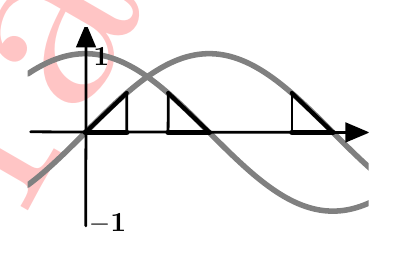
\begin{tikzpicture}[line cap=round,line join=round,>=triangle 45,x=1cm,y=1cm]
\clip(-0.7344476611331308,-1.25) rectangle (3.59467498749326,1.33);
\draw[line width=2pt,color=gray,smooth,samples=100,domain=-0.7344476611331308:5.509467498749326] plot(\x,{sin(((\x))*180/pi)});
\draw[line width=2pt,color=gray,smooth,samples=100,domain=-0.7344476611331308:5.509467498749326] plot(\x,{cos(((\x))*180/pi)});
\draw [line width=2pt] (0,0)-- (0.5233747712729805,0);
\draw [line width=1pt] (0.5233747712729805,0)-- (0.5248721669066926,0.5011023835426925);
\draw [line width=1.5pt] (0,0)-- (0.5233747712729805,0.5011023835426925);
\draw [line width=1pt] (2.62218782115019,0.4963635520466573)-- (2.62218782115019,0);
\draw [line width=2pt] (3.141592653589777,0)-- (2.62218782115019,0);
\draw [line width=1.5pt] (1.05,0.5)-- (1.5733747712729805,0);
\draw [line width=1pt] (1.0504580343396472,0.497173686087218)-- (1.048960638705935,0);
\draw [line width=2pt] (1.048960638705935,0)-- (1.5707963281932422,0);
\draw [line width=1.5pt] (2.62,0.5)-- (3.14,0);
\draw (-0.025282362295306036,1.2033788145557728) node[anchor=north west] {$\mathbf{1}$};
\draw (-0.08234163921329193,-0.9059228654847326) node[anchor=north west] {$\mathbf{-1}$};
\draw [->,line width=1pt] (0.003247276163686912,-1.1871435874376635) -- (0.007322938800685904,1.3845995365087036);
\draw [->,line width=1pt] (-0.6977666974001397,0.007025565203042694) -- (3.606133047270796,-0.0011257600709552998);
\end{tikzpicture}
\caption{三角函数}
\end{wrapfigure}

映射$\rm sin: \mathbb{R} \xrightarrow{} [-1,1] \subset \mathbb{R}$ 和 $\rm cos: \mathbb{R} \xrightarrow{} [-1,1] \subset   \mathbb{R}$ 有关于陪域元素$0$的原像为:$\rm sin^{-1}(0)=\{n\pi\}^{\infty}_{n=-\infty}, \rm cos^{-1}(0)=\{\frac{\pi}{2}+ n\pi\}^{\infty}_{n=-\infty}.$
类似的,\textbf{闭区间}$[0,\frac{1}{2}]\subset \mathbb{R}$的原像,包含所有$x$轴上的粗线的\textbf{并集}。如图1.8所示,$x$轴上的所展示的粗线为函数$\rm sin$或$\rm cos$的\textbf{原像}$\rm sin^{-1}[0,\frac{1}{2}]$或者$\rm cos^{-1}[0,\frac{1}{2}]$的子集。函数图像上的粗线为$\rm sin$或者$\rm cos$的\textbf{像}。

\begin{defn}
一个从$X$到$Y$的\textbf{$n$元映射(n-ary map)}\index{$n$元映射(n-ary map)}为映射$f:X^n \xrightarrow{} Y$有$f(x_1,\cdots ,x_n) = y$,这就是我们所熟悉的多元函数。
\end{defn}
\textbf{射影映射(projection map)}\index{射影映射(projection map)}为$\rm Proj_i$ $= X^n \xrightarrow{} X_i$给定 $\mathbf{x}=(x_1,\cdots,x_n)\in X^n,\rm Proj_i$ $(\mathbf{x})=x_i$。
\begin{defn}
给定任意集合$X$上有等价关系$\bowtie$,那么根据定义自然\textbf{(natural or canonical  map)}就有一个称作\textbf{正则射影(canonical projection)}\index{正则射影(canonical projection)}的映射$p:X \xrightarrow{} X/\bowtie$,将一个集合$X$映射到该集合所以等价类组成的商集$X/\bowtie$上。对于任意的$x\in X$也就是$p(x)=[x]$。
\end{defn}

因为不同的$x$可以映射到同一等价类上$p(x_1)=p(x_2)\implies x_1 \bowtie x_2$,所以\textbf{射影}显然是满射非单射的。如果该等价关系为恒等映射$\bowtie\, =\rm id_X$,那么该映射就变为双射,记作$X \cong X/\rm id_X$。

\begin{exmp}
\textbf{单射和满射依赖于定义域和值域。}映射$f:\mathbb{R} \xrightarrow{} \mathbb{R},f(x)=x^3$和$g:\mathbb{R} \xrightarrow{} ]-1,1[,g(x)=\tanh x$都是\textbf{双射}。接下来,我们就映射$f(x)=x^2$来考虑在不同定义域和值域下的情况。\\
\textbf{1.满射非单射} $f:\mathbb{R} \xrightarrow{} \mathbb{R}^+$,$\pm x$都二对一映射到全体正实数上。\\
\textbf{2.单射非满射} $f:\mathbb{R}^+ \xrightarrow{} \mathbb{R}$,$+ x$一对一映射到实数的正数部分$x^2$上。\\
\textbf{3.双射} $f:\mathbb{R}^+ \xrightarrow{} \mathbb{R}^+$,$+ x$都一对一映射到全体正实数上。\\
\textbf{4.非单射非满射} $f:\mathbb{R} \xrightarrow{} \mathbb{R}$,$\pm x$二对一映射到实数的正数部分$x^2$上。
\end{exmp}
\begin{exmp}
设$M^{n×n}$表示$n×n$实矩阵的集合。定义一个求\textbf{行列式(determinant)}\index{行列式(determinant)}的函数$det:
M^{n×n}\xrightarrow{} \mathbb{R}$。这个映射是满射而不是单射,因为不同矩阵可以有同一个行列式且行列式的取值范围为整个实数集。
\end{exmp}
\begin{exmp}
映射$f:\mathbb{C} \xrightarrow{} \mathbb{R},f(z)=|z|$ 既不是单射也不是满射。原像$f^{-1}(1)$为复平面上的\textbf{单位圆(unit circle)}\index{单位圆(unit circle)}。
\end{exmp}

不同复数的模长可以相同因此不单射。复数的模一定是零和正实数的并集$f(\mathbb{C})=\{0\}\cup  \mathbb{R}^+$故不满射。该映射可以引申出一个$\mathbb{C}$上的\textbf{等价关系}:如果$z_1,z_2$的模长相等在同一个圆上,那么就有$z_1 \bowtie z_2$。这样我们就有商集$\mathbb{C}/\bowtie$为复平面上圆心为原点的所有圆的集合。$\tilde{f}:\mathbb{C}/\bowtie \xrightarrow{} \{0\}\cup  \mathbb{R}^+$是将每个圆对应到其半径的一个双射。正如我们之前在\textbf{$n$元映射}的定义中所见,映射的定义域可以是集合的笛卡尔积。和二元关系一样$n$元映射中的\textbf{二元映射}$f: X \times X \xrightarrow{} Y$也是尤为的重要的。
\begin{exmp}
\textbf{点乘}就是将任意两个向量对应到实数集的二元映射$f: \mathbb{R}^n \times \mathbb{R}^n \xrightarrow{} \mathbb{R}$,设向量$\mathbf{a,b}=(a_1,\cdots,a_n),(b_1,\cdots,b_n)$,给定$f(\mathbf{a,b})=\mathbf{a\cdot b}$。
\end{exmp}
\begin{defn}
对于\textbf{二元映射}$f: X \times X \xrightarrow{} Y$,如果有$Y=X$,我们称这样的映射为\textbf{二元运算(binary operation)}\index{二元运算(binary operation)}。从集合$X$中任意选取两个元素映射到一个仍然属于$X$的元素上的运算是\textbf{封闭的(closed)}\index{封闭的(closed)}。
\end{defn}
\begin{exmp}
实数上的四则运算的加、减、乘、除都是二元运算。\textbf{叉乘}就是将任意两个向量对应到新向量的二元运算$f: \mathbb{R}^n \times \mathbb{R}^n \xrightarrow{} \mathbb{R}^n$,设向量$\mathbf{a,b}=(a_1,\cdots,a_n),(b_1,\cdots,b_n)$,给定$f(\mathbf{a,b})=\mathbf{a\times b}$。
\end{exmp}

\section{度量空间(Metric Space)}
尽管集合论是现代数学的根基,但它本身还是过于的抽象和形式化。因此,我们将会基于集合介绍更多的数学结构让它变得更为实用。数学上通常会以两种方式来实现这样的构造,对应于两类数学的主要分支—\textbf{代数(algebra)}\index{代数(algebra)}和\textbf{分析(analysis)}\index{分析(analysis)}。我们可以通过在一个集合上引入二元运算把它变成一个\textbf{代数结构}。例如,\textbf{向量加法}是封闭的二元运算。一个\textbf{群(group)}\index{群(group)}是由一种集合以及一个二元运算所组成的代数结构。使用集合的概念对分析学进行抽象时,还能引导出\textbf{开集}与\textbf{闭集}之类的\textbf{拓扑}性质,其中\textbf{连续性}的概念起着关键作用。我们不会很的深入这两个领域,但我们还是会按照循序直观地介绍一些我们所需要的最为基本的概念,那我们先从介绍\textbf{度量空间}开始。

\begin{defn}
集合$X$是一个\textbf{度量空间},若任意两点$x,y$经过\textbf{二元映射}$d:X\times X \xrightarrow{}\mathbb{R}$ 能够对应到$x,y$之间的距离$d(x,y)$上,且满足:\\
$\cdot \qquad$ \textbf{1.} $d(x,y) \geq 0 \, \forall x,y $ \textbf{非负性:} 两点间距离永不为负\\
$\cdot \qquad$ \textbf{2.} $d(x,y)=0 \iff x=y$ \textbf{唯一性:} 两点相等距离为零\\
$\cdot \qquad$ \textbf{3.} $d(x,y)=d(y,x)$ \textbf{对称性:} 两点互换距离不变\\
$\cdot \qquad$ \textbf{4.} $d(x,y)\leq d(x,z)+d(z,y)$ \textbf{三角不等式} 
\end{defn}

看到这样的定义很多人或许都会先入为主的带入笛卡尔坐标系或者欧几里得几何上的点。这或许是抽象的程度和深度不足的体现,因此我们在阅读定义时,更多的是要思考和分析那些从对象中\textbf{抽象}出来的\textbf{性质}。我们需要将目光暂时从对象上移开,也就是说,我们需要时刻的清楚\textbf{集合$X$不需要任何的结构,任意随便的什么集合都可以是集合$X$。} 因此,度量空间的关键是距离函数对于任意两个元素满足的那四个性质。
\begin{thm}
如果在距离函数$d$下,$X$是一个度量空间,那么任意一个$X$的非空子集$S$也是函数$d$下的一个度量空间。
\end{thm}

很显然,因为任意$X$中的两个元素在距离函数$d$下都满足四个性质的话,那么其部分元素构成的子集一样满足。
\begin{exmp}\textbf{各种度量空间的例子:}\end{exmp}

\textbf{1.}我们所最为熟知也是很重要的一个度量空间就是\textbf{欧氏空间(Euclidean space)}\index{欧氏空间(Euclidean space)}$\mathbb{R}^n$。设非负实数距离函数为二元映射$d: \mathbb{R}^n \times \mathbb{R}^n \xrightarrow{} \mathbb{R}^+ \cup \{0\}$,设向量$\mathbf{a,b}=(a_1,\cdots,a_n),(b_1,\cdots,b_n)$,$d(\mathbf{a,b})=\mathbf{||a - b||}=\sqrt{(a_1-b_1)^2,\cdots,(a_n-b_n)^2}$。此外,\textbf{复平面}也可以被看做一个二维的欧氏空间,尽管复数不能比较大小,复数之间是有距离的。因而我们可以将实数上的分析学思想搬到复数上。

\textbf{2.}\textbf{有理数集}为实数集的子集,那么易证明其广义笛卡儿积也满足$\mathbb{Q}^n \subset \mathbb{R}^n$,因此在\textbf{同一}距离函数下,$\mathbb{Q}^n$ 也是度量空间。

\textbf{3.} 设$X$为包含球面上所有点的集合。我们可以定义两个不同的距离函数。$d_1(P,Q)$为连接球面上点$P,Q$的\textbf{弦长(chord length)}\index{弦长(chord length)},$d_2(P,Q)$为穿过点$P,Q$最大的一个圆上以$P$为起点$Q$为终点的\textbf{弧长}。对于$d_2$如果三个点有两个是\textbf{极点}$N,S$,那么三角不等式就变为等式$d(N,S)=d(N,P)+d(P,N)$,因为极点的弦穿过球心,因而穿过极点的任意一个圆都为球面最大的圆,并且能够覆盖整个球面的所有点,使得三个点总会在同一弧上。

\textbf{4.} 让$C^0[a,b]$为闭区间$[a,b]$上的连续实值函数$[a,b] \xrightarrow{} \mathbb{R}$的集合,$f,g \in C^0(a,b)$。我们可以定义距离函数$d(f,g)=\int^b_a|f(x)-g(x)|dx$。这个距离描述的就是函数$f,g$的图像在区间$[a,b]$上所包围起来的面积。

\textbf{5.} 让$C_B(a,b)$为闭区间$[a,b]$上的\textbf{有界(bounded)}\index{有界(bounded)}连续实值函数$[a,b] \xrightarrow{} \mathbb{R}$的集合,$f,g \in C_B(a,b)$。距离函数$d(f,g)=\max\limits_{a\leq x\leq b}  \{|f(x)-g(x)|\}$。这个距离描述的就是函数$f,g$的图像在区间$[a,b]$上在同一$x$上最长的一条垂线距离。

\begin{wrapfigure}{r}{4cm}
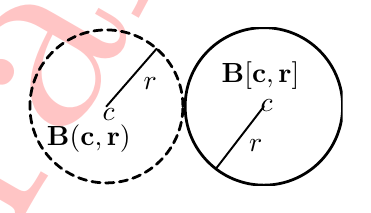
\begin{tikzpicture}[line cap=round,line join=round,>=triangle 45,x=1cm,y=1cm]
\clip(-2,-1) rectangle (2,1);
\draw [line width=1pt,dash pattern=on 3pt off 2pt] (-1,0) circle (0.9716740744441595cm);
\draw [line width=1pt] (1,0) circle (1cm);
\draw [line width=0.7pt] (-1,0)-- (-0.3621078649926808,0.732969392978123);
\draw [line width=0.7pt] (1,0)-- (0.3900285308210887,-0.7924233759725419);
\draw (-1.878815476177351,-0.1098249646026457) node[anchor=north west] {$\mathbf{B(c,r)}$};
\draw (0.3396248457651039,0.695560368687858) node[anchor=north west] {$\mathbf{B[c,r]}$};
\draw (-0.651764570312639,0.4887237279234368) node[anchor=north west] {$r$};
\draw (-1.172570149798875,0.0964473402667761) node[anchor=north west] {$c$};
\draw (0.6891074456774017,-0.3029613453472785) node[anchor=north west] {$r$};
\draw (0.8329285558027303,0.21071193618156376) node[anchor=north west] {$c$};
\end{tikzpicture}
\caption{开球,闭球}
\end{wrapfigure}

根据度量空间的定义,两点间距离为正实数也是欧几里得度量空间的性质。不过,相对论的\textbf{闵可夫斯基度量空间(Minkowskian metric space)}\index{闵可夫斯基度量空间}中距离的平方可以是负实数。由此看见,若要判定闵可夫斯基空间为度量空间的话,用\textbf{闵可夫斯基度量(Minkowski metric)}\index{闵可夫斯基度量}$s^2 = -t^2+x^2+y^2+z^2$是行不通的,也就是说\textbf{闵可夫斯基度量}不是该空间上的距离函数。

根据度量的性质,$B(c,0)=\emptyset;B[c,0]=\{c\}$。开球和闭球的定义会让我们不由自主的将其带入到欧氏空间,因此值得强调开球和闭球可以是在任意度量空间。如图1.9所示,我们也可以更为直观地将开球集合比作一个用虚线围成的圆盘,将闭球集合比作用实线围成的圆盘。
\begin{defn}
若$X$为度量空间有$c,x \in X, r \geq 0$,那么一个以$c$为球心$r$为半径的\textbf{开球(Open ball)}\index{开球(Open ball)}为$B(c,r)=\{x|d(c,x)<r\}$,也就是由所有到球心距离\textbf{小于}半径的点构成的集合。一个以$c$为球心$r$为半径的\textbf{闭球(Closed ball)}\index{闭球(Closed ball)}为$B[c,r]=\{x|d(c,x)\leq r\}$,也就是由所有到球心距离\textbf{小于等于}半径的点构成的集合。
\end{defn}

\begin{defn}
一个度量空间$X$上的\textbf{序列}是从自然数集到度量空间上的映射$\, x:\mathbb{N}\xrightarrow{}X$。该序列的像属于度量空间,$x(n)=x_n \in X$。我们用$\{x_n\}_{n=1}^\infty$来表示对序列所有项的枚举。
\end{defn}

我们在之前已经强调了序列的有序性。距离函数的规定使得在度量空间中点与点之间自然有了\textbf{“紧密度(closeness)”}的概念。因而,我们可以将序列引入到度量空间上去,为其增加元素间紧密度的新特性。

\begin{defn}
给定某个$x\in X$,若对于任意正实数$\epsilon > 0$,都存在自然数$N$,使得每当$n>N$时,都有一个围绕点$x$的开球$B(x_n,\epsilon)$,也就是$d(x_n,x)<\epsilon$,则序列$\{x_n\}_{n=1}^\infty$\textbf{收敛(converges)}\index{收敛(converges)}于$x$并记作$\lim_{n\xrightarrow{}\infty} d(x_n,x)=0$或者$x_n \xrightarrow{} x$。反之我们则称其为\textbf{发散(divergence)}\index{发散(divergence)}。\textbf{柯西序列(cauchy sequence)}\index{柯西序列(Cauchy sequence)}满足$\lim_{n,m\xrightarrow{}\infty} d(x_n,x_m)=0$
\end{defn}

\begin{wrapfigure}{r}{4cm}
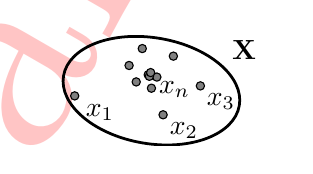
\begin{tikzpicture}[line cap=round,line join=round,>=triangle 45,x=1cm,y=1cm]
\clip(-1.5718299006210086,-0.6556772011272864) rectangle (1.6892234682789913,0.8434833978601843);
\draw [rotate around={-9.596109136014174:(-0.0002497100577637685,0.04317715463780169)},line width=1pt] (-0.0002497100577637685,0.04317715463780169) ellipse (1.1320442328054676cm and 0.6726719740565557cm);
\draw (-0.9573787921651138,-0.008995578294129537) node[anchor=north west] {$x_1$};
\draw (0.9,0.8) node[anchor=north west] {$\mathbf{X}$};
\draw (0.11018710018004402,-0.232120282482024) node[anchor=north west] {$x_2$};
\draw (0.5804653228529914,0.13517730748881765) node[anchor=north west] {$x_3$};
\draw (-0.027120410089429652,0.2793501932717648) node[anchor=north west] {$x_n$};
\begin{scriptsize}
\draw [fill=gray] (-0.9745422309487984,-0.02272632932107708) circle (1.5pt);
\draw[color=gray] (-0.9436480411381665,0.05107645744876512);
\draw [fill=gray] (0.1479466655041489,-0.26301447229265573) circle (1.5pt);
\draw[color=gray] (0.17884085531478086,-0.1892116855228135);
\draw [fill=gray] (0.2783888002601489,0.48187877091923803) circle (1.5pt);
\draw[color=gray] (0.30928299007078086,0.5556815576890802);
\draw [fill=gray] (-0.11637029176458794,0.5779940281078695) circle (1.5pt);
\draw[color=gray] (-0.08547610195395597,0.6517968148777117);
\draw [fill=gray] (-0.19349644671096647,0.15470004065068002) circle (1.5pt);
\draw[color=gray] (-0.1609952326021665,0.22957622079908066);
\draw [fill=gray] (0,0.07475827176667772) circle (1.5pt);
\draw[color=gray] (0.03123528177509666,0.14719171463739658);
\draw [fill=gray] (0.06878483222164179,0.21603632084368535) circle (1.5pt);
\draw[color=gray] (0.0998890369098335,0.29136460042034373);
\draw [fill=gray] (-0.04105846823902641,0.24605405204124142) circle (1.5pt);
\draw[color=gray] (-0.009956971305745441,0.3188261024742384);
\draw [fill=gray] (-0.026081660953634,0.22573857582752038) circle (1.5pt);
\draw[color=gray] (0.003773779721201926,0.2982299759338174);
\draw [fill=gray] (-0.009911235980575629,0.2731718224151583) circle (1.5pt);
\draw[color=gray] (0.020937218504886133,0.3462876045281331);
\draw [fill=gray] (-0.28386540284070827,0.36324378556546866) circle (1.5pt);
\draw[color=gray] (-0.2536778020340612,0.4355374862032909);
\draw [fill=gray] (0.6216575759338331,0.1042831176781859) circle (1.5pt);
\draw[color=gray] (0.652551765744465,0.1780859044480281);
\end{scriptsize}
\end{tikzpicture}
\caption{柯西序列}
\end{wrapfigure}
早在古希腊芝诺的乌龟就已经对趋近作为不断追赶动态过程这一思想有了大致的雏形,在数学上我们为了追求严格和精准的描述,巧妙地运用了不断选取$n>N$让$\epsilon$趋近于无穷小。

我们有时可能无法直接用该定义检验序列的敛散性,因为这需要给定我们一个$x$作为\textbf{极限点(Limit point)}\index{极限点(Limit point)}也是\textbf{聚集点(cluster point)}\index{聚集点(cluster point)}。不过如图1.12所示,我们还是可以用接下来的方法考察序列中点与点间的距离不断\textbf{缩小},随着$n$的取值不断\textbf{增大}。

\begin{defn}
一个\textbf{完备度量空间(complete metric space)}\index{完备度量空间}是所有柯西序列收敛的度量空间。
\end{defn}

\textbf{注意:柯西序列不一定是收敛的。}$\spadesuit$例如,设度量空间为有理数集$\mathbb{Q}$有度量$d(x,y)=|x-y|$,考虑序列$\{x_n\}_{n=1}^\infty$有$x_n=\sum^{n}_{k=1} (-1)^{k+1}/k$,这是一个柯西序列有$|x_m-x_n|\xrightarrow{} 0$(证明留做习题)。然而,$\lim_{n \xrightarrow{}\infty} x_n = \ln 2$ 不是\textbf{有理数},不属于该度量空间。

由此可见,有理数空间\textbf{不是}一个完备度量空间。不过,如果我们将所有柯西序列的(无理数)\textbf{极限点}都加进$\mathbb{Q}$中,那么这个空间就变成\textbf{完备的}了,当然也变成了$\mathbb{R}$。\textbf{因而,所有的不完备空间都可以被扩充为完备空间。}

\begin{defn}
映射$f:X \xrightarrow{} Y$在点$x_0 \in X$上\textbf{连续},如果序列$\{x_n\}$收敛到$x_0$,那么序列$\{f(x_n)\}$也会收敛$f(x_0)$。
\end{defn}

\textbf{连续性}的概念是分析学中极为重要的,你或许曾经见过$\epsilon - \delta$语言版本的连续性定义,不过本质上其思想和我们之前定义收敛的都是一样的,不断选取$n>N$让$\epsilon$趋近于无穷小都有$d(x_n,x_0)<\epsilon$的同时设置一个$\delta > 0$跟着一起趋近无穷小都有$d(f(x_n),f(x_0))<\delta$。
\begin{defn}
度量空间$X$的子集是\textbf{有界的(bounded)}\index{有界的(bounded)},如果它是被包含在任意一个有限大小半径$r$的开球$B(c,r)$之中。如果该子集不是有界的,我们称其为\textbf{无界的(unbounded)}\index{无界的(unbounded)}。
\end{defn}

所有度量空间里的收敛序列或者柯西序列都是\textbf{有界的}。我们用收敛序列的证明作为例子,\textbf{证明:}如果$\{x_n\}_{n=1}^\infty$收敛,那么 
\begin{align}
\exists N_1\in \mathbb{N}, \forall n > N_1,d(x_n,x)<1,\\
r = \max\{d(x_1,x),\cdots,d(x_{N_1},x),1)\} \\
\forall n \geq 1, d(x_n,x)<r . \quad \rm (Q.E.D)
\end{align}
\begin{defn}
度量空间$(X,d)$的子集$U$是\textbf{开集(open sets)}\index{开集(open sets)}如果对于子集$U$中任意的点$x$,存在大于零的实数$\epsilon$使得对于$X$中任意的点$y$只要满足$d(x,y)<\epsilon$那么$y$也在$U$中。也就是,$U$是开集如果
$\forall x \in U, \exists \epsilon > 0\in \mathbb{R}$使得$\forall y \in X, d(x,y)<\epsilon \implies y\in U$。
\end{defn}

用开球来定义开集就是,如果$U$中任意的点$x$为球心,$\epsilon > 0$为半径的开球$B(x,\epsilon)$都被包含在$U$内,则$U$是开集。我们同样可以用开集来定义\textbf{极限点}$x_0$:如果任意包含$x_0$的\textbf{开集}至少包含一个不是$x_0$的点$x_n$,根据定义就有$d(x_n,x_0)<\epsilon$使得$x_0$为极限点。
\textbf{连续性},设$f(x_0)\in V, x_0\in U$并且$U,V$都是开集,那么若是$f(U) \subset V$则有$f$在点$x_0$上连续。
\subsection{基础拓扑(Topology)}
\begin{defn}
\textbf{拓扑(Topology)}\index{拓扑(Topology)} $\tau = \{A_i\}$是非空集合$A$的\textbf{子集}的集合:\\
$\cdot \qquad$ \textbf{1.} $\emptyset, A $都属于拓扑$\tau$。\\
$\cdot \qquad$ \textbf{2.} $\tau$的任意子集的\textbf{并集}也在$\tau$中,$\cup A_i \in \tau$。\\
$\cdot \qquad$ \textbf{3.} $\tau$的\textbf{有限}多个子集的\textbf{交集}也在$\tau$中,$\cap A_i \in \tau$。\\	
有序对$(A,\tau)$称作一个\textbf{拓扑空间(topological space)}\index{拓扑空间(topological space)}。
\end{defn}
\textbf{开集}$U$是$\tau$的成员,\textbf{闭集}$\sim U$是开集$U$的\textbf{补集}。因而空集和$A$也是开集(闭集),任意开集(闭集)的\textbf{并集}以及有限开集(闭集)的\textbf{交集}也还是开集(闭集)。因此,$A,\emptyset$既是开集也是闭集。点$x$是拓扑空间$A$的子集$X$的元素,如果有开集$U$使得$U\subset X,x\in U$,则其为$x$是\textbf{邻域}$X$的\textbf{内点},$X$的\textbf{内部(interior)}\index{内部(interior)}$X^\circ$是其中所有内点的集合,所以$X^\circ$也是开集,$x$的邻域$X$是$A$的子集,包含一个开集$A_i$并且$x \in A_i$。
\begin{defn}
映射$f:X\xrightarrow{}Y$的$X,Y$为拓扑空间,若$\forall x\in X$都有$f(x)\in Y$的邻域$V$使得$f^{-1}(V)$为$x$的领域,则$f$为\textbf{连续映射}。\\
若双射$f:X\xrightarrow{}Y$及其逆$f^{-1}$都为连续,则$f$为\textbf{同胚映射(homeomorphism)}\index{同胚映射(homeomorphism)},$X$和$Y$\textbf{同胚(homeomorphic)}\index{同胚(homeomorphic)}记作$X\cong Y$。
\end{defn}
集合$U$被所有闭集包含,那么$U$的\textbf{闭包(Closure)}\index{闭包(Closure)}$\overline{U}$是所有闭集的\textbf{交集}。闭包$\overline{U}$也是由$U$所有内点和极限点所组成的一个集合。类似的,\textbf{内部}$U^\circ$是包含$U$的所有开集的\textbf{并集}。\textbf{边界(Boundary)}\index{边界(Boundary)}$\partial U$是将闭包的内部刨开(差集),也就是$\overline{U} \sim U^\circ$。集合$U$的\textbf{覆盖}$P$的成员是集合$Q_i$满足,$U \subseteq \cup Q_i$。
$S$的\textbf{子覆盖(subcover)}\index{子覆盖(subcover)}$V$是$S$的覆盖$P$的子集并且覆盖$S$。\textbf{开覆盖(Open cover)}\index{开覆盖(Open cover)}$C$的成员是开集$A_i$并且
$U$是所有成员的并集的子集,$U \subset \cup A_i$。$U$是\textbf{紧致的(compact)}\index{紧致的(compact)}如果所有的该集合的开覆盖都有\textbf{有限的}子覆盖。也就是,尽管有一个无限的开集构成的集合覆盖整个集合,我们仍旧能够选取一个有限的开集覆盖整个集合。

\section{数学归纳法(Mathematical Induction)}
\begin{defn}
\textbf{数学归纳法:}假设每个\textbf{自然数}$n$都有一个命题$S_n$, 那么对于任意的$n$都有$S_n$成立,只要满足:1.命题$S_1$成立(真);2.给定任意自然数$m$,如果$S_m$成立,则$S_{m+1}$也成立。
\end{defn}
\begin{exmp}
用数学归纳法证明\textbf{二项式定理(Binomial theorem)}\index{二项式定理(Binomial theorem)}:
\begin{align}
  (a+b)^ {m} &= \sum _ {k=0}^ {m} \binom{m}{k}a^ {m-k} b^ {k}  =  \sum _ {k=0}^ {m}  \frac {m!}{k!(m-k)} a^ {m-k} b^ {k} \\
&=  a^ {m}  + ma^ {m-1}  b+  \frac {m(m-1)}{2!} a^ {m-2}  b^ {2}  +  \cdots +  mab^ {m-1}  + b^ {m}\notag 
\end{align}当$S_1$时,$(a+b)^1=a^1+b^1$成立。现在,我们需要证明在$S_{m+1}$时同样成立。也就是要\textbf{证明},$(a+b)^ {m+1} = \sum _ {k=0}^ {m+1} \binom{m+1}{k}a^ {m+1-k} b^ {k}$。
\begin{align}
(a+b)^ {m+1} &= (a+b)^ {m} (a+b) = \sum _ {k=0}^ {m} \binom{m}{k}a^ {m-k} b^ {k} (a+b)\\
&=\sum _ {k=0}^ {m} \binom{m}{k}a^ {m-k+1} b^ {k} + \sum _ {k=0}^ {m} \binom{m}{k}a^ {m-k} b^ {k+1}\\
&=a^{m+1}+\sum _ {k=0}^ {m} \binom{m}{k} + \binom{m}{k-1} a^ {m-k+1} b^ {k} + b^{m+1} \notag\\
\binom{m+1}{k} &= \binom{m}{k} + \binom{m}{k-1} (Pascal's \, rule) \\
&=a^{m+1}+\sum _ {k=0}^ {m} \binom{m+1}{k} a^ {m-k+1} b^ {k} + b^{m+1} \notag \\ 
&= \sum _ {k=0}^ {m+1} \binom{m+1}{k}a^ {m+1-k} b^ {k} (Q.E.D)
\end{align}
\end{exmp}
\section{习题}
\textbf{习题1.1:}
详细证明一个基数为$n$的集合的所有子集的数量为$2^n$。

\textbf{习题1.2:}
设$A,B,C$为一个全集$U$的子集,证明:\\\textbf{}
\begin{align}
&A\subset B \land B \subset C \implies A\subset C.\\
&A\subset B\Leftrightarrow A \cap B=A\Leftrightarrow A\cup B=B.\\
&A\subset B \land B \subset C \implies (A\cup B)\subset C.\\
&A\cup B= (A\sim B)\cup(A\cap B)\cup(B\sim A)
\end{align} 
\textbf{习题1.3:}
假设对于每一个$n\in \mathbb{N}$,都有:
\begin{equation}
    I_n=\{x:|x-1|<n \land |x+1|>1/n\}.
\end{equation}
现在试着找到$\cup_n I_n$和$\cap_n I_n$。

\textbf{习题1.4:}
证明下述关于等价类和代表的命题。\begin{pro}
如果$a'\in[a]$,那么有$[a']=[a]$成立。
\end{pro}
\textbf{习题1.5:}
在平面,三维空间,和四维空间中的向量集合上定义一个“乘法”的二元运算上的向量。在每种情况下,将一个乘积的分量用其两个向量的分量表示。

\textbf{习题1.6:}
详细证明\begin{pro}当$f$和$g$都是双射时有:$(f\circ g)^{-1}=g^{-1}\circ f^{-1}$。
\end{pro}
\textbf{习题1.7:}
考虑序列$\{x_n\}_{n=1}^\infty$有$x_n=\sum^{n}_{k=1} (-1)^{k+1}/k$,证明这是一个柯西序列有$|x_m-x_n|\xrightarrow{} 0$。在不失一般性的前提下,假设$n > m$和$n−m$是偶数
(奇数$n−m$的情况也可以用类似的方法处理)。

(a) 证明: 
 \begin{equation}
 x_n-x_m=(-1)^{m}\sum^{n-m}_{j=1} \frac{(-1)^j}{j+m}.
\end{equation} 
(b)分离求和的偶数和奇数部分并证明:
 \begin{equation}
x_n-x_m=(-1)^{m}\{\sum^{(n-m)/2}_{k=1} \frac{1}{2k+m}-\sum^{(n-m)/2}_{k=1} \frac{1}{2k-1+m}\}.
\end{equation}  
(c)合并两个部分并证明:
\begin{equation}
x_n-x_m=-(-1)^{m}\sum^{(n-m)/2}_{k=1} \frac{1}{(2k+m)(2k+m-1)}.
\end{equation}  
(d)证明:
\begin{equation}
|x_n-x_m|\leq \frac{1}{(1+m)^2}+\sum^{(n-m)/2}_{k=2} \frac{1}{(2k+m-1)^2}.
\end{equation} 
(e)$\int^s_1 f(x)dx\leq \sum^s_{k=2}f(k)$对任何连续函数$f$都成立,带入(d)小问:
\begin{equation}
|x_n-x_m|\leq \frac{1}{(1+m)^2}+\int^{(n-m)/2}_{1} \frac{1}{(2k+m-1)^2}.
\end{equation} 
\begin{equation}
\lim_{n,m\xrightarrow{}\infty}|x_n-x_m|=\lim_{n,m\xrightarrow{}\infty} \frac{1}{(1+m)^2} +\frac{1}{n} -\frac{1}{2}(\frac{1}{n-1}-\frac{1}{m+1})=0.
\end{equation} 
\textbf{习题1.8:}
试着找到从自然数对应到整数的一个双射$f: \mathbb{N}\xrightarrow{}\mathbb{Z}$。

\textbf{习题1.9:}
取任意两个开区间(a,b)和(c,d),证明无论区间的范围大小是多少,第一个区间中的点与第二个区间中的点一样多。\textbf{提示:}找出两个区间点之间的(线性)代数关系。

\textbf{习题1.10:} 用数学归纳法推出\textbf{莱布尼兹乘积法则(Leibniz rule):}
\begin{equation}
\frac {d^ {n}}{dx^ {n}}  (f \cdot g) =  \sum _ {k=0}^ {n} \binom{n}{k} \frac {d^ {k}f}{dx^ {k}} \frac{d^ {n-k}g}{dx^ {n-k}}
\end{equation} 

\textbf{习题1.11:} 用数学归纳法推出下列两个求和式子:
\begin{equation}
\sum^n_{k=0}r^k=\frac{r^{n+1}-1}{r-1}, \ \sum^n_{k=0}k=\frac{n(n+1)}{2}
\end{equation} 

\begin{kuo}
\begin{defn}
\textbf{归纳定义(inductive definitions)}是用数学归纳法的思想去定义一些包含\textbf{整数}的递归。
\end{defn}
\begin{exmp}
用归纳法定义\textbf{幂(powers)}:\\
\textbf{1. }从命题$S_0$开始:$a^0=1$。\\
\textbf{2.}给出$S_m$的规则:$a^m=a^{m-1}a,\forall m>0$。\\
\textbf{阶乘(factorial)}:\\
\textbf{1. }从命题$S_0$开始:$0!=1$。\\
\textbf{2.}给出$S_m$的规则:$m!=(m-1)! \cdot m,\forall m>0$。\\
\end{exmp}
\textbf{习题1.12:}\textbf{二叉树(binary tree)}是每个\textbf{节点(node)}最多只有两个\textbf{分支(branch)}的\textbf{树状结构(tree structure)}。二叉树的分支具有左右次序。试着用归纳思想递归地定义正整数为节点的二叉树(\textbf{提示:}从空树-只有一个节点没有分支的树开始)
\end{kuo}

\chapter{向量和线性映射}
\thispagestyle{fancy}
$N-$维\textbf{笛卡尔向量(Cartesian vectors)}\index{笛卡尔向量(Cartesian vectors)}有$N$个\textbf{分量(components)}\index{分量(components)}。笛卡尔向量有两个限制:1.它们的分量一定都是\textbf{实数}。2.维度是\textbf{有限的}。在物理学上有时我们需要打破实数或者有限的限制。因而,这里我们将试着抛开维度和实数的一些固有观点。
\section{向量空间(Vector Spaces)}
\textbf{狄拉克符号(Dirac notation)}\index{狄拉克符号(Dirac notation)}使用\textbf{左矢(bra)}\index{左矢(bra)},$\langle v|$和\textbf{右矢(ket)}\index{右矢(ket)},$|v\rangle$ 来表示向量。这在复向量空间上十分的实用,左矢是右矢的\textbf{厄米共轭(Hermitian adjoint)}\index{厄米共轭(Hermitian adjoint)}将在第四章讨论。

\begin{defn}
一个复数域$\mathbb{C}$之上的\textbf{向量空间}$\mathcal{V}$是由\textbf{向量(vectors)}\index{向量(vectors)}$|a\rangle,|b\rangle,|x\rangle,$等构成的集合,有以下性质:
\begin{enumerate}
\item \textbf{任意两对向量之和属于向量空间},$|a\rangle + |b\rangle \in \mathcal{V}, \forall |a\rangle,|b\rangle \in \mathcal{V}$,有:\\\textbf{(a) 交换律(commutativity)}:$|a\rangle + |b\rangle = |b\rangle + |a\rangle $. \\\textbf{(b)结合律(associativity)}:$|a\rangle + (|b\rangle + |c \rangle) = (|a\rangle + |b\rangle)+|c \rangle $. \\\textbf{(c)}\textbf{存在唯一零向量}$|0\rangle \in \mathcal{V}$ 使得$|a\rangle + |0\rangle = |0\rangle, \forall |a\rangle \in \mathcal{V} $。\\\textbf{(d)}对于任意向量$ |a\rangle \in \mathcal{V}$都唯一存在另一个向量$ |-a\rangle \in \mathcal{V}$使其和为零向量,$|a\rangle + |-a\rangle = |0\rangle $。
\item 任意的复数$\alpha$称作\textbf{标量(scalar)}\index{标量(scalar)}并且对于任意$|a\rangle$对应的$\alpha|a\rangle \in \mathcal{V}$,满足: \textbf{(a)} $\alpha(\beta|a\rangle)=(\alpha\beta)|a\rangle$,\textbf{(b) } $1|a\rangle=|a\rangle$。
\item \textbf{涉及向量和标量的乘法是服从分配律的:}\\\textbf{(a) } $\alpha(|a\rangle + |b\rangle) = \alpha|a\rangle + \alpha|b\rangle. $ \\ \textbf{(b) } $(\alpha+\beta)|a\rangle = \alpha|a\rangle + \beta|a\rangle.$
\end{enumerate}
\end{defn}

复数域上的向量空间叫做\textbf{复向量空间(complex vector space)}\index{复向量空间},实数域上的叫做\textbf{实向量空间(real vector space)}\index{实向量空间(real vector space)},它们之间向量空间定义的结构是完全一样的。向量空间也可以被称作\textbf{线性空间},线性所描述的是其性质。

实数和复数的数学结构都是\textbf{域(field)}\index{域(field)}。一个域$\mathbb{F}$是一个集合,在这个集合中可以对集合的元素(\textbf{标量})进行\textbf{二元运算}(加减乘除),其运算法则和实数是一样的。其中\textbf{加法恒等(additive identity)}\index{加法恒等(additive identity)}为$0$,\textbf{乘法恒等(multiplicative identity)}\index{乘法恒等(multiplicative identity)}为$1$。对于任意的$\alpha \in \mathbb{F}$有\textbf{加法的逆(additive inverse)}\index{加法的逆(additive inverse)}为$-a$,并且有乘法的逆$a^{-1}$为$a$的乘法恒等。由此可见,\textbf{向量空间一定是建立在域之上的},域中标量乘向量仍在向量空间中。
\begin{defn}
向量$|a_1\rangle,|a_2\rangle,\cdots,|a_n\rangle$,是\textbf{线性不相关(linearly independent)}\index{线性不相关(linearly independent)}如果对于$\alpha_i\in \mathbb{C}$都有$\sum^n_{i=1}\alpha_i|a_i\rangle = 0$成立仅当所有的$\alpha_i = 0$,反之则\textbf{线性相关}。$\{|a_i\rangle\}^n_{i=1}$的\textbf{线性组合(linear combination)}\index{线性组合(linear combination)}为$\sum^n_{i=1}\alpha_i|a_i\rangle $。
\end{defn}
线性组合乘积的\textbf{标量}一定是属于或者说对应在向量空间上的\textbf{域}上的。
\begin{exmp} \textbf{向量空间的例子:}\end{exmp}
\textbf{1.} $\mathbb{R}^n$是在实数(作为标量)的域$\mathbb{R}$上的一个向量空间;向量空间$\mathbb{R}$上的任意多个向量之间都是线性相关的,因为它们都在一条线上。

\textbf{2.} $\mathbb{C}$可以是实数的域或者复数的域上的向量空间,因为实数(或复数)乘以复数仍是复数。当在实数的域时,该向量空间类似$\mathbb{R}^2$。

\textbf{3.}$\mathbb{R}$不是在复数的域$\mathbb{C}$之上的向量空间,因为其违背了定义中的第二条性质:一个复数乘以一个实数不一定属于实数。

\textbf{4.}还记的初中时期向量的合成与分解那个平行四边形吗?其实我们在哪里就已经初步的认识向量空间了。平面(或$n$维)上的“箭头”的集合在平行四边形法则下,构成实数域$\mathbb{R}$上的向量空间。

\textbf{5.}$\mathcal{P}^c [t]$是所有复数作为系数,$t$作为变量组成的多项式的集合。设零向量为零多项式,则$\mathcal{P}^c [t]$是在复数域下满足多项式相加和复数相乘仍为多项式的向量空间。而实数作为系数的多项式$\mathcal{P}^r [t]$是实数域上(但不是在复数域上)的向量空间。

\textbf{6.}$\mathbb{C}^n$是包含所有复数$n$元组有序对的集合,如$|a\rangle=(\alpha_1,\alpha_2,\cdots,\alpha_n)$,让$\gamma$为一个复数,那么我们定义:
\begin{align}
|a\rangle +|b\rangle &= (\alpha_1+\beta_1,\alpha_2+\beta_2,\cdots,\alpha_n+\beta_n),\\
\gamma|a\rangle &= (\gamma\alpha_1,\gamma\alpha_2,\cdots,\gamma\alpha_n),\\
|0\rangle &=(0,0,\cdots,0),\\
-|a\rangle&=(-\alpha_1,-\alpha_2,\cdots,-\alpha_n).
\end{align}
这样一来$\mathbb{C}^n$就是在复数域上的一个向量空间,我们称其为\textbf{n-维复数空间}。类似的,我们所最为熟悉的$\mathbb{R}^n$是实数域上的向量空间称作\textbf{n-维实数空间}。不过,我们要适应和抛开维度和分量等熟悉的对向量狭义认知。

\textbf{7.}
所有$m$行$n$列的复数矩阵构成的集合$M^{m\times n}$是一个复数域上的向量空间,设零向量为所有位置为零的$m\times n$的矩阵。

\textbf{8.}
$\mathbb{C}^\infty$为所有复数序列$|a\rangle=\{\alpha_i\}^\infty_{i=1},\sum^\infty_{i=1}|\alpha_i|^2 < \infty$的集合是复数域上的一个向量空间。所有在实数开区间$]a,b[$的一元复值函数构成的集合是复数域上的一个向量空间。集合$\mathcal{C}^n(a,b)$是所有在开区间$]a,b[$上n阶导数有连续的一元实值函数,\textbf{光滑(smooth)}\index{光滑(smooth)}函数为$\mathcal{C}^\infty(a,b)$。该集合为实数域上的一个向量空间。可见,\textbf{线性性质}和\textbf{标量的域}是同样重要的。
\subsection{向量子空间(Subspaces)}
向量空间$V$的子集$W$不一定是一个向量空间,因为其中的向量的线性组合不一定属于$W$,因而我们需要新的关于向量子空间的定义。
\begin{defn}
向量空间$V$的\textbf{向量子空间}$W$是一个服从\textbf{封闭性}($W$中的任意向量的\textbf{线性组合}任旧属于$W$)的一个关于$V$的非空子集,也就是
$\forall |a\rangle,|b\rangle \in W \implies \alpha|a\rangle+\beta|b\rangle \in W, \forall \alpha,\beta\in \mathbb{C}$。
\end{defn}

\textbf{向量子空间是向量空间,两个向量子空间的交集也是一个向量子空间。}因为交集中任意两个向量也同样属于这两个向量子空间,那么两个子空间也同样有这两个向量的线性组合,因而作为其交集也有,使得交集满足作为向量子空间的条件。

\begin{exmp}\textbf{向量子空间的例子:}\end{exmp}

\textbf{1.} $\mathbb{R}$是向量空间$\mathbb{C}$在实数域上的向量子空间,但$\mathbb{C}$若是在复数域上的则$\mathbb{R}$不是其子空间。一条穿过原点(包含零向量)的直线上的所有向量的集合是在平面或者空间在实数域上的向量的子空间。如果维度$n<m$则$\mathbb{R}^n$是$\mathbb{R}^m$在$\mathbb{R}$上的子空间,同样的$\mathbb{C}^n$是$\mathbb{C}^m$在$\mathbb{C}$上的子空间。

 \textbf{2.} $\mathcal{P}^c_n [t]$是小于等于n次幂的复数多项式,它是$\mathcal{P}^c [t]$的子空间。若$n<m$则$\mathcal{P}^c_n [t]$是$\mathcal{P}^c _m[t]$的子空间,$\mathcal{P}^r_n [t]$是$\mathcal{P}^r_m [t]$的子空间。

 \textbf{3.} 若$r\leq m,s\leq n$则$M^{r\times s}$是$M^{m\times n}$的子空间。这里我们用最后$m - r$行和$n - s$列都为零的$m × n$矩阵来定义一个$r × s$矩阵。

 \textbf{4.} $x$轴线上的一个向量与$y$轴上的一个向量的线性组合\textbf{不一定}在$x$或者$y$轴之上,因此\textbf{两个子空间的并集不是一个子空间}。

\begin{thm}
如果$S$是向量空间$V$中的任意非空向量集,则$S$中所有向量线性组合的集合$W_S$是$V$的子空间。我们称$W_S$为$S$的\textbf{线性生成(linear span)}\index{线性生成(linear span)}记作$\rm Span\{S\}$。
\end{thm}

$m$个在$n$维实数空间$\mathbb{R}^n$的\textbf{线性无关}的向量,其中$m\leq n$,可以\textbf{生成}一个$\mathbb{R}^m$的子空间。比如,喷墨打印机的墨盒在$x$轴移动,纸张在$y$轴移动就能打印一整个纸张平面。
\begin{defn}
设$B=\{|e_1\rangle,|e_2\rangle,\cdots,|e_n\rangle\}$为\textbf{域}$\mathbb{F}$上向量空间$\mathcal{V}$的有限子集,如果$B$是\textbf{线性无关}的并且\textbf{生成}整个$\mathcal{V}$(任意的$|v\rangle\in \mathcal{V}$都能被$B$的\textbf{线性组合}所\textbf{唯一}合成),则$B$为$\mathcal{V}$的\textbf{基(basis)}\index{基(basis)},$|e_i\rangle$称作\textbf{基向量}。
\end{defn}

换句话说,若是我们能够将平面上的任意向量分解为线性无关的分量($x$和$y$),那么我们也可以用$x$和$y$分量(单位向量)合成出整个平面。
\begin{defn}
设域$\mathbb{F}$上的$n$维向量空间$\mathcal{V}$的基$B=\{|e_i\rangle\}^n_{i=1}$,对于任意的$|v\rangle\in \mathcal{V}$都唯一的存在一个\textbf{$n$元组}$(\alpha_1,\alpha_2,\cdots,\alpha_n)\in\mathbb{F}^n$,使得$|v\rangle= \sum^n_{i=1}\alpha_i|e_i\rangle$,则该\textbf{$n$元组}被称为$|v\rangle$在基$B$下的\textbf{分量(components)}\index{分量(components)}。
\end{defn}

不难看出,平面上$x,y$的单位向量的集合$B\equiv\{(1,0),(0,1)\}$是描述向量空间的实用基本工具。$B$被称为线性空间$\mathbb{R}^2$的\textbf{基}其成员称作\textbf{基向量}。
\begin{thm}
任意向量空间中的元素,都可以唯一地表示成\textbf{基向量}的线性组合。如果基向量有限且有个数为$n$的基向量,则称向量空间为\textbf{有限$n$维向量空间}, 反之则称为\textbf{无限维数向量空间}。
\end{thm}

我们将域$\mathbb{F}$上向量空间$\mathcal{V}$的\textbf{基}$B$的\textbf{基数(cardinality)}\index{基数(cardinality)}称为$\mathcal{V}$的\textbf{维数},用$\dim \mathcal{V}$表示。为了强调它的标量域,还可记作$\dim_\mathbb{F} \mathcal{V}$。维数为$N$的向量空间$\mathcal{V}$有时用$\mathcal{V}_N$来表示。\textbf{注意:}给定向量空间$\mathcal{V}$的一个\textbf{基}$B = \{|e_i\rangle\}^n_{i=1}$, $B$中任意$m$个基向量$(m < n)$的\textbf{生成空间}是$\mathcal{V}$的$m$维子空间。
\begin{exmp}\textbf{基的例子:}\end{exmp}
 \textbf{1.} 数字$1$(或者任意\textbf{非零实数})都是$\mathbb{R}$的一个\textbf{基}。数字$1$和$i=\sqrt{-1}$(或者任意实部和虚部都是\textbf{非零实数}的复数)都是$\mathbb{C}$在域$\mathbb{R}$上一个的基。数字$1$(或者任意\textbf{非零复数})都是$\mathbb{C}$在域$\mathbb{C}$的一个\textbf{基}。

 \textbf{2.} $\mathbb{R}^n$在数域$\mathbb{R}$上的\textbf{标准基(standard basis)}\index{标准基(standard basis)}为$B = \{\hat{e_j}\}^n_{j=1}$,其中$\hat{e_j}$是一个在位置$j$上为$1$其余位置为$0$的$n$-元组(\textbf{单位向量(unit vector)}\index{单位向量(unit vector)})。$\mathbb{C}^n$在数域$\mathbb{C}$上的\textbf{标准基(standard basis)}\index{标准基(standard basis)}同样是$B = \{\hat{e_j}\}^n_{j=1}$,不过$\mathbb{C}^n$在数域$\mathbb{R}$上的\textbf{标准基(standard basis)}\index{标准基(standard basis)}就变成了$B = \{\hat{e_j}\}^n_{j=1}\cup\{\hat{e_k}\}^n_{k=1}$,其中$\hat{e_k}$是一个在位置$k$上为$i$其余位置为$0$的$n$-元组,因此$\mathbb{C}^n$在$\mathbb{R}$上是$2n$维度的空间;$\mathbb{C}^n$在$\mathbb{C}$上是$n$维度空间。$M^{m\times n}$的基为$B=\{E_{ij}\}^{m,n}_{i,j=1}$,其中$E_{ij}$在第$i$行第$j$列为$1$,其余位置为零的$m\times n$矩阵,因此我们可以用$\sum_{i=1}^m \sum_{j=1}^n \alpha_{ij} E_{ij}$来表示任意一个矩阵。

\textbf{3.}向量间$\mathcal{P}^c [t]$的基$B=\{t^i\}_{i=0}^\infty$由单项式$1,t,t^2,\cdots$组成,这是一个无限维度空间。$\mathcal{P}^c_n [t]$的基为$B=\{t^i\}_{i=0}^n$,这是一个$n+1$维度空间。任何一个$n$阶多项式都可以唯一地用一个$n+1$元组来表示,使得$p[t]=\sum^n_{i=0} \alpha_i t^i$。根据\textbf{泰勒定理(Taylor’s theorem)}\index{泰勒定理(Taylor’s theorem)},设$a<0<b$,则\textbf{光滑}函数$\mathcal{C}^\infty(a,b)$的基为$B=\{t^i\}_{i=0}^\infty$,因为$\mathcal{C}^\infty(a,b)$中任意的函数都可以在零点$x=0$处被展开为一个\textbf{无穷幂级数(infinite power series)}\index{无穷幂级数(infinite power series)}$\sum^\infty_{i=0} \alpha_i t^i$。

\subsection{商空间(Quotient (or Factor) Space)}
商空间就是将商集的概念转到线性空间上形成的。首先对于一个向量空间$\mathbb{R}^3$来说,我们可以对其确定一个\textbf{等价关系}进而\textbf{划分}出\textbf{等价类}。

比如,我们设在同一平面上的两个向量有等价关系(重力势能相等),那么我们就能够划分出平面$\mathbb{R}^2$。根据我们之前所讨论过划分的类\textbf{交集为空}的性质,这些平面必须要\textbf{平行}于彼此。因此,代表这些平面的法向量$\hat{n}$一定是在同一条直线上的$\mathbb{R}$(重力势能仅和一维的高度相关)。而这条直线作为所有等价类的集合就是商集,同时它也是一个实数域上的一个线性空间,因为其满足平面的法向量的加法和标量乘法。我们也不难看出,其中必须唯一存在一个穿过原点的平面,对于这样的商集我们就称其为\textbf{商空间}。

我们还可以设在同一条直线上的两个向量有等价关系(同一磁场线上),划分出$\mathbb{R}^3$的子空间$\mathbb{R}$。我们可以简化的考虑这些直线都垂直于$xy$平面(均匀磁场),那么我们的\textbf{商空间}就是$xy$平面$\mathbb{R}^2$。之前我们用一维的向量表示二维的平面,这里我们又反过来用二维的向量来代表一个一维直线“穿过”$xy$平面的位置。我们当然不能够满足这样直观和浅显的具体解释,以及对其性质和维度上联系的一些模糊的领悟,因而接下来我们将会从更具有普适性的角度利用基本性质去抽象的定义和构造,形而上的讨论其本质和证明。

\begin{defn}
设$W$为域$\mathbb{F}$上的向量空间$V$中的一个\textbf{子空间},如果$|a\rangle \in V \land |b\rangle \in V$,那么称$|a\rangle$和$|b\rangle$有\textbf{关系}。如果$|a\rangle - |b\rangle \in W$则$|a\rangle$和$|b\rangle$有\textbf{等价关系}$|a\rangle \bowtie |b\rangle$。$|a\rangle$的\textbf{等价类}为$[a]=\{|a\rangle+w_i|w_i\in W\}$;\textbf{商集}为$V/W=\{[a]||a\rangle \in V\}$。
\end{defn}
下面我们通过定义向量的\textbf{加法和标量乘法}将商集转化为\textbf{商空间}$V/W$。$\alpha[a]+\beta[b]=[\alpha a+\beta b]$
其中$[\alpha a+\beta b]$是$\alpha |a\rangle+\beta |b\rangle$的等价类。这个等式与等价类\textbf{代表}的选择是\textbf{无关的}。也就是说,如果$[a^{'}]=[a],[b^{'}]=[b]$,那么$[\alpha a^{'} + \beta b^{'}]=[\alpha a + \beta b]$也成立。因而我们必须有以下式子成立,
\begin{equation}
    (\alpha |a^{'}\rangle+\beta |b^{'}\rangle) - (\alpha |a\rangle+\beta |b\rangle)\in W
\end{equation}既然,$|a^{'}\in [a]$,那么就有$|w_1\rangle \in W$,使得$|a^{'}\rangle= |a\rangle + |w_1\rangle$,同样的有$|b^{'}\rangle= |b\rangle + |w_2\rangle$。因此有,$(\alpha |a^{'}\rangle+\beta |b^{'}\rangle) - (\alpha |a\rangle+\beta |b\rangle) = \alpha|w_1\rangle + \beta|w_2\rangle$
因为$W$是一个子空间,所以有$\alpha|w_1\rangle + \beta|w_2\rangle \in W$,使得\textbf{式2.6}成立,因而我们的对其进行的加法和乘法的定义是合理的。
\begin{thm}
定义了加法和乘法后,我们再设其加法恒元为$[a]+|0\rangle = [a]\in V/W$,有时我们也将$[a]$记作$|a\rangle + W$,那么\textbf{商空间}$V/W=\{|a\rangle + W||a\rangle \in V\}$就是一个\textbf{线性空间}。
\end{thm}
\begin{thm}
设$W$的基为$\{|a_i\rangle\}^n_{i=1}$,对其的扩充$\{|a_i\rangle,|b_j\rangle\}^{n,m}_{i=1,j=n+1}$为$V$的基,那么$V/W$的基就是$\{[b_j]\}^m_{j=n+1}$。
\end{thm}
\textbf{证明:}设$[a]\in V/W,|a\rangle \in V$,那么就有,
\begin{align}
[a]\equiv|a\rangle+W &= \sum_{i=1}^{n} \alpha_i|a_i\rangle (\in W) + \sum_{j=n+1}^m \beta_j|b_j\rangle + W\\
&=\sum_{j=n+1}^m  \beta_j|b_j\rangle + W = [\sum_{j=n+1}^m  \beta_j|b_j\rangle] = \sum_{j=n+1}^m  \beta_j[b_j]
\end{align}
因此,任意属于$V/W$的向量$[v]$都能够表示为$\{[b_j]\}_{j=n+1}^m $的线性组合,$[v] = \sum_{j=n+1}^m  \beta_j (|b_j\rangle + W)$。$\clubsuit$
\begin{thm}
上述论证引出了,如果$\{[b_j]\}_{j=n+1}^m $是生成$V/W$的一个基,并且$V$是有限维的,那么 $\dim (V/W) = m-n = \dim V - \dim W$。
\end{thm}

接下来,我们就只需用证明$\{[b_j]\}_{j=n+1}^m $是\textbf{线性无关}的了。\\ \textbf{证明:}假设$ \sum_{j=n+1}^m  \beta_j (|b_j\rangle + W) = [0]$,那么就有$\sum_{j=n+1}^m  \beta_j |b_j\rangle + W = |0\rangle + W = W$,意味着$\sum_{j=n+1}^m  \beta_j |b_j\rangle \in W$,使得
\begin{equation}
    \sum_{j=n+1}^m  \beta_j |b_j\rangle = \sum_{i=1}^{n} \alpha_i|a_i\rangle, \sum_{j=n+1}^m  \beta_j |b_j\rangle - \sum_{i=1}^{n} \alpha_i|a_i\rangle = 0
\end{equation}
\textbf{回顾设定:}$\{|a_i\rangle,|b_j\rangle\}^{n,m}_{i=1,j=n+1}$为$V$的基,所以它是线性无关的并且有$\alpha_1=\cdots=\alpha_n=\beta_n+1=\cdots=\beta_m=0$使得推论式子2.10成立,证明结束。
\subsection{直和(Direct Sums)}
将一个向量空间划分成为\textbf{不相交}的子空间在一些情况下是可行且方便的。当然,我们也可以反过来将两个子空间拼接成另一个子空间。接下来的例子十分重要,特别是如果你还没能够完全理解定义2.1.6中我们为什么会那样设置等价关系?等价类是怎么得出的?
\begin{exmp}\textbf{直和与定义2.1.6的例子:}\end{exmp}
我们可以用等价关系在$\mathbb{R}^3$建立一个向心力场的结构。首先,我们等价关系设置为:如果描述向心力的向量$|a\rangle,|b\rangle \in \mathbb{R}^3$投影到了同一个平面上,则它们对应的角动量相等。然后,让不同平面互相平行且唯一对应一个角动量。设子空间$L$为穿过原点的直线$\mathbb{R}$且角动量$|l\rangle$属于$L$,设另一个\textbf{穿过原点}(交集为零向量)的且垂直于$L$的平面$\mathbb{R}^2$为子空间$S$,有位矢$|r\rangle \in S$。不难看出,对应任意的$|a\rangle \in \mathbb{R}^3$都有与之对应的$|l\rangle$使得$|l\rangle - |a\rangle \in S$,因为$L$过原点垂直于$S$,这里的$|l\rangle - |a\rangle$不过就是$|a\rangle$投影在$S$平面上的向量。

因此,我们设置\textbf{等价关系}为: 如果$|l\rangle - |a\rangle \in S$那么就有$|l\rangle \bowtie |a\rangle$,这样我们就有等价类$[l]=\{|l\rangle + |s_i\rangle||s_i\rangle \in S\}$。也就是,\textbf{等价类}$[l]=S+|l\rangle$是将原有平面$S$沿着“轴线”$L$相互平行地平移了$|l\rangle$而形成的一个新的平面$S_l$该平面唯一对应一个角动量$|l\rangle$。等价类$[l]$中(投影在同平面)的任意的向量$|a\rangle \in \mathbb{R}^3$的角动量相等。\textbf{商集}作为这些等价类的集合就是我们一开始设定的直线$L$上所有向量构成的一个线性空间,因此我们也称其为商空间。

实际上,这里我们建立的$\mathbb{R}^3$向心力场是描述一个粒子在平面$\mathbb{R}^2$受向心力而运动的。我们设置了一个角动量垂直于平面的角动量$\mathbb{R}$使得对运动平面$\mathbb{R}^2$的描述拓展到了$\mathbb{R}^3$上。任意$|r\rangle \in S, |l\rangle \in L$都能够唯一的对应到$|a\rangle \in \mathbb{R}^3$,也就是$|r\rangle + |l\rangle = |a\rangle, \forall (|r\rangle \in S, |l\rangle \in L,|a\rangle \in \mathbb{R}^3)$。比如,设$L$为$z$轴,$S$为$xy$平面,那么就有$(x,y,z)=(0,0,z)+(x,y,0)$。那么我们就将其记作$\mathbb{R}^3 = L+S=\mathbb{R}^2+\mathbb{R}$。这意味着,向量$|a\rangle \in \mathbb{R}^3$同时包含着位置矢量和角动量的信息,或者说向心力场向量的分量为位置矢量和角动量。

我们可以将这个的例子推广到任意的线性空间上,如下定义所示:
\begin{defn}
设$U$和$W$为线性空间$V$的\textbf{子空间},我们将$V$中所有能够表示为子空间$U,W$中两个向量$|u\rangle, |w\rangle$之\textbf{和}的向量所组成的集合记作$U+W = \{|u\rangle + |w\rangle|  \forall(|u\rangle + |w\rangle)\in V\}$。实际上,我们还不难看出$U+W$也是$V$的子空间。
\end{defn}

不过,我们发现有时$U+W$中的向量并\textbf{不能唯一}的表示为两个子空间中向量之和,有可能会有$|a\rangle = |u_1\rangle + |w_3\rangle = |u_2\rangle + |w_1\rangle$。比如,设$U$为$xy$平面$\mathbb{R}^2$,$W$为$yz$平面$\mathbb{R}^2$,它们和$U+W$都是$\mathbb{R}^3$的子空间,事实上$U+W=\mathbb{R}^3$。因为,对于任意的$(x,y,z)\in \mathbb{R}^3$都有$(x,y,z)=(x,\frac{1}{2}y,0)\in U+(0,\frac{1}{2}y,z)\in W$。显然这不是唯一的,我们还能写做$(x,y,z)=(x,\frac{1}{3}y,0)+(0,\frac{2}{3}y,z)$等等。
\begin{defn}
$U,W$为$V$的子空间,如果$V=U+W$并且$U\cap W =\{|0\rangle\}$,那么我们称$V$为$U,W$的\textbf{直和}记作$V = U\oplus W$。
\end{defn}

设$U$为过原点的一个$xy$平面,$W$为过原点的一条$z$轴上的直线,则$U,W$的直和为$\mathbb{R}^3 = U\oplus W$。我们发现对于任意的$(x,y,z)\in \mathbb{R}^3$都能够唯一的等于$U,W$中两向量的和,$(x,y,z)=(x,y,0)+(0,0,z)
$。
\begin{thm}
$V=U\oplus W$中的任意一个向量$|v\rangle$都能够\textbf{唯一}的表示为$U,W$中各取一个向量之间的\textbf{和}$|u\rangle + |w\rangle$。
\end{thm}

\textbf{证明:}假设$V$中存在一个$|v\rangle$不能够唯一的被表示,而是有
\begin{equation}
|v\rangle = |u\rangle + |w\rangle =|u'\rangle + |w'\rangle \Leftrightarrow |u\rangle - |u'\rangle  = |w\rangle  - |w'\rangle.
\end{equation}
$W$中的向量$|w\rangle  - |w'\rangle$和$U$中的向量$|u\rangle - |u'\rangle$相等,意味着$U$和$W$的交集有$|u\rangle - |u'\rangle $也是$ |w\rangle  - |w'\rangle$。不过根据定义,$U\cap W =\{|0\rangle\}$使得:
\begin{equation}
|u\rangle - |u'\rangle  = |w\rangle  - |w'\rangle = |0\rangle \implies |u\rangle = |u'\rangle ;|w\rangle = |w'\rangle.
\end{equation}
我们证明了一个属于$U$的向量和一个属于$W$的向量有且只有一种方式相加唯一地得到一个属于$V$的向量。由此可见,定义中\textbf{交集为零向量}是引出\textbf{唯一性}的根源。$\clubsuit$其实,\textbf{反过来}先来定义唯一性然后推出交集为零也是可以的。如果$U\cap W =\{|a\rangle\}$,有标量乘法$\alpha|a\rangle $也属于$U,W$,使得存在不唯一的$|a\rangle = \frac{1}{3}|a\rangle+\frac{2}{3}|a\rangle=\frac{1}{4}|a\rangle+\frac{3}{4}|a\rangle$,因此这违背了唯一性的定义,$U,W$共同的向量只能是\textbf{零向量}。该结论能被推广至两个以上子空间的直和。
\begin{defn}
设$\{U_i\}^r_{i=1}$为$V$的子空间,有$V=\sum^r_{i=1} U_i  \ \mbox{and}\  U_i \cap  U_j = \{|0\rangle\}, \forall i,j = 1,\cdots, r$。则称$V$为$\{U_i\}^r_{i=1}$的直和并记作$\bigoplus^r_{i=1}U_i$。
\end{defn}

设$U_1$为$x$轴上直线$\mathbb{R}$,$U_2$为$y$轴上直线$\mathbb{R}$,$U_3$为$z$轴上直线$\mathbb{R}$。显然有$U_1+U_2+U_3=\mathbb{R}^3$,对于任意向量$(x,y,z)\in\mathbb{R}^3$都唯一地有,$(x,y,z)=(x,0,0)+(0,y,0)+(0,0,z)$,使得$\mathbb{R}^3=U_1\oplus U_2 \oplus U_3$。
\begin{thm}
$r$个不同子空间$U_i$中的向量集合$\{|u_i\rangle\}^r_{i=1}$是\textbf{线性无关}的。
\end{thm}
\textbf{证明:}首先,我们将$V$拆分成$V=U_1+W'$,其中$W'=U_2\oplus\cdots\oplus U_r$。设$\{|u_i\rangle\}^r_{i=1}$中所有向量都是\textbf{非}零向量且有$u_i\in U_i$。假设有等式,
\begin{equation}
\alpha_1|u_1\rangle+\alpha_2|u_2\rangle+\cdots+\alpha_r|u_r\rangle=|0\rangle \Rightarrow \alpha_1|u_1\rangle=-\alpha|w'\rangle.
\end{equation}其中$|w'\rangle \in W'$,根据交集为零向量性质,$\alpha_1|u_1\rangle\in U_1$等于$-\alpha|w'\rangle\in W'$仅当$\alpha_1|u_1\rangle=|0\rangle$。由于$|u_1\rangle \neq |0\rangle$, 则有$\alpha_1=0$。继续设$W'=U_2\oplus W'',|w''\rangle \in W''$,使得$\alpha_2|u_2\rangle=-\beta|w''\rangle$,同理得$\alpha_2=0$,那么我们一直递归下去,那么式2.11成立当且仅当$\alpha_1=\cdots=\alpha_r = 0$,使得不同子空间$U_i$中的向量集合$\{|u_i\rangle\}^r_{i=1}$是\textbf{线性无关}的。$\clubsuit$
\begin{thm}
如果$V = V_1\oplus V_2$并且$V = V_1\oplus V_3$,则有$V_2=V_3$成立。
\end{thm} 
\begin{thm}
1.设$U$是$V$的一个\textbf{子空间},则有$V$的子空间$W$使得$V = U\oplus W$。
2.\textbf{直和的维度},若$V = U\oplus W$,则有:
\begin{equation}
\boxed{\dim V = \dim U + \dim W}.
\end{equation}
\end{thm}
\textbf{证明:}设$\{|u_i \rangle\}^m_{i=1}$是$U$的一组基,其基数为$m$,则存在一个子空间$W = \mbox{Span}\{|w_j\rangle\}^n_{j=m+1}$,使得这组基能扩展为$V$的一组基$\{|u_i \rangle\,|w_j \rangle\}^{m,n}_{i=1,j=m+1}$,其基数为$n$,$W$的基$\{|w_j\rangle\}^n_{j=m+1}$基数为$n-m$。$\clubsuit$
\begin{thm}
设$U$和$V$是$\mathbb{R}$或$\mathbb{C}$上的任意两个向量空间,考虑笛卡尔积$W\equiv U\times V$并且在$W$上定义零向量$|0\rangle_W = (|0\rangle_U,|0\rangle_V)$以及,
\begin{align}
    \alpha(|u\rangle,|v\rangle)&=(\alpha|u\rangle,\alpha|v\rangle)\\
    (|u_1\rangle,|v_1\rangle)+(|u_2\rangle,|v_2\rangle)&=(|u_1\rangle+|u_2\rangle,|v_1\rangle+|v_2\rangle).
\end{align}
为标量乘法和向量加法,这样一来$W=U\times V$就成为了一个\textbf{线性空间}。此外,如果我们规定$U,V$中向量的形式为$(|u\rangle,|0\rangle_V)\in U, (|0\rangle_U,|v\rangle)\in V$,那么$U,V$为$W$的子空间且有$W=U\oplus V$。
\end{thm}
\begin{thm}
设$\{|u_i\rangle\}^M_{i=1}$是$U$的一组基,$\{|v_j \rangle\}^N_{j=1}$是$V$的一组基。设$W = U\oplus V$,定义向量
${|c_k\rangle}^{M+N}_{k=1}\in W$为,
\begin{align}
    |c_l\rangle &= (|u_i\rangle,|0\rangle_V),1\leq k\leq M\\
    |c_l\rangle &= (|0\rangle_V,|V_k-M\rangle),M+1\leq k\leq M+N
\end{align}
那么这组向量的集合就是$W$的基,$W$的维数是$M + N$。
\end{thm}
\subsection{张量积(Tensor Product)}
\begin{defn}
设$U$和$V$是向量空间并在它们的笛卡儿积上定义标量乘法和双线性条件(bilinearity conditions):
\begin{align}
\alpha(|u\rangle,|v\rangle)&=(\alpha|u\rangle,|v\rangle)=(|u\rangle,\alpha|v\rangle)\\
(\alpha_1|u_1\rangle+\alpha_2|u_2\rangle,|v\rangle)&=\alpha_1(|u_1\rangle,|v\rangle)+\alpha_2(|u_2\rangle,|v\rangle)\\
(|u\rangle,\beta_1|v_1\rangle+\beta_2|v_2\rangle)&=\beta_1(|u\rangle,|v_1\rangle)+\beta_2(|u\rangle,
|v_2\rangle).
\end{align}
该性质使得$U\times V$转为一个称作\textbf{张量积}的线性空间记作$U\otimes V$,张量积空间中的向量用$|u\rangle \otimes |v \rangle$表示。
\end{defn}
直和是用两个线性空间构造一个新的向量空间的一种方法。此外还有另一种方法为向量空间的张量积。若$\{|u_i\rangle\}^M_{i=1}$和$\{|v_j\rangle\}^N_{j=1}$分别是$U$和$V$的基,则式2.16和2.17分别有,
\begin{align}
    |u\rangle \otimes |v \rangle = (\sum^M_{i=1}\alpha_i|u_i\rangle)\otimes(\sum^N_{j=1}\beta_j|v_j\rangle)=\sum^M_{i=1}\sum^N_{j=1}\alpha_i\beta_j|u_i\rangle\otimes|v_j\rangle.\\
    |0\rangle_U \otimes |v\rangle = (|u\rangle-|u\rangle)\otimes|v\rangle=|u\rangle\otimes|v\rangle-|u\rangle\otimes|v\rangle=|0\rangle_{U\otimes V}
\end{align}
\textbf{例 2.1.5}:运用式2.19计算向量$(x,y)\in\mathbb{R}^2$和$(a,b,c)\in\mathbb{R}^3$的张量积,设$\mathbb{R}^2$基$\hat{e_1}\equiv(1,0),\hat{e_2}\equiv(0,1)$,$\mathbb{R}^3$基$\hat{E_1}\equiv(1,0,0),\hat{E_2}\equiv(0,1,0),\hat{E_3}\equiv(0,0,1)$则有,
$(x,y)\otimes (a,b,c)=xa(\hat{e_1}\otimes\hat{E_1})+ya(\hat{e_2}\otimes\hat{E_1})+xb(\hat{e_1}\otimes\hat{E_2})+yb(\hat{e_2}\otimes\hat{E_2})+xc(\hat{e_1}\otimes\hat{E_3})+yc(\hat{e_2}\otimes\hat{E_3}).$
我们还可以用一个$2\times 3$的矩阵来表示其结果,
$M=\begin{pmatrix}
xa&xb&xc\\
ya&yb&yc\\
\end{pmatrix}$
的每一个位置$m_{ij}$上的元素对应式2.19的$\alpha_i\beta_j$。
\begin{thm}
因此,$U\otimes V$的基为$\{|u_i\rangle\otimes|v_j\rangle\}$并且$\dim (U\otimes V)=\dim U\dim V$。此外有恒等式,$|0\rangle_U \otimes |v\rangle =|u\rangle\otimes|0\rangle_V=|0\rangle_{U\otimes V}$。
\end{thm}
\section{内积(Inner Product)}
定义所给出的向量空间过于一般化和无结构,因而没有太多的物理意义。所以,我们将向量空间上引入的一个实用的结构-\textbf{标量积(scalar(dot) product)}\index{标量积(scalar(dot) product)}。例 1.2.1的\textbf{点乘}也是标量积,它将两个向量$\mathbf{a,b}$与一个实数对应,也就能够将其记作映射$f:V\times V \xrightarrow{}\mathbb{R}$有$f(\mathbf{a},\mathbf{b})=\mathbf{a}\cdot\mathbf{b}$,并且有对称性:$f(\mathbf{a},\mathbf{b})=f(\mathbf{b},\mathbf{a})$,还有线性:$f(\alpha\mathbf{a}+\beta\mathbf{b},\mathbf{c})=\alpha f(\mathbf{a},\mathbf{c})+\beta f(\mathbf{b},\mathbf{c})$,以及向量“长度”不为负:$|\mathbf{a}|^2=f(\mathbf{a},\mathbf{a})=\mathbf{a}\cdot\mathbf{a} \geq 0$且$f(\mathbf{a},\mathbf{a})=0$当且仅当$\mathbf{a}=\mathbf{0}$。

不过上述讨论都是在其标量为\textbf{实数域}上进行的,下面我们先试着将标量积的性质推广到\textbf{复数域}上。然而,这时就会产生一个矛盾:$f(i|a\rangle,i|a\rangle)=i^2f(|a\rangle,|a\rangle)=-f(|a\rangle,|a\rangle)$违背了长度不为负的性质。在解决问题之前我们还需要一个前置知识,
\begin{defn}
复数$\alpha=a+bi = re^{i\theta}$ 的\textbf{共轭复数(complex conjugate)}\index{共轭复数(complex conjugate)}为$\alpha^*=a-bi= re^{-i\theta}$。一元二次方程的复数根是共轭复数。
\end{defn}
显然如果我们能够修改性质使得,$f(i|a\rangle,i|a\rangle)=i^*if(|a\rangle,|a\rangle)=f(|a\rangle,|a\rangle)$问题就能够解决。我们发现问题的根源是出在\textbf{线性}性质,那么我们让等式右侧首位标量对应在等式左侧上的标量为其\textbf{共轭复数}就能够解决问题,如下:
\begin{equation}
f(\alpha|a\rangle+\beta|b\rangle,|c\rangle)=\alpha^* f(|a\rangle,|c\rangle)+\beta^* f(|b\rangle,|c\rangle).
\end{equation}\textbf{注意:}第二个输入向量的变量,也就是等式右侧函数$f$里面左侧的向量只是保持线性但是\textbf{不取共轭}。$\clubsuit$也就是,\begin{equation}
f(|a\rangle, \beta|b\rangle,\gamma|c\rangle)=\beta f(|a\rangle,|b\rangle)+\gamma f(|a\rangle,|c\rangle)
\end{equation}(数学上通常约定正好和物理上\textbf{相反}:内积首个向量是线性的而在第二个上是共轭线性的) 在内积这里狄拉克符号的实用性就得以体现了,我们将$f(|a\rangle,|b\rangle)$记作$\langle a|b\rangle$。这里我们正是将函数内左侧的$|a\rangle$\textbf{取共轭}后表示为$\langle a|$,也就是$\langle a|\equiv|a\rangle^*$,\textbf{这里尤为重要!}
\begin{exmp}\textbf{复数域上的内积}\end{exmp}
设$|a\rangle,|b\rangle \in \mathbb{C}^n$其中$|a\rangle=(\alpha_1,\alpha_2,\cdots,\alpha_n),|b\rangle=(\beta_1,\beta_2,\cdots,\beta_n)$,那么$\langle a| = (\alpha_1^*,\alpha_2^*,\cdots,\alpha_n^*)$。我们定义$\mathbb{C}^n$上的内积为:
\begin{equation}
    \langle a|b\rangle \equiv \alpha_1^*\beta_1+\alpha_2^*\beta_2+\cdots+\alpha_n^*\beta_n=\sum^n_{i=1}\alpha_i^*\beta_i.
\end{equation}
接下来我们验证这样的规定是符合内积的三个性质的,然而第一步我们似乎就遇到了问题$f(|a\rangle,|b\rangle)\neq f(|b\rangle,|a\rangle), \langle a|b\rangle \neq \langle b|a\rangle,\sum^n_{i=1}\alpha_i^*\beta_i \neq \sum^n_{i=1}\beta_i^*\alpha_i$,这是因为我们忘了在改变狄拉克符号同时需要取共轭,也就是说性质一实际上是$\langle a|b\rangle = \langle b|a\rangle ^*$。性质二就是式2.21和式2.22,这里我们用狄拉克符号分别表示为:
\begin{align}
(\alpha\langle a|+\beta\langle b|)|c\rangle=\alpha^*\langle a|c\rangle+\beta^*\langle b|c\rangle,\\
\langle a|(\beta|b\rangle+\gamma|c\rangle)=\beta\langle a|b\rangle + \gamma\langle a|c\rangle.
\end{align}不过记法$\langle a|(\beta|b\rangle+\gamma|c\rangle)$不方便和美观,因此我们将其记作$\langle a|\beta b+\gamma c\rangle$。性质三就是$\langle a|a\rangle =\alpha_1^*\alpha_1+\cdots+\alpha_n^*\alpha_n=|\alpha_1|^2+\cdots+|\alpha_n|^2 \geq 0$。接下来我们就得以给出复数域上内积的定义了。
\begin{defn}
在复数域上的向量空间$V$中,两个向量$|a\rangle$和$|b\rangle$的\textbf{内积}为一个复数$\mathbb{C}$,记作$\langle a|b\rangle\in \mathbb{C}$,使得:\\
$\cdot \qquad$ \textbf{1. 共轭对称性} $\langle a|b\rangle = \langle b|a\rangle^* $\\
$\cdot \qquad$ \textbf{2. 半双线性(sesquilinear)}\index{半双线性(sesquilinear)} $\langle a|\beta b+\gamma c\rangle=\beta\langle a|b\rangle + \gamma\langle a|c\rangle$\\
$\cdot \qquad$ \textbf{3. 正定性(positive definite)}\index{正定性(positive definite)} $\langle a|a\rangle \geq 0 , \ \langle a|a\rangle = 0 \Leftrightarrow |a\rangle = |0\rangle.$\\
定义了内积结构的向量空间$V$叫做\textbf{内积空间(inner product space)}\index{内积空间(inner product space)}。
\end{defn}

\textbf{正定实(positive definite real)}\index{正定实(positive definite real)}内积又称\textbf{欧几里得(Euclidean)}\index{欧几里得(Euclidean)}内积。复数共轭导致复数域上的内积空间不是真正的双线性空间而是半双线性,不过准确的说是\textbf{厄米共轭(hermitian)}\index{厄米共轭(hermitian)}内积空间。因为我们将结合性质一和二构成了的特殊的半双线性形式称之为厄米共轭形式。
\begin{exmp}
设$f(x),g(x)\in \mathbb{C}(a,b)$, 其中$\mathbb{C}(a,b)$为所有$x$为变量的连续复数函数的线性空间。并且$w(t)$称作\textbf{加权函数(weight function)}\index{加权函数(weight function)}是一个实值连续函数且在开区间$(a,b)$上任意点都为正数。定义内积为:
\begin{equation}
    \langle x|y\rangle \equiv \int_a^b w(t)x^*(t)y(t)dt,
\end{equation}
其中$a,b$为实数也可以是无穷大只要积分是存在的,在无限维空间$\mathbb{C}(a,b)$上取决于加权函数$w(t)$可以定义不同的内积,称作$\mathbb{C}(a,b)$上的\textbf{标准内积(standard inner product)}\index{标准内积(standard inner product)}。
\end{exmp}
\subsection{正交性(Orthogonality)}
解析几何和微积分的向量通常用轴上的单位向量表示,即具有单位长度和互相垂直的向量。这样的向量在抽象内积空间中也很重要。
\begin{defn}
向量$|a\rangle,|b\rangle\in V$是\textbf{正交(orthogonal)}\index{正交(orthogonal)}的若$\langle a|b\rangle = 0$,是\textbf{标准(normal)}\index{标准(normal)}的若$\langle a|b\rangle = 1$。一个\textbf{标准(归一)化向量(normalized vector)}\index{标准化向量(normalized vector)}\index{归一化向量}$|e\rangle$有$\langle e|e\rangle = 1$。$N$维线性空间上的一组基$B=\{|e_i\rangle\}^N_{i=1}$是\textbf{标准正交基(orthonormal basis)}\index{标准正交基(orthonormal basis)}如果:
\begin{equation}
    \langle e_i|e_j\rangle = \delta_{ij} \equiv \left\{\begin{array}{rcl}
    1 \ , i=j \\
    0 \ , i\neq j
    \end{array} \right.
\end{equation}
其中$\delta_{ij}$称作是\textbf{克罗内克符号(Kronecker delta)}\index{克罗内克符号(Kronecker delta)}。
\end{defn}
\begin{exmp}\textbf{正交性的例子:}\end{exmp}
\textbf{1.}设$U$和$V$为内积空间并且有$W=U\oplus V$,若$|w_i\rangle= (|u_i\rangle,|v_i\rangle),i=1,2$,则$\langle w_1|w_2\rangle=\langle u_1|u_2\rangle+\langle v_1|v_2\rangle$为$W$上内积的定义,使得$W$为内积空间。其中任意$U$中的向量与$V$中任意向量正交,$U=\{(|u\rangle,|0\rangle_V)||u\rangle \in U\};V=\{(|0\rangle_U,|u\rangle)||u\rangle \in U\}$。

\textbf{2.}$\mathbb{R}^n,\mathbb{C}^n$的标准基$|e_1\rangle = (1,0,\cdots,0),|e_2\rangle = (0,1,\cdots,0),\cdots,|e_n\rangle = (0,0,\cdots,1)$也是在一般内积下标准正交的。

\textbf{3.}设$|e_l\rangle=e^{ikx}/\sqrt{2\pi}$为$\mathbb{C}(0,2\pi)$上的函数且有$w(x)=1$,那么有$\langle e_j|e_k\rangle =\delta_{jk}$,因为有以下两个积分成立:
\begin{align}
    \langle e_j|e_k\rangle &= \frac{1}{2\pi}\int^{2\pi}_0 e^{-ikx}e^{ikx}dx=1, \ j=k\\
    \langle e_j|e_k\rangle &= \frac{1}{2\pi}\int^{2\pi}_0 e^{-ilx}e^{ikx}dx=0, \ j\neq k.
\end{align}

\textbf{4.} 设$|\psi_n\rangle=\sqrt{\frac{2}{a}}\sin (\frac{n\pi}{a}x)$为$\mathbb{C}(0,2\pi)$上的函数且有$w(x)=1$,那么有$\langle \psi_m|\psi_n\rangle =\delta_{mn}$,\textbf{证明:}
\begin{align}
    &\int\psi_m(x)^*\psi_n(x)=\frac{2}{a}\int^a_0\sin (\frac{m\pi}{a}x)\sin (\frac{n\pi}{a}x)dx\\
    &=\frac{1}{a}\int^a_0[\cos (\frac{m-n}{a}\pi x)-\cos (\frac{m+n}{a}\pi x)]dx\\
    &=\frac{1}{a}\{\frac{\sin[(m-n)\pi]}{m-n}-\frac{\sin[(m+n)\pi]}{m+n}]\}=\delta_{mn}.
\end{align}

\subsection{格拉姆-施密特正交化(The Gram-Schmidt Process)}
\begin{wrapfigure}{r}{4cm}
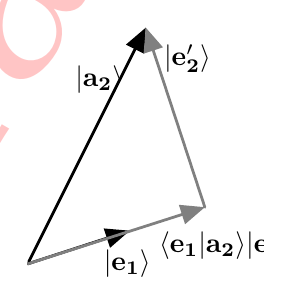
\begin{tikzpicture}[line cap=round,line join=round,>=triangle 45,x=1.5cm,y=1.5cm]
\clip(0,-0.12) rectangle (2,2);
\draw [->,line width=1pt] (0,0) -- (1,2);
\draw [->,line width=1pt] (0,0) -- (0.8640912769793383,0.28106251273126437);
\draw [->,line width=1pt,color=gray] (0,0) -- (1.5,0.48);
\draw [->,line width=1pt,color=gray] (1.5,0.48) -- (1,2);
\draw (0.3201601469559415,1.7592434313457836) node[anchor=north west] {$\mathbf{|a_2\rangle}$};
\draw (0.5615209710734044,0.2038028879947514) node[anchor=north west] {$\mathbf{|e_1\rangle}$};
\draw (1.029326521314053,0.35872384946512484) node[anchor=north west] {$\mathbf{\langle e_1|a_2\rangle |e_1\rangle}$};
\draw (1.0714673610140466,1.9383004752279034) node[anchor=north west] {$\mathbf{|e_2'\rangle}$};
\end{tikzpicture}
\caption{点到线距离}
\end{wrapfigure}
在我准大一暑校学微积分的时候,第一次周测有两个小题-计算点到线和点到面的距离。由于我没有背公式也没有做练习,虽然能够做出点到线这样初中数学题,然而卡在了点到面。于是我便开始任意设定连接点与面向量,从零开始的推导。然而我摆弄了5分钟实在想不通该如何把一个向量投影再平面上,好在鬼使神差地我想到先去用这套推出点到线距离公式看看。我轻松的将设定连接点与线向量$\mathbf{p}$\textbf{运用点乘投影}到线$\mathbf{s}$上。当然首先我们需要让$\mathbf{s}$是只描述\textbf{方向}的单位向量$\mathbf{\^{s}=\frac{s}{|s|},|s|=\sqrt{\mathbf{s}\cdot\mathbf{s}}}$,这样我就能够将$\mathbf{p}$投影在线段的方向上得到$\mathbf{p_l}=(\mathbf{p}\cdot \mathbf{\^{s}})\mathbf{\^{s}}$,使得点到线的距离为\textbf{垂直(正交)于}线的向量$\mathbf{d}=\mathbf{p}-\mathbf{p_l}$,其模长就是答案。\index{格拉姆-施密特正交化}

接下来我顺着这样的思想,首先从平面公式上随便生成两个点得到一个向量$\mathbf{a}$,然后我用其中一个点与目标点形成向量$\mathbf{p}$投影在线上$\mathbf{p_a}=(\mathbf{p}\cdot\mathbf{\^{a})\^{a}}$,不过$\mathbf{p-p_a}$是这条线到点的最短距离。不难想象$\mathbf{p-p_a}$投影在平面上垂直于$\mathbf{a}$,因此我们重复之前操作找到一个垂直于$\mathbf{a}$的向量$\mathbf{o}$,最后我们就能过得到连接目标点到平面的垂直距离为$\mathbf{d}=\mathbf{p-(p\cdot\^{a})\^{a}-(p\cdot\^{o})\^{o}}$。其实在那时我就以及模糊地觉察到了,这样的过程或许可以继续的推广下去。不过鉴于我无法想象一个点到体的距离,因而打消了这样的念头。
\begin{defn}
\textbf{格拉姆-施密特正交化}是用投影的思想通过适当的线性组合将$V$中的任意一组基转换成一组标准正交基的方式。
\end{defn}
假设基底$B=\{|a_i\rangle\}^N_{i=1}$。我们可以对$|a_i\rangle$线性组合得到一组标准正交的向量。首先,我们直接标准化$|a_1\rangle$得到$|e_1\rangle=|a_1\rangle/\sqrt{\langle a_1|a_1\rangle}$使得$\langle e_1|e_1\rangle=1$。接下来我们希望让$|e_2\rangle$正交于$|e_1\rangle$,那么就需要巧妙利用\textbf{点乘投影的思想}。

如图2.1所示,我们将向量$|a_2\rangle$投影在$|e_1\rangle$上面得到$\langle e_1|a_2\rangle |e_1\rangle$,然后我们用$|a_2\rangle$减去其在$|e_1\rangle$上的投影就能够得到一个\textbf{垂直于}$|e_1\rangle$的向量$|e_2'\rangle=|a_2\rangle-\langle e_1|a_2\rangle |e_1\rangle$。我们对其\textbf{归一化}就能够得到单位向量$|e_2\rangle = |e_2'\rangle/\sqrt{\langle e_2'|e_2'\rangle}$。我们固然能够从图上直观的看出$|e_1\rangle$垂直于$|e_2'\rangle$,但还是需要用"代数"推出其\textbf{正交性}有$\langle e_1|e_2'\rangle=\langle e_1|a_2\rangle-\langle e_1|a_2\rangle \langle e_1|e_1\rangle = 0$。

接下来用我们用之前点到面推导的思路,将$|a_3\rangle$减去其在$|e_1\rangle,|e_2\rangle$方向上投影的向量,进而得到
\begin{equation}
|e_3'\rangle = |a_3\rangle-|e_1\rangle\langle e_1|a_3\rangle-|e_2\rangle\langle e_2|a_3\rangle
\end{equation}
,最后我们再对其归一化得到$|e_3\rangle$。不难验证$|e_3'\rangle$是\textbf{正交于}$|e_1\rangle$和$|e_2\rangle$的,$\langle e_1|e_3'\rangle = \langle e_1|a_3\rangle - \langle e_1|e_1\rangle \langle e_1|a_3\rangle - \langle e_1|e_2\rangle \langle e_2|a_3\rangle = 0$,同理有$\langle e_2|e_3'\rangle = 0$。这其中的规律很显然,如果我们已经计算了在该基底上$m$个标准正交向量$|e_1\rangle,\cdots,|e_m\rangle$且$m<N$,那么可以用如下规则计算下一个向量$|e_{m+1}\rangle$:

\begin{align}
|e_{m+1}'\rangle &= |a_{m+1}\rangle - \sum^m_{i=1}|e_i\rangle\langle e_i|a_{m+1}\rangle,\\
|e_{m+1}\rangle &= \frac{|e_{m+1}'\rangle}{\sqrt{\langle e_{m+1}'|e_{m+1}'\rangle}}.
\end{align}\textbf{注意:}除了第一步之外的任意步骤$i$都是需要利用上一步得出的标准正交向量$|e_i\rangle$,因此计算$|e_{m+1}\rangle$需要我们\textbf{重复}上述操作$m$次。此外,每一步骤都是原有向量$|a_{m+1}\rangle$减去基底的\textbf{线性组合}。$\spadesuit$
\subsection{施瓦茨不等式(Schwarz Inequality)}
\textbf{柯西-施瓦茨不等式}是一个在数学上有着广泛应用的很重要的不等式,无论是有限维度还是无限维度它都成立。在二维和三维的情况下,我们能够很直观的想象该等式的描述。因为一个向量投影到另一个向量上的模长一定小于或者等于自身,毕竟$\cos \theta$的最大值是$1$,其中$\theta$为两个向量的夹角。\index{施瓦茨不等式}
\begin{thm}
\textbf{内积空间}$V$上的任意一对向量$|a\rangle,|b\rangle$都有\textbf{施瓦茨不等式}:\\ $\langle a|a\rangle\langle b|b\rangle \geq |\langle a|b\rangle|^2$成立。
\end{thm}
\textbf{证明:}首先,我们需要利用施密特正交化建立$|a\rangle,|b\rangle$之间线性组合的关系。我们让第一个正交标准基为$|e_1\rangle=|a\rangle/\sqrt{\langle a|a\rangle}$,那么就有,
\begin{align}
|e_2\rangle &= |b\rangle - \langle e_1|b\rangle |e_1\rangle=|b\rangle - \frac{\langle a|b\rangle}{\langle a|a\rangle} |a\rangle \Rightarrow|b\rangle = \frac{\langle a|b\rangle}{\langle a|a\rangle} |a\rangle + |e_2\rangle \\
\langle b|b\rangle &= \left|\frac{\langle a|b\rangle}{\langle a|a\rangle} \right| ^2\langle a|a\rangle + \langle e_2|e_2\rangle = \frac{|\langle a|b\rangle|^2}{\langle a|a\rangle} + \langle e_2|e_2\rangle\\
\langle e_2|e_2\rangle &\geq 0 \Rightarrow \langle b|b\rangle\geq \frac{|\langle a|b\rangle|^2}{\langle a|a\rangle} \Rightarrow \langle a|a\rangle\langle b|b\rangle \geq |\langle a|b\rangle|^2. \rm(Q.E.D)
\end{align}等式成立当且仅当$\langle e_2|e_2\rangle = 0 \Rightarrow |e_2\rangle =|b\rangle - \frac{\langle a|b\rangle}{\langle a|a\rangle} |a\rangle = 0$,也就是当$|a\rangle,|b\rangle$成\textbf{正比}(线性相关夹角为零)时。这样抽象的推导使得施瓦茨不等式可以被广泛的运用,因为我们仅仅只从的内积空间的基本假设推导出了施瓦茨不等式,而\textbf{没有}用到
内积的特殊性质。因此,每当我们遇到一个新的内积空间时,我们不需要再证明这个不等式。
\subsection{向量的模长}
中学在处理平面或空间中的有向线段等物体时,我们可以用向量长度的直观概念来定义\textbf{点乘}。这里我们先引入内积,然后再来定义向量的长度。
\begin{defn}
内积空间中的一个向量$|a\rangle$的\textbf{范数(norm)}\index{范数(norm)},也就是长度定义为$\|a\|\equiv \sqrt{\langle a|a\rangle}$。向量$\alpha|a\rangle +\beta|b\rangle$的模记作$\|\alpha a+
\beta b\|$。
\end{defn}
\textbf{向量的范数有以下3条性质:}\\
  \textbf{1. 范数正定性:} $\|a\|\geq 0$并且$\|a\|=0$当且仅当$|a\rangle = |0\rangle$。\\
  \textbf{2. 齐次性:}$\|\alpha a\|=|\alpha|\|a\|$; \textbf{3. 三角不等式:}$ \|a+b\|\leq \|a\|+\|b\|$。

向量空间上任何满足上述性质的\textbf{函数}称为\textbf{范数},\textbf{赋范线性空间(normed linear space)}\index{赋范线性空间}是定义了范数的向量空间。因此,我们并不需要内积也能够有范数。在赋范线性空间中我们可以引入两个向量之间的“距离”这样的概念。向量$|a\rangle,|b\rangle$之间的距离记作并定义为$d(a,b)\equiv\|a-b\|$。不难发现它满足之前\textbf{度量函数}的全部性质。不过,我们并不需要用赋范线性空间来定义距离。比如,我们可以定义球面上的两个点的距离,但不需要定义两个点的加法,也就是向量空间所必须要的结构没有定义,因此球面的点形成了度量空间,但不是线性空间。
\begin{thm}
\textbf{范数线性空间}是\textbf{内积空间}当且仅当其范数满足\textbf{平行四边形定律}。
\end{thm}

内积空间都自然是赋范线性空间,不过反之则不成立。也就是满足上述性质的空间一定是内积空间,但是如果其范数满足\textbf{平行四边形法则(parallelogram law)}\index{平行四边形法则}:$\|a+b\|^2+\|a-b\|^2=2\|a\|^2+2\|b\|^2$,那么我们就可以在该空间上定义内积: $\langle a|b\rangle \equiv \frac{1}{4}\{\|a+b\|^2-\|a-b\|^2 - i(\|a+ib\|^2-\|a-ib\|^2)\}$

\begin{thm}
所有\textbf{有限维度}向量空间都可以被转变为一个\textbf{内积空间}。
\end{thm}

设$V$为$N$维度向量空间,有一组基$\{a_i\}^N_{i=1}$对于任意向量$|a\rangle$的分量为$\{\alpha_i\}^N_{i=1}$,也就是$|a\rangle = (\alpha_1,\cdots,\alpha_N)$。我们定义范数:$\|a\|^2=\sum^N_{i=1}|\alpha_i|^2$,不难验证其满足平行四边形法则。比如,我们考虑线性空间$\mathbb{C}^n$中两个向量$|a\rangle,|b\rangle$之间的距离:
\begin{equation}
    d(a,b)=\|a-b\|=\sqrt{\langle a-b|a-b\rangle}=\sqrt{\sum^n_{i=1}|\alpha_i-\beta_i|^2}.
\end{equation}
我们还可以定义另一个范数,$\|a\|_1 \equiv \sum_{i=1}^n|\alpha_i|$并得到距离,$d_1(a,b)=\|a-b\|_1=\sum_{i=1}^n|\alpha_i-\beta_i|$。实际上这两个范数都是以下范数和距离函数在$p=2$和$p=1$的特殊情况:
\begin{align}
    \|a\|_p &\equiv \left(\sum_{i=1}^n|\alpha_i|^p\right)^{1/p}\\
    d(a,b)_p &=\|a-b\|_p=\left(\sum^n_{i=1}|\alpha_i-\beta_i|^p\right)^{1/p}.
\end{align}
\section{线性映射(Linear Maps)}
尽管我们以及为线性空间增添了\textbf{内积}和\textbf{范数}这些结构,但是我们仍旧还是在单一的向量空间进行讨论。因此,若要带来更加广泛和重要的运用,我们需要让一个向量空间能够变换和联系到另一个向量空间且保持向量加法和标量乘法。这样的操作被称之为\textbf{线性映射(linear maps)}\index{线性映射(linear maps)}或者\textbf{线性变换(linear transformation)}\index{线性变换(linear transformation)}。我们先来用几个例子回顾之前学习的\textbf{映射}。
\begin{exmp}
\textbf{1.} 设映射$F:\mathbb{R}^2\xrightarrow{}\mathbb{C}$有$F(x,y)=U(x,y)+iV(x,y)$且$U:\mathbb{R}^2\xrightarrow{}\mathbb{R},V:\mathbb{R}^2\xrightarrow{}\mathbb{R}$。设映射$f:\mathbb{R}^2\xrightarrow{}\mathbb{R}$有$f(x)=(x-2,3x-4)$。\\
\textbf{2.} 空间中质点的运动可以看作是映射$
M:[a,b]\xrightarrow{}\mathbb{R}^3$,其中$[a,b]$是描述时间的实闭区间,有任意时刻$t\in[a, b]$。我们定义$M(t)=(x(t),y(t),z (t))$,其中$x(t),y(t),z (t)$都是关于$t$的实值函数。这样$M(t)$就是描述质点运动路径以时间为变量的函数,其中$a$和$b$分别是开始和结束的时刻。
\end{exmp}
\begin{defn}
复向量空间$V,W$之间的\textbf{线性映射}$\mathbf{T}:V\xrightarrow{}W$需要满足:
\begin{equation}
    \mathbf{T}(\alpha|a\rangle+\beta|b\rangle)=\alpha\mathbf{T}(|a\rangle)+\beta\mathbf{T}(|b\rangle),\ \forall |a\rangle,|b\rangle\in V \land \alpha,\beta \in \mathbb{C}.
\end{equation}
线性变换$T: V\xrightarrow{}V$称为$V$的\textbf{自同态(endomorphism)}\index{自同态(endomorphism)}或$V$上的\textbf{线性算子(linear operator)}\index{线性算子(linear operator)}。对一个向量的记法可省略括号:$\mathbf{T}(|a\rangle)\equiv\mathbf{T}|a \rangle$。同样的定义也适用于实向量空间,注意两个向量空间一定有同一标量域。
\end{defn}

由定义可得\textbf{线性映射}$\mathbf{T}:V\xrightarrow{}W$有以下性质:
\textbf{1.} $\mathbf{T}|0\rangle_V=|0\rangle_W.$ 比如$f(x)=x+3$就不是线性映射。
\textbf{2.} 若$|v_1\rangle,|v_2\rangle,\cdots,|v_n\rangle\in V$线性相关,则$\mathbf{T}|v_1\rangle,\mathbf{T}|v_2\rangle,\cdots,\mathbf{T}|v_n\rangle$线性相关,然反之则非也。
\textbf{3.} 若有限维的$V$中的一组基底为$B=\{|a_i\rangle\}^N_{i=1}$则对任意的$|v\rangle \in V$都有$|v\rangle = \sum^N_{i=1}\alpha_i|a_i\rangle$使得$\mathbf{T}|v\rangle =\sum^N_{i=1}\alpha_i\mathbf{T}|a_i\rangle$。
\begin{defn}
映射$f:V\xrightarrow{}W$是\textbf{反线性(antilinear)}\index{反线性(antilinear)}(或\textbf{共轭线性}或\textbf{半线性})映射则有:$f(\alpha a+\beta b)=\alpha^*f(a)+\beta^*f(b)$。
\end{defn}

从$V$到$W$的不同线性映射组成的集合记作$L(V,W)$,\textbf{集合$L(V,W)$是一个向量空间}。\textbf{零变换}$\mathbf{0}$是对每一个$V$中向量都映射到$W$中的零向量上。线性变换$\mathbf{T,U}$的\textbf{加法}为线性变换$\mathbf{T+U}$,其对向量$|a\rangle \in V$有操作定义为$\mathbf{T+U}|a \rangle \equiv \mathbf{T}|a\rangle + \mathbf{U}|a\rangle$。类似地,定义\textbf{标量乘法}$\alpha\mathbf{T}$有$(\alpha\mathbf{T})|a\rangle\equiv\alpha(\mathbf{T}|a\rangle)=\alpha\mathbf{T}|a\rangle$。$V$的\textbf{自同态}的集合用$L(V)$或$\rm End(V)$表示,而不是$L(V,V)$。

\begin{defn}
设$V$和$U$为内积空间,线性映射$\mathbf{T}:
V\xrightarrow{}U$称为\textbf{等距映射(isometric map)}\index{等距映射(isometric map)}如有:$\langle \mathbf{T}a|\mathbf{T}b\rangle = \langle a|b\rangle, \ \forall |a\rangle,|b\rangle\in V.$
\end{defn}

如果有$U = V$,则$\mathbf{T}$称为\textbf{线性等距(linear isometry)}\index{线性等距(linear isometry)}或$V$的等距。我们通常将复(实)内积空间$V$的等距称为\textbf{酉(unitary)}\index{酉(unitary)}(正交)线性算子。
\begin{exmp} \textbf{线性映射的例子:}
\begin{enumerate}
\item 设$V$是一维空间(如$V = \mathbb{C}$),则$V$的任意自同态$\mathbf{T}$的形式为$\mathbf{T}|x\rangle = \alpha|x\rangle$,其中$\alpha$为标量。如果$\mathbf{T}$是等距,则有$|\alpha|^2 = 1$。如果$V=\mathbb{R}$且$\mathbf{T}$是等距,则有$\mathbf{T}|x\rangle =\pm|x\rangle$。
\item 设双射函数$\pi:\mathbb{N}\xrightarrow{}S$为$S=\{1,2,\cdots,n\}$上的任意一个\textbf{排列(permutation)}\index{排列(permutation)}。也就是说$\pi$会任意打乱(赋予)$S$一个顺序,那么对于$|a\rangle=(\alpha_1,\alpha_2,\cdots,\alpha_n)\in\mathbb{C}^n$就有\textbf{线性映射}$\mathbf{A}_\pi|a\rangle=(\alpha_{\pi(1)},\alpha_{\pi(2)},\cdots,\alpha_{\pi(n)})$。
\item 任意的多项式向量$|x\rangle\in \mathcal{P}^c[t]$有$x(t)=\sum_{j=0}^n\alpha_jt^j$,定义$\mathbf{D}|x\rangle = |x_d\rangle, \ x_d(t)=\sum_{j=1}^n k\alpha_jt^{j-1}$,那么线性映射$\mathbf{D}$称作\textbf{导数算子(derivative operator)}\index{导数算子(derivative operator)}。若定义$\mathbf{S}|x\rangle = |x_s\rangle,\ x_s(t)=\sum_{j=0}^n [\alpha_j/(k+1)]t^{j=1}$,那么线性映射$\mathbf{S}$称作\textbf{积分算子(integration operator)}\index{积分算子(integration operator)}。
\item 设$\mathcal{C}^n(a,b)$为闭区间$[a,b]$上$n$阶可导且连续的所有实值函数,对于任意$|f\rangle\in \mathcal{C}^n(a,b)$定义$\mathbf{G}|f\rangle=|u\rangle, \ u(t)=g(t)f(t)$,其中$g(t)$为$\mathcal{C}^n(a,b)$中一个固定的函数,那么$\mathbf{G}$为线性映射。
\end{enumerate}
\end{exmp}

由之前的性质3可知:两个线性变换$\mathbf{T}: V\xrightarrow{}W$和$\mathbf{U}: V\xrightarrow{}W$是相等的当且仅当对于所有$V$基底中的$|a_i\rangle$都有$\mathbf{T}|a_i\rangle = \mathbf{U}|a_i\rangle$成立。
因此,一个线性变换是由它在其定义域上的某一组基底所唯一决定的。对于内积空间来说我们还可以用其他更方便的方法来定义线性算子的相等。
\begin{thm}
内积空间的自同态$\mathbf{T}$为零变换$\mathbf{0}$当且仅当$\langle b|\mathbf{T}a\rangle=0,\forall |a\rangle,|b\rangle$。
\end{thm}
\textbf{证明:}如果$\mathbf{T=0}$那么显然就有$\langle b|\mathbf{T}a\rangle=0$,当且仅当需反之亦然。因此,如果$\langle b|\mathbf{T}a\rangle=0$并且定义映射$|b\rangle=\mathbf{T}|a\rangle$,那么根据内积的正定性就有,$\langle \mathbf{T}a|\mathbf{T}a\rangle=0\Leftrightarrow\mathbf{T}|a\rangle=0\Leftrightarrow\mathbf{T}=0,\ \forall |a\rangle$。$\clubsuit$
\begin{thm}
内积空间的自同态$\mathbf{T}$为零变换$\mathbf{0}$当且仅当$\langle a|\mathbf{T}a\rangle=0,\forall |a\rangle$。
\end{thm}
\textbf{证明:}如果$\mathbf{T=0}$那么$\langle a|\mathbf{T}a\rangle=0$,反之如果$\langle a|\mathbf{T}a\rangle=0,\forall |a\rangle$且设$|c\rangle = \alpha|a\rangle+\beta|b\rangle$则有$\langle c|\mathbf{T}c\rangle=\langle \alpha a+\beta b|\mathbf{T}|\alpha a+\beta b\rangle=0$,引入\textbf{极化恒等式(polarization identity)}\index{极化恒等式(polarization identity)}:
\begin{equation}
\alpha^*\beta\langle a|\mathbf{T}b\rangle+\alpha\beta^*\langle b|\mathbf{T}a\rangle=\langle c|\mathbf{T}c\rangle-|\alpha|^2\langle a|\mathbf{T}a\rangle-|\beta|^2\langle b|\mathbf{T}b\rangle
\end{equation}根据定理$\langle a|\mathbf{T}a\rangle=\langle b|\mathbf{T}b\rangle=\langle c|\mathbf{T}c\rangle=0$使得$\alpha^*\beta\langle a|\mathbf{T}b\rangle+\alpha\beta^*\langle b|\mathbf{T}a\rangle=0$。引用定理2.3.1: $\langle b|\mathbf{T}a\rangle=0,\forall |a\rangle,|b\rangle\Leftrightarrow\mathbf{T}=0,\ \forall |a\rangle$使得前后一致。$\clubsuit$

为了证明内积空间上的两个算子$\mathbf{T}$和$\mathbf{U}$是相等的,我们可以让它们作用于任意向量并证明它们会得到同样的结果$\langle a|\mathbf{T}b\rangle=\langle a|\mathbf{U}b\rangle,\forall |a\rangle,|b\rangle$,或者用上述定理来证明$\mathbf{T-U}$是零变换$\mathbf{0}$,$\langle a|\mathbf{T-U}|b\rangle=0,\forall |a\rangle,|b\rangle$。
\begin{defn}
\textbf{极化恒等式}用赋范向量空间的\textbf{范数}表示两个向量的\textbf{内积}。
\end{defn}
首先,考虑实向量空间有满足平行四边形法则的范数,
\begin{align}
     \|a+b\|^2&=\|a\|^2+2\langle a| b\rangle+\|b\|^2 
\end{align}
\begin{align}
    \langle a| b\rangle &= \frac{1}{2}(\|a+b\|^2-\|a\|^2-\|b\|^2)\\
     &= \frac{1}{2}(\|a\|^2+\|b\|^2-\|a-b\|^2)\\
     &= \frac{1}{4}(\|a+b\|^2-\|a-b\|^2)
\end{align}
式2.43就是我们常见的一个极化恒等式,实际上我们还可以用点乘定义范数$\|a+b\|^2=\|a\|^2+2\langle a| b\rangle+\|b\|^2,\|a-b\|^2=\|a\|^2-2\langle a| b\rangle+\|b\|^2$\textbf{两式相减}得到极化恒等式,或者\textbf{两式相加}得到平行四边形法则。

我们顺着之前的结果得到,$\langle a|b\rangle+\langle b|a\rangle= \frac{1}{2}(\|a+b\|^2-\|a-b\|^2)$。注意根据复内积的定义$\langle a|b\rangle\in\mathbb{C}$,$\langle a|b\rangle$有虚数部分,由于$\langle a|b\rangle=\langle b|a\rangle^*$使得$\langle a|b\rangle+\langle b|a\rangle$正好抵消了各自的虚数部分,好在这也告诉我们它们的实数部分相等,也就是有$\mathfrak{Re}\langle a|b\rangle= \frac{1}{4}(\|a+b\|^2-\|a-b\|^2)$。接下来,我们还需要找到虚数部分。既然$\mathfrak{Im}(\langle a|b\rangle+\langle b|a\rangle)=0$,那么$\mathfrak{Im}(\langle a|b\rangle-\langle b|a\rangle)=2\mathfrak{Im}(\langle a|b\rangle)$。找到$\langle a|b\rangle-\langle b|a\rangle$只需用对之前\textbf{两式相减}得到极化恒等式稍作修改:
\begin{align}
    \langle a+ib|a+ib\rangle&=\langle a|a\rangle+\langle ib|a\rangle+\langle a|ib\rangle + \langle b|b\rangle\\
    \|a+ib\|^2 &= \|a\|^2-i\langle b|a\rangle+i\langle a|b\rangle+\|b\|^2\\
    \|a-ib\|^2 &= \|a\|^2+i\langle b|a\rangle -i\langle a|b\rangle+\|b\|^2\\
    \|a+ib\|^2-\|a-ib\|^2&=2i(\langle a|b\rangle-\langle b|a\rangle)\\
    \langle a|b\rangle-\langle b|a\rangle&=-\frac{1}{2}i(\|a+ib\|^2-\|a-ib\|^2)
\end{align}
这样我们找到了$\mathfrak{Im}(\langle a|b\rangle)=-\frac{1}{4}(\|a+ib\|^2-\|a-ib\|^2)$,最后结合实部:
\begin{align}
	\langle a|b\rangle \equiv \frac{1}{4}\{\|a+b\|^2-\|a-b\|^2 - i(\|a+ib\|^2-\|a-ib\|^2)\}
\end{align}
这里的符号确实有些歧义,$a,b$在这里都是向量,而不是我们所习惯的实数,所以$\langle a+ib|a+ib\rangle=\|a+ib\|^2$而不能取共轭$\langle a+ib|a-ib\rangle$。此外,或许大家注意到我们推导出来的式2.49与大多数学书上的极化恒等式不同,并且恰好是它们的共轭。这是由于物理约定左矢,也就是第一位\textbf{自变量(argument)}\index{自变量(argument)}取共轭,数学上一般在第二位取共轭。

\subsection{线性映射的核(kernel)}
从线性映射的定义中可以直接得出性质1: $V$中的零向量的像也是$W$中的零向量$\mathbf{T}|0\rangle_V=|0\rangle_W$。这对一般映射并不成立,不过对线性映射是一定成立的。$V$中的其他向量也能够映射到$W$的零向量上,有如下定理:
\begin{thm}
若$V$中的向量组成的一个集合在线性变换$\mathbf{T}:V\xrightarrow{}W$下都映射到了$W$的零向量上,那么该集合形成了$V$的子空间称为$\mathbf{T}$的\textbf{核(kernel)}\index{核(kernel)},或\textbf{零空间(null space)}\index{零空间(null space)},记作$\ker\mathbf{T}=\{|v\rangle \in V:\mathbf{T}|v\rangle=|0\rangle_W\}$。$\ker\mathbf{T}$的维度称作$V$的\textbf{零化度(nullity)}\index{零化度(nullity)}。
\end{thm}
\textbf{证明:} 设$|a\rangle,|b\rangle\in\ker\mathbf{T}$则$\mathbf{T}|a\rangle=\mathbf{T}|b\rangle=|0\rangle_W$使$\mathbf{T}(\alpha|a\rangle+\beta|b\rangle)=\alpha\mathbf{T}(|a\rangle)+\beta\mathbf{T}(|b\rangle)=|0\rangle_W$,有$\alpha|a\rangle+\beta|b\rangle\in\ker\mathbf{T}$。$\clubsuit$
\begin{thm}
线性映射$\mathbf{T}:V\xrightarrow{}W$的值域$\mathbf{T}(V)$是$W$的子空间(证明思路如上)。我们将$\mathbf{T}(V)$的维数称为$\mathbf{T}$的\textbf{秩(rank)}\index{秩(rank)}。
\end{thm}
\begin{thm}
线性映射$\mathbf{T}$为单射当且仅当其核为零向量$\ker\mathbf{T}=\{|0\rangle\}$。
\end{thm}
\textbf{证明:}假设$|v_1\rangle,|v_2\rangle\in V$有同一个像$\mathbf{T}|v_1\rangle=\mathbf{T}|v_2\rangle
$,那么意味$\mathbf{T}(|v_1\rangle-|v_2\rangle)=|0\rangle_W$如果核为零向量,那么$|v_1\rangle=|v_2\rangle$使得该映射一定为单射。$\clubsuit$
\begin{thm}
线性\textbf{等距映射}$\mathbf{T}$一定是单射的。
\end{thm}
\textbf{证明:}设$\mathbf{T}$为等距映射且$\forall|a\rangle,|b\rangle\in\ker\mathbf{T}$则有$\langle a|b\rangle=\langle\mathbf{T}a|\mathbf{T}b\rangle=\langle 0|0 \rangle = 0$。由内积性质可得$|a\rangle=|b\rangle=|0\rangle_V$,由定理2.3.5得$\mathbf{T}$为单射。$\clubsuit$
\begin{thm}
对于任意线性映射$\mathbf{T}:V\xrightarrow{}W$都有\textbf{秩-零化度定理(Rank–nullity theorem)}\index{秩-零化度定理}或维度定理(dimension theorem)\index{维度定理(dimension theorem)}:
\begin{equation}
    \dim V=\dim\ker\mathbf{T}+\dim\mathbf{T}(V)
\end{equation}
\end{thm}
\textbf{证明:}设$V$的一组基为$B=\{|a_1\rangle,|a_2\rangle,\cdots,|a_n\rangle\}$且$\ker\mathbf{T}$的一组基为$B'=\{|a_1\rangle,|a_2\rangle,\cdots,|a_k\rangle\}$。对于任意$|v\rangle\in V$都有$\mathbf{T}|v\rangle=\mathbf{T}\sum^n_{i=1}\alpha_i|a\rangle_i$。其求和中的前$k$项都是\textbf{核}中的基,因此$\mathbf{T}\alpha_1|a\rangle_1=\mathbf{T}\alpha_2|a\rangle_2=\cdots=\mathbf{T}\alpha_k|a\rangle_k=0$。也就是意味着,$\mathbf{T}(V)$的一组基为$\{\mathbf{T}|a_{k+1},\cdots,\mathbf{T}|a_{n}\}$使得$\dim\mathbf{T}(V)=n-k,\dim V=n,\dim\ker\mathbf{T}=k$。$\clubsuit$
\begin{thm}
有限维向量空间的\textbf{自同态}是双射,如果其为单射或满射。
\end{thm}
\textbf{证明:}引理2.3.5单射映射当且仅当核为零向量使得引理2.3.7有$\dim V=\dim\mathbf{T}(V)$,单射且基数相同则等价于双射。然后自同态若是满射则直接可得$\dim V=\dim\mathbf{T}(V)$。$\clubsuit$\textbf{注意:}维度定理只对有限维向量空间有效。$\spadesuit$
\begin{exmp}
设$\mathbf{T}:\mathbf{R}^4\xrightarrow{}\mathbf{R}^3$给定$\mathbf{T}(x_1,x_2,x_3,x_4)=(2x_1 + x_2 + x-3−x_4,x_1 + x_2 + 2x_3 + 2x_4,x_1−x_3−3x_4)$。首先,我们先来计算$\ker\mathbf{T}$:
\begin{align}
    \mathbf{T}(x_1,x_2,x_3,x_4)&=(0,0,0)\\
    2x_1 + x_2 + x-3−x_4&=0\\
    x_1 + x_2 + 2x_3 + 2x_4&=0\\
    x_1−x_3−3x_4&=0
\end{align}
该方程的“解”为:$x_1=x_3 + 3x_4;x_2 = − 3x_3 − 5x_4$。因此,若要在$\ker\mathbf{T}$中,其向量必须是$\mathbb{R}^4$的形式:$(x_3 + 3x_4,−3x_3 − 5x_4,x_3,x_4) = x_3(1,−3,1,0)+ x_4(3,−5,0,1)$。其中$x_3,x_4$为任意实数,使得任意$\ker\mathbf{T}$中的向量都是两个线性无关的向量$(1,−3,1,0),(3,−5,0,1)$的线性组合。因此有$\dim\ker\mathbf{T}=2$。根据定理2.3.7有$\dim\mathbf{T}(\mathbb{R}^4)=2$,注意到:$\mathbf{T}(x_1,x_2,x_3,x_4)=(2x_1 + x_2 + x-3−x_4)(1,0,1)+(x_1 + x_2 + 2x_3 + 2x_4)(0,1,-1)$。因此,任意$\mathbf{T}(x_1,x_2,x_3,x_4)\in\mathbf{T}(\mathbb{R}^4)$都可以写作两个线性无关的向量$(1,0,1),(0,1,-1)$。
\end{exmp}
\subsection{线性同构(Linear Isomorphism)}
\begin{defn}
向量空间$V$是\textbf{同构的(isomorphic)}\index{同构的(isomorphic)}$W$记作$V\cong W$,$\mathbf{T}$是\textbf{同构(isomorphism)}\index{同构(isomorphism)}若存在一个双射线性映射$\mathbf{T}:V\xrightarrow{}W$或者说\textbf{可逆(invertible)}\index{可逆(invertible)}线性映射。一个双射的自同态$\mathbf{T}:V\xrightarrow{}V$称之为$V$的\textbf{自同构(automorphism)}\index{自同构(automorphism)}。$V$的自同构集和记作$GL(V)$。
\end{defn}

在许多情况下,两个向量空间虽然“看似”不同,但实际上它们非常相似。例如,实数域上的二维向量空间$\mathbb{C}$就像是线性空间$\mathbb{R}^2$。广义上来说就是,域$\mathbb{F}$上的$n$维向量空间类似于向量空间$\mathbb{F}^n$。上述定义的\textbf{同构}就是描述相似性的普遍抽象性质。

映射$\mathbf{T}:\mathbb{C}\xrightarrow{}\mathbb{R}^2,\mathbf{T}(x+iy)=(x,y)$是同构,不难验证首先$\mathbf{T}$是线性映射,然后其为单射,最后是满射。不过我们需要特别\textbf{注意:}集合$\mathbb{C}$和$\mathbb{R}^2$是同构的,仅在其\textbf{结构(structure)}\index{结构(structure)}都为线性空间下成立,如果我们考虑其他结构,则它们可能不是同构的。比如,$\mathbb{C}$的元素有乘法,但是$\mathbb{R}^2$没有。
\begin{thm}
有限维向量空$V$的\textbf{等距}是该向量空间的\textbf{自同构}。
\end{thm}
\textbf{证明:}根据定义2.3.3,$V$的\textbf{等距}$\mathbf{T}$既是自同态也是等距映射。定理2.3.6得到$\mathbf{T}$作为等距映射是单射,定理2.3.8得到自同态$\mathbf{T}$是双射的,因而根据定义2.3.5可得$\mathbf{T}$也是\textbf{自同构}。$\clubsuit$
\begin{thm}
\textbf{满射}线性映射$\mathbf{T}:V\xrightarrow{}W$是\textbf{同构}当且仅当其\textbf{零化度}为零。
\end{thm}
\textbf{证明:}因为$\ker\mathbf{T}=\{|0\rangle_V\}$,定理2.3.5可得$\mathbf{T}$是单射,使得$\mathbf{T}$为既是单射又是满射的双射线性映射也就是\textbf{同构}。$\clubsuit$
\begin{thm}
\textbf{单射}线性映射$\mathbf{T}:V\xrightarrow{}W$将一组线性无关的向量对应到另一组线性无关的向量上。
\end{thm}
\textbf{证明:}由单射可得如果$\mathbf{T}|a\rangle=\mathbf{T}|b\rangle$,则$|a\rangle=|b\rangle$。因此有$\alpha_1|a_1\rangle+\alpha_2|a_2\rangle+\cdots+\alpha_n|a_n\rangle=0 \Leftrightarrow \alpha_1\mathbf{T}|a_1\rangle+\alpha_2\mathbf{T}|a_2\rangle+\cdots+\alpha_n\mathbf{T}|a_n\rangle=0, \alpha_1=\cdots=\alpha_n=0$,使得$|a_1\rangle,|a_2\rangle,\cdots,|a_n\rangle$线性无关当且仅当$\mathbf{T}|a_1\rangle,\mathbf{T}|a_2\rangle,\cdots,\mathbf{T}|a_n\rangle$。$\clubsuit$
\begin{thm}
两个有限维向量空间$V,W$是同构的,\textbf{当且仅当}它们具有\textbf{相同}的维数$\dim V = \dim W$。
\end{thm}
\textbf{证明:}设有限维空间$V,W$有$\dim V =\dim W =n$,则$V$的一组基为$B_V=\{|a_i\rangle\}^n_{i=1}$,$W$的一组基为$B_w=\{|b_i\rangle\}^n_{i=1}$。使得$V$中不同的向量$|v\rangle$都能唯一的对应到$W$中的不同向量。因此$\mathbf{T}:V\xrightarrow{}W$一定是\textbf{双射}。$\clubsuit$

到这里,我们终于验证了一开始所说的相似性就是同构。因此,\textbf{域$\mathbb{F}$上的$n$维向量空间与向量空间$\mathbb{F}^n$是同构的}。也就是,所有的$\mathbb{R}$上的$n$为向量空间和$\mathbb{R}^n$都是同构的。
\begin{thm}
设$V = V_1\oplus V_2$且$\mathbf{T}$是$V$的\textbf{自同构},使$V_1$为\textbf{不变量(invariant)}\index{不变量(invariant)},即$\mathbf{T}(V_1) = V_1$,那么$V_2$也是不变量。实际上,只要有一个是不变量,则另一个也是不变量。
\end{thm}
\textbf{证明:}$V_1\oplus V_2=\mathbf{T}(V)=\mathbf{T}(V_1\oplus V_2)=\mathbf{T}(V_1)\oplus\mathbf{T}(V_2)=V_1\oplus \mathbf{T}(V_2)$由定理2.1.11可得$\mathbf{T}(V_2)=V_2$。$\clubsuit$
\begin{exmp}\textbf{维度定理的另一个证明:}\end{exmp}

设$\mathbf{T}':V\xrightarrow{}W$为线性映射且$\mathbf{T}':V/\ker\mathbf{T}\xrightarrow{}\mathbf{T}(V)$。如果$|a\rangle$为\textbf{等价类}$[a]$的\textbf{代表},则$\mathbf{T}'([a])=\mathbf{T}|a\rangle$。\begin{defn}
若$f$\textbf{定义良好(well defined)}\index{定义良好(well defined)}则有$x=y\Rightarrow(x)=f(y)$。
\end{defn}首先,该映射是有\textbf{定义良好}的,因为如果$[a']=[a]$则有$|a'\rangle=|a\rangle+|z\rangle$其中$|z\rangle\in\ker\mathbf{T}$使得$\mathbf{T'}([a'])\equiv\mathbf{T}|a'\rangle=\mathbf{T}(|a\rangle+|z\rangle)=\mathbf{T}|a\rangle+\mathbf{T}|z\rangle=\mathbf{T}|a\rangle$。

接下来,我们证明$\mathbf{T'}$是一个\textbf{同构}。首先,因为$\mathbf{T}$是线性映射,所以有 $\mathbf{T'}(\alpha[a]+\beta[b])\equiv\mathbf{T}(\alpha|a\rangle+\beta|b\rangle)=\alpha\mathbf{T}(|a\rangle)+\beta\mathbf{T}(|b\rangle)=\alpha\mathbf{T'}([a])+\beta\mathbf{T'}([b])$
使得$\mathbf{T'}$是线性映射。然后,对于任意的$|x\rangle\in\mathbf{T}(V)$,都存在$|y\rangle\in V$使得$|x\rangle=\mathbf{T}|y\rangle=\mathbf{T'}([y])$,因此$\mathbf{T'}$为\textbf{满射}。最后,如果$\mathbf{T'}([x])=\mathbf{T'}([y])$,则意味着$\mathbf{T}|x\rangle=\mathbf{T}|y\rangle$,也就是$\mathbf{T}(|x\rangle-|y\rangle)=0$,那么有$|x\rangle-|y\rangle\in\ker\mathbf{T}$使得$[x]=[y]$,因此$\mathbf{T'}$为\textbf{单射}。因此得到了$\mathbf{T'}$是一个\textbf{同构},根据定理2.4.4:$\dim(V/\ker\mathbf{T})=\dim\mathbf{T}(V)\Leftrightarrow\dim(V)=\dim\ker\mathbf{T}+\dim\mathbf{T}(V)$(Q.E.D)。

\begin{thm}
设$V,W$为线性空间且有线性映射$\mathbf{T}:V\xrightarrow{}W$。若$U$为$V$的子空间,定义$\mathbf{T}':V/U\xrightarrow{}\mathbf{T}(V)$有$\mathbf{T'}([a])=\mathbf{T}|a\rangle$,其中$|a\rangle$为$[a]$的代表,则$\mathbf{T'}$是一个定义良好的\textbf{同构}。
\end{thm}
设$U,V,W$为复向量空间且定义线性映射如下:
\begin{align}
    \mathbf{T}:(U\oplus V)\otimes W \xrightarrow{}(U\otimes W)\oplus(V\otimes W)\\
    \mathbf{T}((|u\rangle+|v\rangle)\otimes|w\rangle)=|u\rangle\otimes |w\rangle+|v\rangle\otimes|w\rangle.
\end{align}
不难看出$\mathbf{T}$是\textbf{同构},因此有$(U\oplus V)\otimes W \cong (U\otimes W)\oplus(V\otimes W)$。这里我们固然可以一如既往繁琐的证明,但用定理2.4.4就要容易的多。根据定理2.1.8和2.1.12可得:
\begin{align}
\dim ((U\oplus V)\otimes W) &= \dim(U\oplus V)\dim\\
&=(\dim U + \dim V)\dim W
\end{align}
\begin{align}
&= \dim U\dim W +\dim V\dim W \\
&= \dim((U\otimes W)\oplus(V\otimes W))
\end{align}
\section{复结构(Complex Structures)}
到目前为止,我们处理向量空间都避免改变其标量的性质。当向量空间是复数时,我们始终保持这个向量空间的标量作为复数。在这部分中,我们将探讨改变标量的可能性,以及随之而来的在向量空间的其他结构中可能发生的相应变化。推广内积的概念能够方便我们讨论关于改变标量以及其他的形式化内容。虽然正确定性的概念对于内积的物理应用是至关重要的,但它的限制性太大,所以我们放宽这个要求,重新定义内积。
\begin{defn}
设$\mathbb{F}$非$\mathbb{C}$即$\mathbb{R}$,则一个域$\mathbb{F}$下的线性空间$V$之上的\textbf{内积}为线性映射$g:V\times V\xrightarrow{}\mathbb{F}$满足如下性质:\\
\textbf{1.}\textbf{对称性(symmetry)}\index{对称性(symmetry)}:$g(|a\rangle,|b\rangle)=g(|b\rangle,|a\rangle)$\\
\textbf{2.}\textbf{双线性(bilinearity)}\index{双线性(bilinearity)}:$g(\alpha|a\rangle+\beta|b\rangle,|c\rangle)=\alpha g(|a\rangle,|c\rangle)+\beta g(|b\rangle,|c\rangle);$\\$空\qquad\qquad\qquad\qquad\qquad\quad \ \, g(|c\rangle,\alpha|a\rangle+\beta|b\rangle)=\alpha g(|c\rangle,|a\rangle)+\beta g(|c\rangle,|b\rangle)$\\
\textbf{3.}\textbf{非退化(non-degeneracy)}\index{非退化(non-degeneracy)}:$g(|a\rangle,|b\rangle)=0,\ \forall|a\rangle\in V \Rightarrow |a\rangle=|0\rangle$
\end{defn}

我们也可以用狄拉克符号$\langle\cdot|\cdot\rangle_{\mathbb{F}}$来表示域$\mathbb{F}$上的内积,当$\mathbb{F}=\mathbb{R}$时,则$\langle\cdot|\cdot\rangle_{\mathbb{F}}=\langle\cdot|\cdot\rangle$。\textbf{非退化}也就是,对于任意的非零向量$|a\rangle\in V$一定都至少存在一个向量$|b\rangle\in V$使得$g(|a\rangle,|b\rangle)\neq 0$。也就是说,仅只有零向量正交于内积空间的所有向量。
\begin{defn}
线性算子$\mathbf{A}\in\rm End(V)$的\textbf{伴随(adjoint)}\index{伴随(adjoint)}记作$\mathbf{A}^T$,满足:
\begin{equation}
    \langle\mathbf{A}a|b\rangle_\mathbb{F}=\langle a|\mathbf{A}^T b\rangle_\mathbb{F}\ \mbox{或者}\ \langle a|\mathbf{A}^T b\rangle_\mathbb{F} = \langle b|\mathbf{A} a\rangle_\mathbb{F}
\end{equation}
$\mathbf{A}$是\textbf{自伴算子(self-adjoint)}\index{自伴算子(self-adjoint)}若$\mathbf{A}^T=\mathbf{A}$,是\textbf{反伴算子(skew)}\index{反伴算子(skew)}若:
\begin{equation}
\boxed{\mathbf{A}^T=-\mathbf{A}}.
\end{equation}
\end{defn}
\begin{pro}
非退化使得$\langle a|(\mathbf{A}^T)^{^T} b\rangle_\mathbb{F} =\langle b|\mathbf{A}^T a\rangle_\mathbb{F} = \langle a|\mathbf{A} b\rangle_\mathbb{F}$,因此有:
\begin{equation}
\boxed{(\mathbf{A}^T)^{^T}=\mathbf{A}}.
\end{equation}
\end{pro}
\begin{pro}
$\mathbf{A}$是一个\textbf{反伴算子}当且仅当$\langle x|\mathbf{A} x\rangle_\mathbb{F}=0,\ \forall |x\rangle \in V$。
\end{pro}
\textbf{证明:}若$\mathbf{A}$为反伴算子,则$\langle x|\mathbf{A} x\rangle_\mathbb{F}=\langle x|\mathbf{A}^T x\rangle_\mathbb{F}=-\langle x|\mathbf{A} x\rangle_\mathbb{F}\Rightarrow\langle x|\mathbf{A} x\rangle_\mathbb{F}=0$。反之,假设$\langle x|\mathbf{A} x\rangle_\mathbb{F}=0,\ \forall|x\rangle\in V$,则对于非零的$\alpha,\beta\in\mathbb{F},|a\rangle,|b\rangle\in V$有,
\begin{align}
    0&=\langle \alpha a+\beta |\mathbf{A} \alpha a+\beta b\rangle_\mathbb{F}\\
    &=\alpha^2\langle a|\mathbf{A} a\rangle_\mathbb{F}+\alpha\beta\langle a|\mathbf{A} b\rangle_\mathbb{F}+\alpha\beta\langle b|\mathbf{A} a\rangle_\mathbb{F}+\beta^2\langle b|\mathbf{A} b\rangle_\mathbb{F}\\
    &=\alpha\beta(\langle b|\mathbf{A}^T a\rangle_\mathbb{F}+\langle b|\mathbf{A} a\rangle_\mathbb{F}).
\end{align}既然$\alpha\beta\neq 0$,则$\langle b|(\mathbf{A}+\mathbf{A}^T) a\rangle_\mathbb{F}=0,\ \forall |a\rangle,|b\rangle\in V$。根据非退化可得若要$(\mathbf{A}+\mathbf{A}^T) |a\rangle=|0\rangle$对于任意$|a\rangle$都成立,则一定有$\mathbf{A}^T=-\mathbf{A}$。$\clubsuit$回顾定理2.3.2可见\textbf{正定性}带来的限制。
\begin{defn}
实向量空间上的\textbf{复结构(complex structure)}\index{复结构(complex structure)}$\mathbf{J}$是满足$\mathbf{J}^2=-1$并且$\langle \mathbf{J}a|\mathbf{J}b\rangle=\langle a|b\rangle, 
\ \forall |a\rangle,|b\rangle\in V$的一个线性算子。
\end{defn}
\begin{pro}
\textbf{复结构} $\mathbf{J}$也是\textbf{反伴算子}。
\end{pro}
\textbf{证明:}设$|a\rangle\in V$且$|b\rangle=\mathbf{J}|a\rangle$,那么我们可以推出两个等式:
\begin{align}
\langle a|\mathbf{J}a\rangle=\langle a|b\rangle=\langle \mathbf{J}a|\mathbf{J}b\rangle= \langle \mathbf{J}a|\mathbf{J}^2a\rangle=-\langle \mathbf{J}a|a\rangle\\
\langle a|\mathbf{J}a\rangle = \langle a|b\rangle=\langle b|a\rangle=\langle \mathbf{J}a|a\rangle
\end{align}使得$-\langle \mathbf{J}a|a\rangle=\langle \mathbf{J}a|a\rangle$则$\langle a|\mathbf{J}a\rangle=0$,由命题2.4.2得$\mathbf{J}$为反伴。$\clubsuit$
\begin{thm}
向量集合$\{|e_i\rangle,\mathbf{J}|e_i\}^m_{i=1}$是$n=2m$维度\textbf{实}内积空间$V$的一组\textbf{正交基},特别是$V$的维度必须是偶数才能有复结构$\mathbf{J}$。
\end{thm}
\textbf{证明:}设$|a\rangle$为$n$维实内积空间中的任意向量,并对其归一化得到$|e_1\rangle$。根据命题2.4.2和2.4.3可知$\mathbf{J}|e_1\rangle$正交于$|e_1\rangle$,接下来我们归一化$\mathbf{J}|e_1\rangle$得到$|e_2\rangle$。如果$n>2$设$|e_3\rangle$为任意正交于$|e_1\rangle$和$|e_2\rangle$的单位向量,那么$|a_3\rangle\equiv\mathbf{J}|e_3\rangle$显然正交于$|e_3\rangle$,并且同样正交于$|e_1\rangle$和$|e_2\rangle$:
\begin{align}
    \langle e_1|a_3\rangle= \langle \mathbf{J}e_1|\mathbf{J}a_3\rangle=\mathbf{J}e_1|\mathbf{J}^2 e_3\rangle=-\mathbf{J}e_1|e_3\rangle=-\langle e_2|e_3\rangle=0\\
    \langle e_2|a_3\rangle=\langle \mathbf{J}e_1|\mathbf{J}e_3\rangle=\langle e_1|e_3\rangle=0
\end{align}
重复上面的步骤就能够得到定理2.4.1。$\clubsuit$
\begin{defn}
复数集$\mathbb{C}$和实向量空间$V$的张量积$\mathbb{C}\otimes V$若同时满足复数乘积:
\begin{equation}
    \alpha(\beta\otimes|a\rangle)=(\alpha\beta)\otimes|a\rangle,\ \forall\alpha,\beta\in\mathbb{C}
\end{equation}
则$\mathbb{C}\otimes V$为复向量空间并称作$V$的\textbf{复化(complexification)}\index{复化(complexification)}记作$V^{\mathbb{C}}$,特别有$(\mathbb{R}^n)^{\mathbb{C}}\equiv\mathbb{C}\otimes\mathbb{R}^n\cong\mathbb{C}^n$。
\end{defn}
\textbf{注意:}$V^{\mathbb{C}}$在复数域下的维度等于$V$在实数域下的维度$\dim_{\mathbb{C}}V^{\mathbb{C}}=\dim_{\mathbb{R}}V$并且还有$\dim_{\mathbb{R}}V^{\mathbb{C}}=2\dim_{\mathbb{R}}V$。若$V$的一组基为$\{|a_k\rangle\}^N_{k=1}$,则它同样也是$V^\mathbb{C}$作为\textbf{复}向量空间的一组基,毕竟$\{|a_k\rangle,i a_k\rangle\}^N_{k=1}$是$V^\mathbb{C}$作为\textbf{实}向量空间的一组基。$\spadesuit$ 在复化了实向量空间后,我们还可以在此基础上定义一个符合双线性(厄密)的内积:$\langle \alpha \otimes a|\beta\otimes b\rangle \equiv \alpha^*\beta\langle a|b\rangle,\ \forall|a\rangle,|b\rangle\in V$。

复化\textbf{实}向量空间$V$,我们必须将它与一组复数“相乘”$\mathbb{C}\otimes V$得到一个为原先$V$的维数两倍的\textbf{实}向量空间。那么我们不禁疑惑,是否有一个反向“分割”(必然是偶数维)的实向量空间过程?

设$W$为$2m$维\textbf{实}向量空间且$\mathbf{J}$是$W$上的一个复结构,使得$\{|e_i\rangle,\mathbf{J}|e_i\rangle\}^m_{i=1}$是$W$的一组基,并在子空间上$W_1\equiv\mbox{Span}\{|e_i\rangle\}^m_{i=1}$上定义复数的乘积:$ (\alpha+i\beta)\otimes|w_1\rangle\equiv(\mathbf{1}\alpha+\mathbf{J}\beta)|w_1\rangle,\ \forall \alpha,\beta\in\mathbb{R},|w_1\rangle\in W.$
就能够将一个$2m$维\textbf{实}向量空间$W$转变为一个$m$维的复向量空间$W_1^{\mathbb{C}}$。
\section{线性泛函(Linear Functionals)}
\begin{defn}
设$V$为域$\mathbb{F}$上的向量空间,则\textbf{线性型(linear form)}\index{线性型(linear form)}是从$V$对应到其标量域$\mathbb{F}$上的一个线性映射$\mathbf{f}:V\xrightarrow{}\mathbb{F}$。$V$的所有线性泛函$\mathcal{L}(V,\mathbb{F})$构成的集合称之为$V$的\textbf{对偶空间(dual space)}\index{对偶空间(dual space)}记作$V^*$。
\end{defn}
\textbf{注意:}(表明某映射为线性泛函)\textbf{首先},确保该映射是从一个向量空间对应到其标量域,\textbf{然后}证明这个映射是一个线性映射。$\spadesuit$
\begin{exmp}\textbf{线性泛函的例子:}\\
\textbf{1.}设$|a\rangle=(\alpha_1,\cdots,\alpha_n)\in\mathbb{C}$,$\mathbf{f_1}:\mathbb{C}^n\xrightarrow{}\mathbb{C},\ \mathbf{f_1}(|a\rangle)=\sum^n_{k=1}\alpha_k$。\\
\textbf{2.}设$\alpha_{ij}$为$m\times n$矩阵$\mathbf{A}$的元素,$\mathbf{f_2}:\mathcal{A}^{m\times n}\xrightarrow{}\mathbb{C},\ \mathbf{f_2}(\mathbf{A})=\sum^m_{i=1}\sum^n_{j=1}\alpha_{ij}$.$\mathbf{f_2}(\mathbf{A})=\sum^m_{i=1}\alpha_{ii}.$其结果为对角元素之和。\\
\textbf{3.}\textbf{连续函数的定积分是线性泛函},$\mathbf{int}:\mathcal{C}^0(a,b)\xrightarrow{}\mathbb{R},\ \mathbf{int}(f)=\int^b_a f(t)dt$。
\textbf{4.}固定复内积空间$V$中向量$|a\rangle$,$\mathbf{f_a}:V\xrightarrow{} \mathbb{C},\ \mathbf{f_a}(|b\rangle)=\langle a|b\rangle$为线性泛函。
\textbf{5.}设$\{|a_i\rangle\}^m_{i=1}$为$V$中任意向量集,$\{\mathbf{f}_j\}^m_{j=1}$为$V$的任意一组线性泛函,那么我们可以将$V$上的一个\textbf{线性算子}$\mathbf{A}$定义为:
\begin{equation}
    \mathbf{A}\equiv\sum^m_{k=1}|a_k\rangle\mathbf{f}_k\in\mbox{End}(V), \ \mathbf{A}|x\rangle = \sum^m_{k=1}|a_k\rangle\mathbf{f}_k(|x\rangle)=\sum^m_{k=1}\mathbf{f}_k(|x\rangle)|a_k\rangle.
\end{equation}
\end{exmp}

接下来我们讨论一个向量空间对应到其对偶空间的线性同构。设$n$维向量空间$V$的一组基为$B=\{|a_i\rangle\}^n_{i=1}$且对于任意标量集合$\{\alpha_i\}^n_{i=1}$,定义线性泛函$\mathbf{f_\alpha}|a_i\rangle=\alpha_i$。那么对于任意$V$中向量$|b\rangle=\sum^n_{i=1}\beta_i|a_i\rangle$都有:
\begin{equation}
    \mathbf{f_\alpha}|b\rangle=\mathbf{f_\alpha}(\sum^n_{i=1}\beta_i|a_i\rangle)=\sum^n_{i=1}\beta_i\mathbf{f_\alpha}|a_i\rangle=\sum^n_{i=1}\beta_i\alpha_i.
\end{equation}
\begin{defn}
该等式表明向量$|b\rangle$可以被表示为一个由$\beta_1,\beta_2,\cdots,\beta_n$所构成的\textbf{列向量(column vector)}\index{列向量(column vector)}并且$\mathbf{f_\alpha}$为一个由$\alpha_1,\alpha_2,\cdots,\alpha_n$所构成的\textbf{行向量(row vector)}\index{行向量(row vector)}。其中行向量的\textbf{转置(transpose )}\index{转置(transpose )}为列向量,列向量的转置为行向量并记作:
\begin{equation}
    [\beta_1,\cdots,\beta_n]^{\rm T}=\begin{bmatrix}
           \beta_{1} \\
           \vdots \\
           \beta_{n}
         \end{bmatrix};\ \begin{bmatrix}
           \beta_{1} \\
           \vdots \\
           \beta_{n}
         \end{bmatrix}^{\rm T} =[\beta_1,\cdots,\beta_n]
\end{equation}
那么,$\mathbf{f_\alpha}|b\rangle$不过就是行向量和列向量的\textbf{矩阵乘积(matrix product)}\index{矩阵乘积(matrix product)}:
\begin{equation}
\mathbf{f_\alpha}|b\rangle=[\alpha_1,\cdots,\alpha_n]\begin{bmatrix}
           \beta_{1} \\
           \vdots \\
           \beta_{n}
         \end{bmatrix} = \alpha_1\beta_1+\cdots+\alpha_n\beta_n=\sum^n_{i=1}\beta_i\alpha_i.
\end{equation}
\end{defn}

线性泛函$\mathbf{f_\alpha}$是被标量集合$\{\alpha_i\}^n_{i=1}$所唯一确定的,使得有一组特别的线性泛函$\mathbf{f_1},\mathbf{f_2},\cdots,\mathbf{f_n}$分别对应标量集$\{1,0,\cdots,0\},\{0,1,\cdots,0\},\cdots,\{0,0,\cdots,1\}$。也就有,$\mathbf{f}_i|a_j\rangle=\delta_{ij}$,其中$\delta_{ij}$为克罗内克符号。
\begin{thm}
对于$V$的任意一组基$B=\{|a_i\rangle\}^n_{i=1}$都唯一有其对偶空间$V^*$上的基$B^*=\{\mathbf{f}_i\}^n_{i=1}$与之对应且满足$\mathbf{f}_i|a_j\rangle=\delta_{ij}$。
\end{thm}
\textbf{证明:}设任意$\boldsymbol{\gamma}\in V^*$,$V$的基为$B=\{|a_i\rangle\}^n_{i=1}$并且$\boldsymbol{\gamma}|a_i\rangle=\gamma_i\in \mathbb{C}$,若要证明$\boldsymbol{\gamma}=\sum^n_{i=1}\gamma_i\mathbf{f}_i$,则需注意到对应任意$|a\rangle=\sum^n_{i=1}\alpha_i|a\rangle$都有:
\begin{equation}
\boldsymbol{\gamma}|a\rangle =\boldsymbol{\gamma}\sum^n_{i=1}\alpha_i|a\rangle=\sum^n_{i=1}\alpha_i\boldsymbol{\gamma}|a\rangle=\sum^n_{i=1}\alpha_i\gamma_i,\ \mbox{同时}
\end{equation}\begin{align}
(\sum^n_{i=1}\gamma_i\mathbf{f}_i) |a\rangle &= (\sum^n_{i=1}\gamma_i\mathbf{f}_i)(\sum^n_{j=1}\alpha_j|a\rangle)=\sum^n_{i=1}\gamma_i\sum^n_{j=1}\alpha_j\mathbf{f}_i|a\rangle\\
&=\sum^n_{i=1}\gamma_i\sum^n_{j=1}\alpha_j\delta_{ij}=\sum^n_{i=1}\gamma_i\alpha_i
\end{align}
既然$\boldsymbol{\gamma}$和$\sum^n_{i=1}\gamma_i\mathbf{f}_i$的确对任意$|a\rangle$都有相同的结果,因此有$\boldsymbol{\gamma}=\sum^n_{i=1}\gamma_i\mathbf{f}_i$,即$V^*=\rm Span \{\mathbf{f}_i\}^n_{i=1}$。$\clubsuit$

\textbf{注意:}根据定理2.3.12和2.5.1可知$n$维向量空间的对偶空间也是$n$维的,因此它们是同构的。设$V$的一组基为$B$,则其对偶空间$V^*$的一组基$B^*$称作$B$的\textbf{对偶基(dual basis)}\index{对偶基(dual basis)}。定理2.5.1可\textbf{推论}出$\forall |a\rangle \in V$都唯一存在与之对应的一个线性泛函$\mathbf{f}_a\in V^*$,使得$\mathbf{f}_a|a\rangle=\sum^n_{i=1}\alpha_i\mathbf{f}_i$。这里,我们称线性泛函$\mathbf{f}_a$为$|a\rangle$的\textbf{对偶(dual)}\index{对偶(dual)}。
\begin{defn}
向量$|a\rangle \in V$的\textbf{零化子(annihilator)}\index{零化子(annihilator)}为其对偶空间的一个线性泛函$\mathbf{f}\in V^*$,使得$\mathbf{f}|a\rangle=0$。设$W$是$V$的一个子空间,在$V^*$中的一组\textbf{零化(annihilate)}\index{零化(annihilate)}在$W$中所有向量的线性泛函集合记作$W^0$
\end{defn}
\textbf{注意:}根据线性泛函的性质,$W^0$是$V^*$的一个子空间。此外,如果我们扩充$W$的一组基$\{|a_i\rangle\}^k_{i=1}$至$\{|a_i\rangle\}^{n+k}_{i=1}$,那么从对偶基$B^*=\{\mathbf{f}_i\}^{n+k}_{i=1}$中截取的$\{\mathbf{f}_i\}^{n+k}_{i=k+1}$能够生成$W^0=\rm{Span}\{\mathbf{f}_i\}^{n+k}_{i=k+1}$,也就意味着有如下等式:
\begin{equation}
\dim V = \dim W +\dim W^0
\end{equation}
在以后讨论辛几何时,我们将有机会使用零化子。$\spadesuit$
\begin{defn}
设$\mathbf{T}:V\xrightarrow{} W$为线性映射,并将$\mathbf{T}^*:W^*\xrightarrow{} V^*$定义为:
\begin{equation}
    [\mathbf{T}^*(\boldsymbol{\gamma})]|a\rangle = \boldsymbol{\gamma}(\mathbf{T}|a\rangle)\Leftrightarrow \mathbf{T}^*(\boldsymbol{\gamma}) = \boldsymbol{\gamma}\circ\mathbf{T}, \ \forall |a\rangle\in V, \boldsymbol{\gamma}\in W^*
\end{equation}
那么我们将$\mathbf{T}^*$称作$\mathbf{T}$的\textbf{对偶(dual)}\index{对偶(dual)},\textbf{转置},或者\textbf{拉回(pullback)}\index{拉回(pullback)}。
\end{defn}

$\mathbf{T}^*\in\mathcal{L}(W^*,V^*)$是一个$W^*$上的线性算子,并且它的映射性质于$\mathbf{T}$紧密相连。为了理解这一点,我们首先考虑$\mathbf{T}^*$的\textbf{核}。显然,$\boldsymbol{\gamma}$在$\mathbf{T}^*$的\textbf{核}中,当且仅当$\boldsymbol{\gamma}$\textbf{零化}了所有的向量$\mathbf{T}|a\rangle$,因此有$\boldsymbol{\gamma}\in\mathbf{T}(V)^0$。\textbf{注意:}如果$\mathbf{T}$是满射,\(\mathbf{T}(V)=W\),并且$\boldsymbol{\gamma}$零化了所有$W$中的向量,那么就有$\ker \mathbf{T}^*=0$,并因此有$\mathbf{T}^*$为单射。类似的,如果$\mathbf{T}$是单射,则$\mathbf{T}^*$为满射。$\spadesuit$ 
\begin{pro}
设$\mathbf{T}^*$为线性映射$\mathbf{T}$的\textbf{对偶},那么$\ker \mathbf{T}^*=\mathbf{T}(V)^0$。如果$\mathbf{T}$是单射(满射),则$\mathbf{T}^*$为满射(单射)。如果$\mathbf{T}$是同构则,$\mathbf{T}^*$也是同构。
\end{pro}

接下来,我们需要联系\textbf{内积和线性泛函}。考虑一组基$B=\{|a_i\rangle\}^n_{i=1}$并且设$\alpha_i=\langle a|a_i\rangle$。因为标量集$\{\alpha_i\}^n_{i=1}$唯一确定线性泛函$\boldsymbol{\gamma}_a$,使得$\boldsymbol{\gamma}_a|a_i\rangle=\alpha_i$,所以我们可以认为$\boldsymbol{\gamma}_a$等同于$\langle a|$,记作$\boldsymbol{\gamma}_a \mapsto \langle a|$。

左矢和右矢之间,我们用符号$(|a\rangle)^\dagger\equiv\langle a|$ \textbf{剑标(dagger)}\index{剑标(dagger)},或\textbf{共轭转置(conjugate transpose)}\index{共轭转置(conjugate transpose)}来联系,由内积的\textbf{对称和双线性(sesqui-symmetry)}\index{对称和双线性(sesqui-symmetry)}可推广至任意向量:
\begin{equation}
    (\alpha|a\rangle+\beta|b\rangle)^{\dagger}=\alpha^*\langle a|+\beta^*\langle b|;\quad \boldsymbol{\gamma}_{\alpha a+\beta b}\mapsto \alpha^*\langle a|+\beta^*\langle b|.
\end{equation}
\begin{exmp}
比如,设$|a\rangle\in \mathbb{C}^n$为列向量$(\alpha_1,\cdots,\alpha_n)^{\rm T}$则有:
\begin{equation}
\boldsymbol{\gamma}_a|b\rangle=\langle a|b\rangle=(\alpha_1^*,\cdots,\alpha_n^*)\begin{pmatrix}
           \beta_{1} \\
           \vdots \\
           \beta_{n}
         \end{pmatrix} = \alpha_1\beta_1+\cdots+\alpha_n\beta_n=\sum^n_{i=1}\alpha_i^*\beta_i.
\end{equation}
线性泛函可运用在行列式的构造上以及后半部分在对张量的处理上。
\end{exmp}
\section{多重线性映射(Multilinear Maps)}
\begin{defn}
设$V$和$W$为线性空间,并将$V$的\textbf{$p$重($p$-fold)}\index{$p$重($p$-fold)}笛卡尔积记作$V^p$,那么一个从$V$对应到$W$的\textbf{$p$重线性映射(p-linear map)}\index{$p$重线性映射(p-linear map)}是对于\textbf{每个参数都有线性}的映射$\mathbf{m}:V^p\xrightarrow{}W$,使得有:
\begin{align}
&\mathbf{m}(|a_1\rangle,\cdots,\alpha|a_j\rangle+\beta|b_j\rangle,\cdots,|a_p\rangle)=\\
&\alpha\mathbf{m}(|a_1\rangle,\cdots,|a_j\rangle,\cdots,|a_p\rangle)+\beta\mathbf{m}(|a_1\rangle,\cdots,|b_j\rangle,\cdots,|a_p\rangle)
\end{align}
从$V$对应到$\mathbb{R}\ \mbox{或}\ \mathbb{C}$的$p$重线性映射称为$V$中的$p$重线性函数。
\end{defn}

\begin{exmp}设$\{\mathbf{f}_i\}^p_{i=1}$为$V$的线性泛函,那么有$p$重线性映射:$\mathbf{m}(|a_1\rangle,\cdots,|a_p\rangle)=\mathbf{f}_1(|a_1\rangle)\cdots\mathbf{f}_p(|a_p\rangle),\ |a_i\rangle\in V$。 
\end{exmp}
\begin{defn} \textbf{一些数学物理方法的回顾:}\\
\textbf{1.}设$i<j\ \mbox{且} \sigma(i)>\sigma(j),\ \forall i,j\in s$,则$(ij)$或$(\sigma (i),\sigma(j))$称为$\sigma$的\textbf{逆序(inversion)}\index{逆序(inversion)}。\textbf{逆序集}是所有逆序的集合,\textbf{逆序数}是逆序集的基数。\\
\textbf{2.}设$\sigma$为集合$s=\{1,2,\cdots,p\}$上的一个\textbf{置换(permutation)}\index{置换(permutation)},那么$\sigma$是改变$s$循序的映射,并且用逆序或\textbf{对换(transposition)}\index{对换(transposition)}$(ij)$的乘积依次表示对换的顺序。逆序数为偶数的排列称为\textbf{偶排列(even permutation)}\index{偶排列(even permutation)};逆序数为奇数的排列称为\textbf{奇排列(odd permutation)}\index{奇排列(odd permutation)}。\\
\textbf{3.}\textbf{列维-奇维塔符号(Levi-Civita)}\index{列维-奇维塔符号(Levi-Civita)}$\epsilon_\sigma$表现了排列的\textbf{反对称性(anti-symmetric)}\index{反对称性(anti-symmetric)},若排列$\sigma$为\textbf{奇排列},则$\epsilon_\sigma=-1$;若为\textbf{偶排列},则$\epsilon_\sigma=1$;其余情况,也就是如果排列$\sigma$中\textbf{任意两个指标相等},则$\epsilon_\sigma=0$。那么就有定义式如下:
\begin{equation}
\epsilon_\sigma = \prod_{1\leq i< j\leq p}\mbox{sgn}(\sigma_j-\sigma_i).
\end{equation}
其中$\mbox{sgn}$为\textbf{符号函数(sign function)}\index{符号函数(sign function)},定义为:
\begin{equation}
\mbox{sgn}(x) = \left\{ \begin{array}{rcl}
 -1,\ \mbox{for}\ x<1 \\ 
 0,\ \mbox{for}\ x=0 \\
1,\ \mbox{for}\ x>1
\end{array}\right.
\end{equation}\textbf{4. }\textbf{反对称}或\textbf{斜对称(skew-symmetric)}\index{斜对称(skew-symmetric)}矩阵是一个转置和自身负数相等的方形矩阵,也就是满足:$\mathbf{M}^{\rm T}=-\mathbf{M}$。
\end{defn}
\begin{exmp}\textbf{置换和列维-奇维塔符号操作规则的例子:}\\
\textbf{1.}设$s=\{a,b,c,d\}$且排列$\sigma(1)=b,\sigma(2)=a,\sigma(3)=d,\sigma(4)=c$则,我们将其写作$\sigma=(a,b)(c,d)$表示我们将原有的$abcd$的顺序通过对换$a,b$然后对换$c,d$得到$badc$。因为$\sigma$的逆序为二是偶排列,因此$\epsilon_\sigma=1$。\\
\textbf{2.}设$s=\{1,2\}$,则$\epsilon_{ij}$的值组成一个$2\times 2$的\textbf{反对称矩阵}:
\begin{equation}
\begin{pmatrix}
           \epsilon_{11}\ \epsilon_{12} \\
           \epsilon_{21}\ \epsilon_{22}
         \end{pmatrix} = \begin{pmatrix}
           \ \ \ 0\ \ \ 1 \\
           -1\ \ \ 0
         \end{pmatrix}
\end{equation}反对称性还体现在任意一对指标索引交换顺序都会带来负号,比如:$\epsilon_{1432}=-\epsilon_{1234}=-(-\epsilon_{2134})=-1$,任意指标重复:$\epsilon_{1434}=\epsilon_{1232}=0$。
\end{exmp}

由上述例子我们不难看出,$\epsilon_\sigma$的取值由排列$\sigma$的逆序数决定。由于排列以\textbf{对换的乘积(product of transpositions)}所表示,因此设$\pi$也是排列$\sigma\pi$的逆序数为$\pi$和$\sigma$的逆序数之和,使得对于任意指标不重复的排列都有$\epsilon_\sigma\epsilon_\pi=\epsilon_{\sigma\pi}$和$(\epsilon_\sigma)^2=1$成立。我们还约定符号$\epsilon _\sigma=\epsilon_{\sigma(1),\cdots,\sigma(p)}\equiv\epsilon_{i_1,\cdots,i_p}$。
\begin{defn}
若要考虑$p$元组映射$\mathbf{w}$上的一个排列$\sigma$,则必须使得有$p$重线性映射$\sigma\mathbf{w}$为:$\boxed{\sigma\mathbf{w}=\mathbf{w}\circ \sigma}$,具体上也就是,\begin{equation}
\sigma\mathbf{w}(|a_1\rangle,\cdots,|a_p\rangle)=\mathbf{w}(|a_{\sigma(1)}\rangle,\cdots,|a_{\sigma(p)}\rangle).
\end{equation}
$\mathbf{w}$是从$V$到$U$的\textbf{反对称性}$p$重线性映射,如果有$\boxed{\sigma\mathbf{w}=\epsilon_{\sigma}\cdot\mathbf{w}}$:
\begin{equation}
\mathbf{w}(|a_\sigma(1)\rangle,\cdots,|a_\sigma(p)\rangle)=\epsilon_{\sigma}\mathbf{w}(|a_1\rangle,\cdots,|a_p\rangle)
\end{equation}从$V$到$U$的$p$重线性反对称映射集合记作$\Lambda^p(V,U)$;$V$中的$p$重线性反对称映射集合记作$\Lambda^p(V)$。
\end{defn}

任意$p$重线性映射都可以被转变为\textbf{反对称}$p$重线性映射,设$\mathbf{m}$为一个$p$重线性映射,并且定义映射$\mathbf{w}$为:$\mathbf{w}\equiv\sum_\pi\epsilon_\pi\cdot\pi\mathbf{m}$其中$\pi$可以是对任意有限大小的排列,那么$\mathbf{w}$为\textbf{反对称}$p$重线性映射,因为:
\begin{align}
\sigma\mathbf{w}&=\sigma\sum_\pi\epsilon_\pi\cdot\pi\mathbf{m}=\sum_\pi\epsilon_\pi\cdot(\sigma\pi)\mathbf{m}=(\epsilon_\sigma)^2\sum_\pi\epsilon_\pi\cdot(\sigma\pi)\mathbf{m}\\
&=\epsilon_\sigma\sum_\pi(\epsilon_\sigma\epsilon_\pi)\cdot(\sigma\pi)\mathbf{m}=\epsilon_\sigma\sum_{\sigma\pi}(\epsilon_{\sigma\pi})\cdot(\sigma\pi)\mathbf{m}=\epsilon_{\sigma}\cdot\mathbf{w}.
\end{align}
假设$\pi$是对$1,2,\cdots,p$的排列,我们约定$\sum_\pi$为对$\epsilon_\pi$的下标求和:\begin{equation}
\sum_\pi\equiv\sum^p_{i_1,i_2,\cdots,i_p=1}=\sum^p_{i_1=1}\sum^p_{i_2=1}\cdots\sum^p_{i_p=1}=\sum_{1\leq i_1,i_2,\cdots,i_p\leq p}.
\end{equation}
\begin{thm}设$\mathbf{w}\in\Lambda^p(V,U)$则有以下三个互相\textbf{等价}的表述:\\
\textbf{1. 指标重复:}$\mathbf{w}(|a_1\rangle,\cdots,|a_p\rangle)=0,\ $每当$|a_i\rangle=|a_j\rangle,i\neq j.$\\
\textbf{2. 置换完全反对称性:}$\mathbf{w}(|a_\sigma(1)\rangle,\cdots,|a_\sigma(p)\rangle)=\epsilon_{\sigma}\mathbf{w}(|a_1\rangle,\cdots,|a_p\rangle)$,对于任意$1,2,\cdots,p$的排列$\sigma$,以及$|a_i\rangle,\cdots,|a_p\rangle\in V$。\\
\textbf{3.} $\mathbf{w}(|a_1\rangle,\cdots,|a_p\rangle)=0,\ $每当$\{|a_i\rangle\}^p_{k=1}$\textbf{线性无关}。
\end{thm}
\begin{defn}
一个值为零的量被称为\textbf{消失(varnish)}。比如,$f(x)=x^3$消失在$x=0$这一量上。
\end{defn}
\begin{pro}
设$N=\dim V$并且$\mathbf{w}\in\Lambda^N(V,U)$,也就是反对称$N$重线性映射$\mathbf{w}$可以有$N$个参数,并且每一参数上的向量$|v\rangle\in V$的\textbf{维数}也都等于$N$,那么$\mathbf{w}$是被其自身在$V$上的一组基的值所唯一\textbf{决定(determined)}的。换句话说,就是$\mathbf{w}$对于$V$中任意基数为$N$的向量集合,都能够唯一的被$\mathbf{w}$作用于$V$的一组基所决定。特别是,当$\mathbf{w}$在一组基上的值\textbf{消失},则有$\mathbf{w=0}$。
\end{pro}
\textbf{证明:} 设$\{|e_k\rangle\}^N_{k=1}$为$V$的一组基。让$\{|a_j\rangle\}^N_{j=1}$作为$V$中任意向量集合,并且有$|a_j\rangle = \sum^N_{k=1}\alpha_{jk}|e_k\rangle,\ \ j=1,\cdots,N$,那么就有:
\begin{align}
    \mathbf{w}(|a_1\rangle,\cdots,|a_N\rangle)&=\sum^N_{k_1,\cdots,k_N=1}\alpha_{1k_1}\cdots\alpha_{Nk_N}\mathbf{w}(|e_{k_1}\rangle,\cdots,|e_{k_N})\\
    &\equiv\sum_\pi \alpha_{1\pi(1)}\cdots\alpha_{N\pi(N)}\mathbf{w}(|e_{\pi(1)}\rangle,\cdots,|e_{\pi(N)})\\
    &=\left( \sum_\pi \epsilon_\pi\alpha_{1\pi(1)}\cdots\alpha_{N\pi(N)}\right)\mathbf{w}(|e_1\rangle,\cdots,|e_N\rangle).
\end{align}注意到括号内每一项都是常数,这就证明了$\mathbf{w}$在$V$的一组基上的值$\mathbf{w}(|e_1\rangle,\cdots,|e_N)$通过与一个常数$\left( \sum_\pi \epsilon_\pi\alpha_{1\pi(1)}\cdots\alpha_{N\pi(N)}\right)$相乘能够唯一地确定$\mathbf{w}$对于$V$中任意基数为$N$的向量集合的值$\mathbf{w}(|a_1\rangle,\cdots,|a_N\rangle)$。
\begin{defn}
$V$中的斜对称$N$重线性函数$\Delta\in\Lambda^N(V)$称作$V$中的\textbf{行列式函数(determinant function)}\index{行列式函数}。
\end{defn}
设$B=\{e_k\}^N_{k=1}$为$V$的基,并且$B^*=\{\mathbf{f}_j\}^N_{j=1}$为对偶空间$V^*$的基。在$V$中任意基数为$N$的向量集合$\{a_j\}^N_{j=1}$上定义$N$重线性函数$\mathbf{m}$为:
\begin{equation}
    \mathbf{m}(|a_1\rangle,\cdots,|a_N\rangle)=\mathbf{f}_1(|a_1\rangle)\cdots\mathbf{f}_N(|a_N\rangle),
\end{equation}
并且回顾\textbf{例}2.6.1和\textbf{式}2.93后根据\textbf{定理}2.5.1有:
\begin{equation}
    \pi\mathbf{m}(|e_1\rangle,\cdots,|e_N\rangle)\equiv\mathbf{m}(|e_{\pi(1)}\rangle,\cdots,|e_{\pi{N}}\rangle)=\delta_{\iota\pi}.
\end{equation}
其中$\iota$是\textbf{恒元排列(identity permutation)}并且如果$\pi=\iota$则$\delta_{\iota\pi}=1$,反之$\pi\neq\iota$则$\delta_{\iota\pi}=0$。现在我们将$\Delta$定义为:
\begin{equation}
    \Delta\equiv\sum_\pi\epsilon_\pi\cdot\pi\mathbf{m}
\end{equation}根据式$2.96$可得$\Delta$是反对称多重线性映射,并且因为在\textbf{式}2.101中我们是在$V$上定义了$N$重线性函数$\mathbf{m}$,因此我们由式2.103所定义的$\Delta$是一个\textbf{行列式函数}。
\begin{thm}
$V$中的基$B=\{e_k\}^N_{k=1}$上行列式$\Delta$的值一定等于$1$。
\end{thm}
\textbf{证明:} 考虑式2.102和2.103可得:
\begin{align}
\Delta(|e_1\rangle,\cdots,|e_N\rangle)&=\sum_\pi\epsilon_\pi\pi\mathbf{m}(|e_1\rangle,\cdots,|e_N\rangle)\\
&=\sum_\pi\epsilon_\pi\delta_{\iota\pi}=\epsilon_\iota=1.
\end{align}
上述讨论引申出,在每个有限维向量空间中,都存在一个\textbf{不恒为零(not identically zero)},也就是不在$V$的基上\textbf{消失}的行列式函数。

\textbf{注意:}一个函数是对应到标量域$\mathbb{F}$的映射,因此行列式函数集合准确的来说记作:$\boxed{\Lambda^N(V,\mathbb{F})}$。
\begin{pro}
设$\mathbf{w}\in\Lambda^N(V,U)$,并让$\Delta$为一个固定的非零行列式函数,则$\mathbf{w}$可唯一决定一个$|u_\Delta\rangle\in U$使得:
\begin{equation}
\mathbf{w}(|v_1\rangle,\cdots,|v_N\rangle)=\Delta(|v_1\rangle,\cdots,|v_N\rangle)\cdot|u_\Delta\rangle.
\end{equation}
\end{pro}
\textbf{证明:}设$\{e_k\}^N_{k=1}$为$V$的一组基,让$\{|v_j\rangle\}^N_{j=1}$作为$V$中任意向量集合,由定理2.6.2得到$\Delta(|e_1\rangle,\cdots,|e_N\rangle)=1$。这样我们就唯一地确立了在基底上$\mathbf{w}$所决定的$|u_\Delta\rangle=\mathbf{w}(|e_1\rangle,\cdots,|e_N\rangle)$。

由命题2.6.1可$\mathbf{w}$是被其自身在$V$上的一组基的值所唯一决定的。设$|v_i\rangle = \sum^N_{k=1}\alpha_{jk}|e_k\rangle,\ \ j=1,\cdots,N$使得有:
\begin{align}
\mathbf{w}(|v_1\rangle,\cdots,|v_N\rangle)=\left( \sum_\pi \epsilon_\pi\alpha_{1\pi(1)}\cdots\alpha_{N\pi(N)}\right)|u_\Delta\rangle
\end{align}
回顾式2.101中我们对$N$重线性映射$\mathbf{m}$定义,其中的线性泛函$\mathbf{f_j}$我们采用类似例2.5.1中的第一个小例1.$\mathbf{f}(|a_j\rangle)=\sum^N_{k=1}\alpha_{jk}$从而得到:
\begin{align}
    \sum_\pi \epsilon_\pi\alpha_{1\pi(1)}\cdots\alpha_{N\pi(N)}&=\sum_\pi \epsilon_\pi\mathbf{f}_1(|a_{\pi(1)}\rangle)\cdots \mathbf{f}_N(|a_{\pi(N)}\rangle)\\
    &=\sum_\pi \epsilon_\pi\mathbf{m}(|a_{\pi(1)}\rangle,\cdots ,|a_{\pi(N)}\rangle)\\
    &=\sum_\pi \epsilon_\pi \pi\mathbf{m}(|a_{1}\rangle,\cdots ,|a_{N}\rangle)\\
    &=\Delta(|v_1\rangle,\cdots,|v_N\rangle)
\end{align}
\begin{cor}
每个$V$中固定的非零行列式函数都是$\Delta$的标量倍数。也就是,任意两个非零行列式函数都是互相成比例的。
\end{cor}
\textbf{证明:}将命题2.6.2中的$U$设置为$\mathbb{F}$使得$|u_\Delta\rangle\in \mathbb{F}$。$\clubsuit$
\begin{pro}
设$\Delta$为$N$维向量空间$V$的一个行列式函数,并且$|v\rangle$和$\{|v_k\rangle\}^N_{k=1}$都是$V$中的向量,那么有:
\begin{equation}
    \sum_{j=1}^N(-1)^{j-1}\Delta(|v\rangle,|v_1\rangle,\cdots,\widehat{|v_j\rangle},\cdots,|v_N\rangle)|v_j\rangle=\Delta(|v_1\rangle,\cdots,|v_N\rangle)|v\rangle
\end{equation}
其中$\widehat{|v_j\rangle}$上的帽表示该向量\textbf{不存在}于此。
\end{pro}
\textbf{证明:}注意到等式左侧为$\{|v_k\rangle\}^N_{k=1}$的线性组合,\begin{cor}
根据定义2.1.2可得,若一向量组线性相关,则在其中加上任意个向量后,仍然保持线性相关。
\end{cor} 因此如果$\{|v_k\rangle\}^N_{k=1}$是线性相关的,则等式两边行列式函数中的向量都是线性相关的。同时,根据定理2.6.1第三条有等式两侧为$0$。如果$\{|v_k\rangle\}^N_{k=1}$是线性无关的,由于其基数等于$V$的维数,因此它们可以生成线性空间$V$并被看作$V$的一组基,使得$|v\rangle$允许为$\{|v_k\rangle\}^N_{k=1}$的线性组合$|v\rangle=\sum_{i=1}^N\alpha_i|v_i\rangle$。由定义2.6.5的行列式函数的线性性质可得:
\begin{align}
&\Delta(\sum_{i=1}^N\alpha_i|v_i\rangle,|v_1\rangle,\cdots,\widehat{|v_j\rangle},\cdots,|v_N\rangle)=\sum_{i=1}^N\alpha_i\Delta(|v_i\rangle,|v_1\rangle,\cdots,\widehat{|v_j\rangle},\cdots,|v_N\rangle)\notag\\
&=\sum_{i=1}^N\sum_{j=1}^N(-1)^{j-1}\alpha_i\Delta(|v_i\rangle,|v_1\rangle,\cdots,\widehat{|v_j\rangle},\cdots,|v_N\rangle)|v_j\rangle
\end{align}
我们注意到$\Delta(|v\rangle,|v_1\rangle,\cdots,\widehat{|v_j\rangle},\cdots,|v_N\rangle)=0$除非有$i=j$使得:
\begin{align}
&\sum_{j=1}^N(-1)^{j-1}\alpha_j\Delta(|v_j\rangle,|v_1\rangle,\cdots,\widehat{|v_j\rangle},\cdots,|v_N\rangle)|v_j\rangle\\
&=\sum_{j=1}^N\alpha_j|v_j\rangle (-1)^{j-1}\Delta(|v_j\rangle,|v_1\rangle,\cdots,\widehat{|v_j\rangle},\cdots,|v_N\rangle)\\
&=\Delta(|v_1\rangle,\cdots,|v_N\rangle)|v\rangle
\end{align}注意到式子中的$(-1)^{j-1}$是因为行列式函数定义中列维-奇维塔符号的完全反对称性,使得每次在一个置换中交换任意位置的循序都会带来\textbf{负号}。也就是当$j=1$时不对换,$(-1)^{0}=1$,当$j=2$时对换$|v_j\rangle$和$|v_{j-1}\rangle$得到$-\Delta(|v_1\rangle,|v_j\rangle,\cdots,|v_N\rangle)$,当$j=3$时对换$|v_j\rangle$和$|v_{j-1}\rangle$得到$\Delta(|v_1\rangle,|v_2\rangle,|v_j\rangle,\cdots,|v_N\rangle)$,以此类推。$\clubsuit$

\subsection{线性算子的行列式}
设$\mathbf{A}$为$N$维向量空间$V$的一个线性算子,给定一个非零行列式函数$\Delta$。在$v$中一组基$\{|v_k\rangle\}^N_{k=1}$上定义函数$\Delta_\mathbf{A}$为:
\begin{equation}
    \Delta_\mathbf{A}(|v_1\rangle,\cdots,|v_N\rangle)\equiv\Delta(\mathbf{A}|v_1\rangle,\cdots,\mathbf{A}|v_N\rangle).
\end{equation}
从等式右侧看出$\Delta_\mathbf{A}$也是\textbf{行列式函数},根据推论2.6.1,$\Delta_\mathbf{A}$和$\Delta$成比例$\Delta_\mathbf{A}=\alpha\Delta$。此外,$\Delta_\mathbf{A}$与其所选的非零行列式函数无关,因为如果$\Delta^{'}=\lambda\Delta$是另一个非零行列式函数则有:
\begin{equation}
    \Delta^{'}_\mathbf{A}=\lambda\Delta_\mathbf{A}=\lambda\alpha\Delta=\alpha\Delta^{'}
\end{equation}
式2.114还意味着,常数$\alpha$仅只被$\mathbf{A}$所决定,和其他非零行列式函数以及基底的选取是无关紧要的。
\begin{defn}
设$\mathbf{A}\in \rm End(V)$,并且$\Delta$为$V$中的一个非零行列式函数,根据式2.113中对$\Delta_\mathbf{A}$的定义,那么就有$\mathbf{A}$的\textbf{行列式(determinant)}记作$\det \mathbf{A}$定义为:
\begin{equation}
    \boxed{\Delta_\mathbf{A}=\det \mathbf{A}\cdot\Delta}
\end{equation}
\end{defn}
\begin{thm}
线性算子$\mathbf{A}$的行列式满足性质:\\
\textbf{1.} 如果$\mathbf{A}=\lambda\mathbf{1}$,那么$\det \mathbf{A}=\lambda^N$。\\
\textbf{2.} $\mathbf{A}$可逆,当且仅当$\det\neq 0$。\\
\textbf{3.} $\det(\mathbf{A}\circ\mathbf{B})=\det A \det B.$ 
\end{thm}
\subsection{经典伴随(Classical Adjoint)}
\begin{pro}
设$\Delta$为$N$维向量空间$V$的一个\textbf{行列式函数},并且$\mathbf{A}\in\rm End(V)$。设$|v\rangle$和$\{|v_k\rangle\}^N_{k=1}$都是$V$中的向量,那么可以定义$\mathbf{O}:V^N\xrightarrow{}\rm End(V)$为:
\begin{align}
    &\mathbf{O}(|v_1\rangle,\cdots,|v_N\rangle)|v\rangle\\
    &=\sum_{j=1}^N(-1)^{j-1}\Delta(|v\rangle,\mathbf{A}|v_1\rangle,\cdots,\widehat{\mathbf{A}|v_j\rangle},\cdots,\mathbf{A}|v_N\rangle)|v_j\rangle
\end{align}
该多重线性映射$\mathbf{O}$是\textbf{反对称}的。
\end{pro}
\begin{defn}
由命题2.6.2可得,对于该\textbf{斜对称}多重线性映射$\mathbf{O}$一定唯一地存在一个\textbf{线性算子}记作$\rm{adj}(\mathbf{A})\in\rm{End}(V)$使得:
\begin{equation}
    \mathbf{O}(|v_1\rangle,\cdots,|v_N\rangle)=\Delta(|v_1\rangle,\cdots,|v_N\rangle)\cdot\rm{adj}(\mathbf{A}).
\end{equation}我们将$\rm adj(\mathbf{A})$称作$\mathbf{A}$的\textbf{经典伴随(classical adjoint)}并且该等式表明经典伴随与行列式函数的选择是无关的。
\end{defn}
\begin{pro}
\textbf{经典伴随}满足以下关系式:
\begin{equation}
\boxed{\rm{adj}(\mathbf{A})\circ\mathbf{A}=\det \mathbf{A}\cdot\mathbf{1}=\mathbf{A}\circ\rm{adj}(\mathbf{A})}
\end{equation}
\end{pro}
\textbf{证明:}结合式2.117和2.118并且将$|v\rangle$替换为$\mathbf{A}|v\rangle$可得:
\begin{align}
    &\Delta(|v_1\rangle,\cdots,|v_N\rangle)\cdot\rm{adj}(\mathbf{A})\circ\mathbf{A}|v\rangle\\
    &=\sum_{j=1}^N(-1)^{j-1}\Delta(\mathbf{A}|v\rangle,\mathbf{A}|v_1\rangle,\cdots,\widehat{\mathbf{A}|v_j\rangle},\cdots,\mathbf{A}|v_N\rangle)|v_j\rangle
\end{align}
同时根据命题2.6.3可得等式右侧2.121为:
\begin{align}
    \rm{RHS}&=\det \mathbf{A}\sum_{j=1}^N(-1)^{j-1}\Delta(|v\rangle,|v_1\rangle,\cdots,\widehat{|v_j\rangle},\cdots,|v_N\rangle)|v_j\rangle\\
    &=\det \mathbf{A}\cdot\Delta(|v_1\rangle,\cdots,|v_N\rangle)\cdot|v\rangle
\end{align}
与上述步骤平行的我们接下来,结合式2.117和2.118并且直接对其施加$\mathbf{A}$,根据命题2.6.3可得:
\begin{align}
    &\Delta(|v_1\rangle,\cdots,|v_N\rangle)\cdot\mathbf{A}\circ\rm{adj}(\mathbf{A})|v\rangle\\
    &=\sum_{j=1}^N(-1)^{j-1}\Delta(|v\rangle,\mathbf{A}|v_1\rangle,\cdots,\widehat{\mathbf{A}|v_j\rangle},\cdots,\mathbf{A}|v_N\rangle)\mathbf{A}|v_j\rangle\\
    &=\Delta(\mathbf{A}|v_1\rangle,\cdots,\mathbf{A}|v_N\rangle)=\det \mathbf{A}\cdot\Delta(|v_1\rangle,\cdots,|v_N\rangle)\cdot|v\rangle
\end{align}鉴于式2.123和2.126是完全一样的,我们就可以得到:
\begin{align}
\det \mathbf{A}\cdot\Delta(|v_1\rangle,\cdots,|v_N\rangle)\cdot|v\rangle &=\Delta(|v_1\rangle,\cdots,|v_N\rangle)\cdot\rm{adj}(\mathbf{A})\circ\mathbf{A}|v\rangle\notag\\
&=\Delta(|v_1\rangle,\cdots,|v_N\rangle)\cdot\mathbf{A}\circ\rm{adj}(\mathbf{A})|v\rangle
\end{align}
\begin{cor}
如果$\det \mathbf{A}\neq 0$,那么$\mathbf{A}$是可逆的,并且有:
\begin{equation}
\mathbf{A}^{-1}=\frac{1}{\det \mathbf{A}}\cdot\rm{adj}(A)
\end{equation}
\end{cor}
\section{习题}
\textbf{习题2.1:}设$\mathbb{R}^+$为正实数的集合。定义$\mathbb{R}^+$的两个元素的“\textbf{和}”为它们通常的乘积,并定义\textbf{标量乘法}为$r\cdot p = p^r$,其中$r\in \mathbb{R},p\in\mathbb{R}^+$。证明$\mathbb{R}^+$是实数域$\mathbb{R}$上的一个向量空间。

\textbf{习题2.2:}证明两个子空间的\textbf{交集}也是子空间。

\textbf{习题2.3:} 判断下列$\mathbb{R}^3$的子集是否也是$\mathbb{R}^3$的子空间:
\begin{align}
(a) \ \{(x,y,z)\in\mathbb{R}^3|x+y-2z=0\};\\
(b) \ \{(x,y,z)\in\mathbb{R}^3|x+y-2z=3\};\\
(c) \ \{(x,y,z)\in\mathbb{R}^3|xyz=0\}.
\end{align}
\textbf{习题2.4:}证明一个向量在给定一组基上的每一个分量是唯一的。

\textbf{习题2.5:}表明下列向量是$\mathbf{C}^n\lor\mathbf{R}^n$的一组基。
\begin{equation}
    |a_1\rangle=(1,1,\cdots,1,1),|a_2\rangle=(1,1,\cdots,1,0),\dots,|a_n\rangle=(1,0,\cdots,0,0)\notag
\end{equation}

\chapter{代数(Algebra)}
\thispagestyle{fancy}
在许多物理应用中,向量空间V有一个自然的“乘积”,即\textbf{二元运算}$V\times V\xrightarrow{}V$。这种向量空间的主要例子是矩阵的向量空间。因此,讨论这种向量空间上的乘积是很有用的。

\section{从向量空间到代数}
我们在这部分中将会定义代数,学习例子,并讨论代数的基本性质。在这一章我们放弃使用狄拉克符号,而是用粗体英文字母$\mathbf{a,b}\cdots$表示向量。
\begin{defn}
数域$\mathbb{F}$上的一个\textbf{代数(algebra)}$A$是在数域$\mathbb{F}$上的一个向量空间,并且有二元运算$f:A\times A\xrightarrow{}A$称作\textbf{乘法(multiplication)}。设向量$\mathbf{a,b}\in A$,并且$(\mathbf{a,b})\in A\times A$的像记作$\mathbf{ab}\in A$也就是$f(\mathbf{a,b})=\mathbf{ab}$,并且它满足以下双线性关系:
\begin{align}
    \mathbf{a}(\beta\mathbf{b}+\gamma\mathbf{c})=\beta\mathbf{ab}+\gamma\mathbf{ac}\\
    (\beta\mathbf{b}+\gamma\mathbf{c})\mathbf{a}=\beta\mathbf{ba}+\gamma\mathbf{ca}\\
    \forall \mathbf{a,b,c}\in A; \ \beta,\gamma\in\mathbb{F}.
\end{align}
该向量空间$A$的维数称作\textbf{代数维数}。如果乘积满足:$\mathbf{a(bc)=(ab)c}$,则称其为\textbf{结合(associative)}代数。如果乘积满足:$\mathbf{ab=ba}$,则称其为\textbf{交换(commutative)}代数。具有乘法\textbf{恒元(identity)}的代数满足$\mathbf{a1=1a=a}$。若代数具有恒元且有$ab=1$,则$a$是$b$的\textbf{左逆(left inverse)};$b$是$a$的\textbf{右逆(right inverse)}。恒元又称\textbf{单位元(unit)};具有恒元的代数又称\textbf{含幺代数(unital algebra)}。
\end{defn}
我们有时需要使用不同的符号来表示代数的\textbf{恒元},特别是当我们在同一时间讨论多个代数的时候。因此,除了$\mathbf{1}$之外,还有一种常见的符号是$\mathbf{e}$被用作表示恒元。“幺”指“一”读作“妖”。
\subsection{广义性质(General Properties)}
在上述定义中取$\beta = 1 =−\gamma$和$\mathbf{b=c}$直接可得:
\begin{equation}
    \mathbf{a0=0a=0},\ \forall\mathbf{a}\in A.
\end{equation}
一个代数的恒元是\textbf{唯一}的,如果有两个恒元$\mathbf{1,e}$,那么$\mathbf{1e=e}$因为$\mathbf{1}$为恒元,并且因为$\mathbf{e}$是恒元,所以$\mathbf{1e=1}$。如果$A$是一个\textbf{结合代数}并且$\mathbf{a}\in A$的\textbf{左逆}为$\mathbf{b}$且\textbf{右逆}为$\mathbf{c}$,那么就有$\mathbf{b=c}$,因为:
\begin{align}
\mathbf{bac=(ba)c=1c=c},\\
\mathbf{bac=b(ac)=b1=b}.
\end{align}因此,在结合代数的讨论中既然左逆和右逆是相等的,因此我们没有必要区分一个逆的左或右,这也意味着这个逆是\textbf{唯一}的。
\begin{thm}
设$A$为一个有恒元的结合代数,则如果$\mathbf{a}\in A$有一个左逆和右逆,那么它们彼此\textbf{相等}并且这一个逆是\textbf{唯一}的,我们将其记作$\mathbf{a}^{-1}$。如果$\mathbf{a,b}\in A$都是可逆的,那么$\mathbf{ab}$也是可逆的,并且有:
\begin{equation}
    \mathbf{(ab)^{-1}=b^{-1}a^{-1}}.
\end{equation}
\end{thm}
\textbf{证明:}$\mathbf{(ab)^{-1}ab = ab(ab)^{-1}=b^{-1}(a^{-1}a)b=a(bb^{-1})a^{-1}=1}$。$\clubsuit$
\begin{defn}
设$A$为一个代数,如果$A'$是$A$的线性子空间并且是在乘法封闭下的,也就是对于任意的$\mathbf{a}\in A'$和$\mathbf{b}\in A'$都有$\mathbf{ab}\in A'$,那么$A'$就是$A$的\textbf{子代数(subalgebra)}。
\end{defn}
显然,一个结合(交换)代数的\textbf{子代数}也是结合(交换)的。
\begin{defn}
设$A$为一个结合代数并且$S$为$A$的一个子集,由$S$\textbf{生成(generate)}的\textbf{子代数}$A_S$是$\mathbf{s_1s_2\cdots s_k,\ s_i}\in S$全部线性组合的集合:
\begin{equation}
A_S \equiv \left\{\sum_{i=1}^n\alpha_i\prod_{j=1}^m\mathbf{s}_{\sigma_i(j)}\ \bigg\vert \ \forall n,m\in\mathbb{N},\      \alpha_i\in\mathbb{F},\mathbf{s}_{\sigma_i(j)}\in S\right\}
\end{equation}
其中$\sigma_i$是$S$的任意一个数组(序列)。
\end{defn}
\begin{exmp}
如果$S$为$\mathbf{s}$的单元素集合,则由$\mathbf{s}$产生的\textbf{子代数}为$\mathbf{s}$的所有多项式的集合,其中的元素比如:$\alpha_{11} \mathbf{s}+\alpha_{12} \mathbf{s^3},\alpha_{21}\mathbf{s},\cdots$。如果$S$为$\mathbf{s_1,s_2}$,其中的元素比如:$\alpha_{11}\mathbf{s_1s_2s_1s_2^2s_1}+\alpha_{12}\mathbf{s_1s_2s_1},\cdots$,其中$\mathbf{s_1s_2s_1}$所对应的数组为$\sigma=[1,2,1]$。
\end{exmp}
\begin{pro}
$\mathbb{F}$是任意\textbf{含幺代数}的\textbf{子代数}。
\end{pro}
\begin{exmp}
\textbf{证明:}设$A$为一个含幺代数,则由恒元$\mathbf{1}$张成的向量空间为:
\begin{equation}
\rm{Span}\{\mathbf{1}\}=\{\alpha\mathbf{1}|\alpha\in\mathbb{F}\}
\end{equation}
注意到$\rm{Span}\{\mathbf{1}\}$和数域 $\mathbb{F}$ 没有任何的区别,同样它也是由$A$的一个子集$\{\mathbf{1}\}$生成的$A$的\textbf{子代数}。$\clubsuit$
\end{exmp}
\begin{defn}
设$A$为一个代数,与$A$中任意元素都可\textbf{交换(commute)}并属于$A$的元素所组成的集合,我们称其为$A$的\textbf{中心(center)}记作\begin{equation}
    \mathcal{Z}(A)=\{\mathbf{z}\in A|\mathbf{za=az},\ \forall\mathbf{a}\in A\}
\end{equation}
\end{defn}
\begin{pro}
由代数的\textbf{双线性}可得,$\mathcal{Z}(A)$为$A$的\textbf{子空间},并且若$A$是\textbf{结合代数},则$\mathcal{Z}(A)$为$A$的\textbf{子代数}。
\end{pro}
\begin{defn}
含幺代数$A$被称为\textbf{中心代数(central algebra)},如果有:
\begin{equation}
\mathcal{Z}(A)=\rm{Span}\{\mathbf{1}\}
\end{equation}
\end{defn}
\begin{wraptable}{r}{4cm}  
\centering  
\begin{tabular}{@{}c|lcll@{}}
\toprule
 & $\mathbf{e_0}$ & $\mathbf{e_1}$ & $\mathbf{e_2}$ & $\mathbf{e_3}$ \\ \midrule
$\mathbf{e_0}$ & $\mathbf{e_0}$ & $\mathbf{e_1}$ & $\mathbf{e_2}$ & $\mathbf{e_3}$ \\
$\mathbf{e_1}$ & $\mathbf{e_1}$ & $\mathbf{e_0}$ & $\mathbf{e_3}$ & $\mathbf{e_2}$ \\
\multicolumn{1}{l|}{$\mathbf{e_2}$} & $\mathbf{e_2}$ & \multicolumn{1}{l}{$-\mathbf{e_3}$} & $-\mathbf{e_0}$ & $\mathbf{e_1}$ \\
\multicolumn{1}{l|}{$\mathbf{e_3}$} & $\mathbf{e_3}$ & \multicolumn{1}{l}{$-\mathbf{e_2}$} & $-\mathbf{e_1}$ & $\mathbf{e_0}$ \\ \bottomrule
\end{tabular}
\caption{$\mathcal{S}$的乘法表}
\end{wraptable}  
设含幺代数(向量空间)$S$的基底为$\{\mathbf{e_i}\}^3_{i=}$并且给定乘法表3.1,其中$\mathbf{e_0}$为恒元。
\begin{exmp}\textbf{中心代数的例子}:\end{exmp}

为了找到属于$S$的中心的元素,首先设$\mathbf{a}\in\mathcal{Z}(S)$,那么对于任意的元素$\mathbf{b}\in S$,我们必须满足$\mathbf{ab=ba}$。接下来,我们用基底来表示$\mathbf{a}=\sum^3_{i}\alpha_i\mathbf{e}_i$和$\mathbf{b}=\sum^3_{i}\beta_i\mathbf{e}_i$。那么就有:
$\mathbf{ab}=(\alpha_0\beta_0+\alpha_1\beta_1-\alpha_2\beta_2+\alpha_3\beta_3)\mathbf{e_0}
    +(\alpha_0\beta_1+\alpha_1\beta_0+\alpha_2\beta_3-\alpha_3\beta_2)\mathbf{e_1}
    +(\alpha_0\beta_2+\alpha_1\beta_3+\alpha_2\beta_0-\alpha_3\beta_1)\mathbf{e_2}
    +(\alpha_0\beta_3+\alpha_1\beta_2-\alpha_2\beta_1+\alpha_3\beta_0)\mathbf{e_3}$
与之相似地,我们也能得到$\mathbf{ba}$表达式。然后,经过简单计算我们就能得到,有$\mathbf{ab=ba}$成立,当且仅当$\alpha_2\beta_3=\alpha_3\beta_2$和$\alpha_1\beta_3=\alpha_3\beta_1$以及$\alpha_1\beta_2=\alpha_2\beta_1$成立。对于任意的$\mathbf{b}$上述三个等式都成立,当且仅当有$\alpha_1=\alpha_2=\alpha_3=0$成立且$\alpha_0$可任取。因此,$\mathbf{a}\in\mathcal{Z}(S)$当且仅当$\mathbf{a}$为恒元$\mathbf{e_0}$的倍数,也就是$\mathcal{Z}(S)=\rm{Span}\{\mathbf{e_0}\}$。由定义3.1.5可知,$S$为\textbf{中心代数}。

\begin{defn}
设$A$和$B$为代数$C$的子集,那么我们将$AB$定义为:任意元素$\mathbf{x}\in C$并且以写成$A$中元素与$B$中元素乘积的和:
\begin{equation}
AB\equiv \left\{\mathbf{x}\in C|\mathbf{x}=\sum_{i=1}^n \mathbf{a}_i\mathbf{b}_i,\ \forall n\in \mathbb{N},\mathbf{a}_i\in A,\mathbf{b}_i\in B\right\}
\end{equation}该定义下的一个特殊情况称作$C$的\textbf{导出代数(derived algebra)}记作:
\begin{equation}
C^2\equiv \left\{\mathbf{x}\in C|\mathbf{x}=\sum_{i=1}^n \mathbf{a}_i\mathbf{b}_i,\ \forall n\in \mathbb{N};\mathbf{a}_i,\mathbf{b}_i\in C\right\}
\end{equation}
\end{defn}
\begin{defn}
设代数$A$的“乘法”二元运算为$\mathbf{(a,b)}\mapsto \mathbf{ab}$,那么就有另一个同线性空间不同乘法规则$\mathbf{(a,b)}\mapsto \mathbf{ba}$的一个$A$的\textbf{反代数}(\textbf{algebra opposite to $A$})记作$A^{op}$,并且有记法$\mathbf{(ab)}^{op}=\mathbf{ba}$。
\end{defn}
若$A$为\textbf{结合}代数,则$A^{op}$也同样是;若$A$为\textbf{交换}代数,则有$A=A^{op}$。
\begin{exmp}\textbf{代数的一些例子:}\end{exmp}
\begin{enumerate}
\item 在$\mathbb{R}^2$上定义乘积规则:$(x_1,x_2)(y_1,y_2)=(x_1y_1-x_2y_2,x_1y_2+x_2y_1)$可使得$\mathbb{R}^2$成为\textbf{交换}代数。在$\mathbb{R}^3$上定义以\textbf{叉乘}为乘积规则,可使得$\mathbb{R}^3$成为\textbf{非交换}和\textbf{非结合}的代数。
\item 所有代数的范式都是\textbf{矩阵代数(matrix algebra)},其二元运算是$n \times n$矩阵的普通乘法,该代数是\textbf{结合}的,但\textbf{不是}交换的。
\item 设代数$S$为$n \times n$矩阵的集合,并且在其之上定义二元运算$\bullet$为:$A\bullet B=AB-BA$其中$A,B$为$n \times n$矩阵,$AB,BA$为矩阵的普通乘法,这样的代数既\textbf{不结合}也\textbf{不交换}。
\end{enumerate}
\begin{defn}
设$A$和$B$是代数(向量空间),$A$和$B$向量上的直和$A\oplus B$称为\textbf{代数直和(algebra direct sum)},若$A\oplus B$上有如下乘积定义:
\begin{equation}
    (\mathbf{a}_1\oplus\mathbf{b}_1)(\mathbf{a}_2\oplus\mathbf{b}_2)=(\mathbf{a}_1\mathbf{a}_2\oplus\mathbf{b}_1\mathbf{b}_2)
\end{equation}
\end{defn}
注意到对于元素$\mathbf{a}\in A$,我们可以将其表示为$A\oplus B$中的一个元素$\mathbf{a}\oplus\mathbf{0}\in A\oplus B$,同样元素$\mathbf{b}\in B$也是$\mathbf{0}\oplus\mathbf{b}\in A\oplus B$。后续我们会看到,如果给定的代数是其\textbf{子代数}们的直和,那么这个条件是\textbf{必要的}。因此有如下命题:
\begin{pro}
任意$A$中元素与$B$中任意元素的(代数直和)\textbf{乘积}是\textbf{零}:
\begin{equation}
    \boxed{AB=BA=\{\mathbf{0}\}}
\end{equation}
\end{pro}
根据定义3.1.4,$\mathbf{a}\oplus\mathbf{b}$在$A\oplus B$的\textbf{中心}里\textbf{当且仅当}:
\begin{align}
    &(\mathbf{a}\oplus\mathbf{b})(\mathbf{x}\oplus\mathbf{y})=(\mathbf{x}\oplus\mathbf{y})(\mathbf{a}\oplus\mathbf{b})\Rightarrow\mathbf{ax}\oplus\mathbf{by}=\mathbf{xa}\oplus\mathbf{yb}\\
    &\mathbf{(ax-xa)}\oplus\mathbf{(by-yb)=0},\ \forall \mathbf{x}\in A,\mathbf{y}\in B \Leftrightarrow\\
    &\mathbf{ax-xa=by-yb=0} \Rightarrow \mathbf{a}\in\mathcal{Z}(A),\mathbf{b}\in\mathcal{Z}(B)
\end{align}
\begin{pro}
$A$和$B$的代数直和的\textbf{中心}等于$A$与$B$的\textbf{中心}的直和。
\begin{equation}
    \boxed{\mathcal{Z}(A\oplus B)=\mathcal{Z}(A)\oplus\mathcal{Z}(B)}
\end{equation}
\end{pro}
\begin{defn}
设$A$和$B$是代数,那么向量空间上的张量积$A\otimes B$就被称为一个\textbf{代数张量积(algebra tensor product)},如果有$A\otimes B$上的乘积规则定义:
\begin{equation}
    (\mathbf{a}_1\otimes\mathbf{b}_1)(\mathbf{a}_2\otimes\mathbf{b}_2)=(\mathbf{a}_1\mathbf{a}_2\otimes\mathbf{b}_1\mathbf{b}_2)
\end{equation}
\end{defn}
根据定理2.1.12和2.3.12可得同构$A\otimes B\cong B\otimes A$,因此我们需要有$\mathbf{a\otimes b = b\otimes a},\forall a\in A, b\in B$。这个条件变得很重要,当我们把一个代数$A$写作它的两个子代数$B$和$C$的\textbf{代数张量积}时。在这种情况下,$\otimes$与$A$中的乘法重合,该条件变为$B$的所有元素与$C$的所有元素交换,即$BC = CB$。
\begin{defn}
给定一个代数$A$和其一组基$B=\{\mathbf{e}_i\}^n_{i=1}$可得:
\begin{equation}
\boxed{\mathbf{e}_i\mathbf{e}_j=\sum^N_{k=1}c^k_{ij}\mathbf{e}_k, \ \forall c_{ij}^k\in\mathbb{F}}
\end{equation}
在这个式子中,表示基底$B$中的向量$\mathbf{e}_i\mathbf{e}_j$的分量$ c_{ij}^k$为$A$的\textbf{结构常数(structure constants)}。
\end{defn}
\textbf{结构常数}通过给出基底$B$中基向量的乘积而决定了$A$中任意两个向量的乘积规则。反过来我们也可给定一个$N$维度向量空间$V$,选择一组基底$B$和基数为$N^3$的结构常数集合$\{c_{ij}^k\}_{i,j,k=1}^N$,最后根据式3.21定义基向量上的乘积规则。
\begin{exmp}
设代数$A$和$B$的代数结构分别为$\{a_{ij}^k\}^M_{i,j,k=1}$和$\{b^l_{mn}\}^M_{l,m,n}$,它们对应的基底分别为$\{\mathbf{e}_i\}^M_{i=1}$和$\{\mathbf{f}_i\}^N_{n=1}$使得有$\mathbf{e}_i\mathbf{e}_j=\sum^M_{i,j=1}a^k_{ij}\mathbf{e}_k$和$\mathbf{f}_m\mathbf{f}_n=\sum^N_{m,n=1}b^l_{mn}\mathbf{f}_l$,接下来定义基底$\{\mathbf{v}_{kl}\}^{M,N}_{k,l=1}$上的结构常数$c^{kl}_{im,jn}=a^k_{ij}b^l_{mn}$构造$MN$维度代数$C$,使得有
\begin{equation}
\mathbf{v}_{im}\mathbf{v}_{jn}=\sum^M_{i,j=1}\sum^N_{m,n=1}c^{kl}_{im,jn}\mathbf{v}_{kl}
\end{equation}
由定理1.2.12可得$C$同构于代数$A\otimes B$,若设$\mathbf{v}_{kl}\equiv\mathbf{e}_k\otimes\mathbf{f}_l$,那么就有
\begin{align}
\mathbf{v}_{im}\mathbf{v}_{jn}&=\sum^M_{i,j=1}\sum^N_{m,n=1}c^{kl}_{im,jn}\mathbf{e}_k\otimes\mathbf{f}_l=\sum^M_{i,j=1}\sum^N_{m,n=1}a^k_{ij}b^l_{mn}\mathbf{e}_k\otimes\mathbf{f}_l\\
&=\left (\sum^M_{i,j=1}a^k_{ij}\mathbf{e}_k\right)\otimes\left (\sum^N_{m,n=1}b^l_{mn}\mathbf{f}_l \right)=(\mathbf{e}_i\mathbf{e}_j)\otimes(\mathbf{f}_m\mathbf{f}_n)
\end{align}
使得该结果符合设定$\mathbf{v}_{im}\equiv\mathbf{e}_i\otimes\mathbf{f}_m$和$\mathbf{v}_{jn}\equiv\mathbf{e}_j\otimes\mathbf{f}_n$,并且与式3.20中的乘积规则保持了一致性。
\end{exmp}
\begin{defn}
如果一个\textbf{含幺代数}中的所有\textbf{非零}元素都有\textbf{逆},那么我们称为其为\textbf{除法代数(division algebra)}。
\end{defn}
\begin{exmp}
设$\{\mathbf{e}_1\mathbf{e}_2\}$为$\mathbb{R}^2$的一组基,其\textbf{乘积}为$\mathbf{e}_1^2=-\mathbf{e}_2^2=\mathbf{e}_1,\ \mathbf{e}_1\mathbf{e}_2=\mathbf{e}_2\mathbf{e}_1=\mathbf{e}_2$且有\textbf{结构常数}:$ c_ {11}^ {1}  = - c_ {22}^ {1}  =  c_ {12}^ {2}  =  c_ {21}^ {2}  =1$ 和 $ c_ {12}^ {1}  = - c_ {21}^ {1}  =  c_ {11}^ {2} =  c_ {22}^ {2}  =0$。我们将$\mathbf{e}_1$认定为$1$;将$\mathbf{e}_2$认定为$\sqrt{-1}$,那么很轻易就能看出,这样构造的代数就是$\mathbb{C}$。由于任意$\mathbb{C}$中的非零元素$\boldsymbol{\alpha}$都唯一存在一个$\boldsymbol{\alpha^{-1}}$使得有$\boldsymbol{\alpha}\boldsymbol{\alpha^{-1}}=1$,因此$\mathbb{C}$也是一个\textbf{除法代数}。
\end{exmp}
\begin{exmp}\textbf{四元数代数:}\end{exmp}

在$\mathbb{R}^4$的标准基$\{\mathbf{e}_i\}^3_{i=0}$中,选择结构常数如下:
\begin{align}
    &\mathbf{e}_0^2=-\mathbf{e}_1^2=-\mathbf{e}_2^2=-\mathbf{e}_3^2=\mathbf{e}_0\\
    &\mathbf{e}_0\mathbf{e}_i=\mathbf{e}_i\mathbf{e}_0=\mathbf{e}_i, \ \forall i= 1,2,3\\
    &\mathbf{e}_i\mathbf{e}_j=\sum^3_{k=1}\epsilon_{ijk}\mathbf{e}_k,\ \forall i,j = 1,2,3, \ i\neq j
\end{align}
其中$\epsilon_{ijk}$在它的所有指标上都是完全反对称的并且$\epsilon_{123}=1$。这样的结构使得$\mathbb{R}^4$转变为一个结合性但非交换性的代数。这个代数称为\textbf{四元数(quaternions)}代数并记作$\mathbb{H}$。这里我们通常将$\mathbf{e}_0$记作$1$;将$\mathbf{e}_1,\mathbf{e}_2,\mathbf{e}_3$分别记作$i,j,k$;将$\mathbb{H}$其中一个元素写作$q=x+iy_+jz+kw$。

实际上四元数$\mathbb{H}$是对复数域$\mathbb{C}$的一个广义推广,和复数域类似地我们将$x$称作四元数$q$的实部,将$(y,z,w)$称作四元数$q$的\textbf{纯部(pure part)},以及$q$的共轭$q^*=x-iy-jz-kw$。方便起见我们将$q$写作$q=x_0+\mathbf{x}$,其中$\mathbf{x}$为三维向量。设$q=x_0+\mathbf{x}$和$p=y_0+\mathbf{y}$,那么就有
\begin{align}
    qp&=x_0y_0-\mathbf{x\cdot y} + (x_0 \mathbf{y}+y_0 \mathbf{x}+\mathbf{x\times y})\\
    q^*p^*&=x_0y_0-\mathbf{x\cdot y} +(-x_0 \mathbf{y}- y_0 \mathbf{x}+\mathbf{x\times y})
\end{align}
注意:其中括号中的部分为$qp$的纯部,其余为实部。这里我们分别改变$\mathbf{x},\mathbf{y}$成为$-\mathbf{x},-\mathbf{y}$得到的是$q^*p^*$,这并不是$qp$的共轭$(qp)^*\neq q^*p^*$,这里我们直接变更括号前的符号就能得到共轭,因为$\mathbf{y\times x=-x\times y}$其余交换不变,因此有$\boxed{(qp)^*=p^*q^*}$。此外与复数类似$q$的\textbf{绝对值(absolute value)}$|q|=\sqrt{qq^*}=\sqrt{x_0^2+|\mathbf{x}|^2)}$,如果$q\neq 0$,那么$q$的逆为$q^{-1}=q^*/(x_0^2+|\mathbf{x}|^2)$。这说明四元数代数也是一个除法代数。此外,还不难验证如下等式:
\begin{equation}
    q^n=\sum_{k=0}^{[n]/2}(-1)^k\binom{n}{2k}x_0^{n-2k}|\mathbf{x}|^{2k}+\sum_{k=0}^{[n]/2}(-1)^k\binom{n}{2k+1}x_0^{n-2k-1}|\mathbf{x}|^{2k}\mathbf{x}
\end{equation}
其中若$n$是偶数,则$[n]=n$,若$n$为奇数,则$[n]=n-1$。为了使$\mathbf{a\otimes b}$在$A\otimes B$的中心之中,那么有\begin{align}
    &(\mathbf{a}\otimes\mathbf{b})(\mathbf{x}\otimes\mathbf{y})=(\mathbf{x}\otimes\mathbf{y})(\mathbf{a}\otimes\mathbf{b})\Rightarrow\mathbf{ax}\otimes\mathbf{by}=\mathbf{xa}\otimes\mathbf{yb}\\
    &\mathbf{(ax-xa)}\otimes\mathbf{(by-yb)=0},\ \forall \mathbf{x}\in A,\mathbf{y}\in B \Leftrightarrow\\
    &\mathbf{ax-xa=by-yb=0} \Rightarrow \mathbf{a}\in\mathcal{Z}(A),\mathbf{b}\in\mathcal{Z}(B)
\end{align}
\begin{pro}
    $A$和$B$代数张量积的\textbf{中心}等于$A$与$B$的\textbf{中心}的张量积。
\begin{equation}
    \boxed{\mathcal{Z}(A\otimes B)=\mathcal{Z}(A)\otimes\mathcal{Z}(B)}
\end{equation}
\end{pro}
设$A$是一个结合代数,那么$A$的子集被称作代数$A$的\textbf{生成元 (generator)},如果$A$中的每个元素都可以表示为$S$中元素乘积的线性组合,例如向量空间$A$的一组基显然是$A$的一个生成元。然而,它不是最小的一个生成元,因为我们有可能通过基向量的子集之间的乘法来得到整个基向量。比如,叉乘下的代数$\mathbb{R}^3$的基地为$\{\mathbf{\hat{e}_x,\hat{e}_y,\hat{e}_z}\}$,但是任意一对单位向量如$\{\hat{e}_x,\hat{e}_y\}$都是一个生成元,因为有$\hat{e}_z=\hat{e}_x\times \hat{e}_y$。
\subsection{同态(Homomorphisms)}
\begin{defn}
    设$A$和$B$为代数,被称作\textbf{代数同态(algebra homomorphism)}的线性映射为
    \begin{equation}
        f:A\xrightarrow{}B;\ f(\mathbf{ab})=f(\mathbf{a})f(\mathbf{b}),\ \mathbf{a}\in A, \mathbf{b}\in B
    \end{equation}
    单射,满射,和双射的代数同态分别称为\textbf{单态射(monomorphism)},\textbf{满态射(epimorphism)},和\textbf{代数同构(isomorphism)}。将一个代数对应到其自身的代数同构被称作\textbf{自同构(automorphism)}。
\end{defn}
\begin{exmp}
    设$A\equiv\mathbb{R}^3$,映射$f:A \xrightarrow{}B$的定义为,
    \begin{equation}
        f(\mathbf{a})=f(a_1,a_2,a_3)=\left ( \begin{matrix}
            0 & a_1 & -a_2 \\ 
            -a_1 & 0 & a_1\\ 
            a_2 & -a_3 & 0
            \end{matrix} \right )
    \end{equation}
    其中$B$就是上面这样类型的矩阵所构成的集合,不难得出该映射为线性同构。设$A$上的二元运算为叉乘,那么$A$就转变成为一个代数。设$B$上的二元运算为$\mathbf{b}_1\cdot\mathbf{b}_2=\mathbf{b}_1\mathbf{b}_2-\mathbf{b}_2\mathbf{b}_1$,其中$\mathbf{b}$是$B$中的一个$3\times 3$的矩阵。这样一来就使得,$f$扩展成了一个代数同构。
\end{exmp}
由此可见,两个向量空间之间的线性变换可以稍加修改,以适应相应的代数乘法的二元运算,这样就使得原本的线性变换可作用于代数之间。
\begin{pro}
    设$A$和$B$是代数。设$\{\mathbf{e}_i\}$是$A$的基,并且有$f: A\xrightarrow{}B$是一个线性变换。那么$f$是代数同态当且仅当
    \begin{equation}
        \boxed{f(\mathbf{e}_i\mathbf{e}_j)=f(\mathbf{e}_i)f(\mathbf{e}_j)}
    \end{equation}
\end{pro}
\textbf{证明:}(反之亦然)设$\mathbf{a}=\sum_{i}\alpha_i\mathbf{e}_i$和$\mathbf{b}=\sum_{j}\beta_j\mathbf{e}_j$,那么
\begin{align}
    f(\mathbf{ab})&=f\left(\left(\sum_{i}\alpha_i\mathbf{e}_i\right)\left(\sum_{j}\beta_j\mathbf{e}_j\right)\right)=f\left(\sum_i\alpha_i\sum_{j}\beta_j\mathbf{e}_i\mathbf{e}_j\right)\\
    &=\sum_i\alpha_i\sum_{j}\beta_j f(\mathbf{e}_i\mathbf{e}_j)=\sum_i\alpha_i\sum_{j}\beta_j f(\mathbf{e}_i)f(\mathbf{e}_j)\\
    &=f\left(\sum_{i}\alpha_i\mathbf{e}_i\right)f\left(\sum_{j}\beta_j\mathbf{e}_j\right)=f(\mathbf{a})f(\mathbf{b})
\end{align}
\begin{cor}
设$f:A\xrightarrow{}B$是\textbf{代数同态},则$f(A)$为$B$的一个\textbf{子代数}。
\end{cor}
根据定理2.3.4,$f(A)$是$B$的子空间。给定$\mathbf{b_1,b_2}\in f(A)$,那么存在$\mathbf{a_1,a_2}\in A$使得$\mathbf{b_1}=f(\mathbf{a_1})$和$\mathbf{b_2}=f(\mathbf{a_2})$,那么就有:
\begin{equation}
    \mathbf{b_1,b_2}=f(\mathbf{a_1})f(\mathbf{a_2})=f(\mathbf{a_1a_2}),\Rightarrow \mathbf{b_1b_2}\in f(A)
\end{equation}
\begin{exmp}
\textbf{$\mathbb{F}$是任意含幺代数的子代数的另一证明:}
\end{exmp}
回顾例3.1.2,我们还可以从另一个角度阐述。设$A$为一个单位元是$\mathbf{1}$的代数,有线性映射$f:\mathbb{F}\xrightarrow{}A,\ f(\alpha)=\alpha\mathbf{1}$,考虑$\mathbb{F}$为一个在其自身之上的代数,那么我们有:
\begin{equation}
    f(\alpha\beta)=\alpha\beta\mathbf{1}=(\alpha\mathbf{1})(\beta\mathbf{1})=f(\alpha)f(\beta)
\end{equation}
这表明$f$是一个代数同态,进一步也是单态射因为:
\begin{equation}
    f(\alpha)=f(\beta)\Rightarrow\alpha\mathbf{1}=\beta\mathbf{1}\Rightarrow(\alpha-\beta)\mathbf{1}=0\Rightarrow\alpha=\beta.
\end{equation}
因此,$\mathbb{F}$与$f(\mathbb{F})$是一致的。根据推论3.1.1可得$\mathbb{F}$是$A$的\textbf{子代数}。
\begin{defn}
    设A和B是含幺代数。如果代数同态$f:A\xrightarrow{} B$有$f(\mathbf{1}_A)=\mathbf{1}_B$,则$f$是\textbf{含幺的(unital)}。
\end{defn}
\begin{pro}
    \textbf{满态射}$f:A\xrightarrow{} B$是含幺的,如果$A,B$为含幺代数。
\end{pro}
我们已经建立了从$V$到$W$的线性变换所组成的集合$L(V,W)$是一个向量空间。让我们尝试在线性空间$L(V,W)$上定义一个乘法规则,使其成为一个代数。我们自然的就会想到让线性映射的复合成为其乘法。如果$\mathbf{T}:V\xrightarrow{}W$和$\mathbf{S}:W\xrightarrow{}U$都是线性算子,那么它们的复合$\mathbf{S\circ T}:V\xrightarrow{}U$也是一个线性算子。我们知道一个代数必须是在单个向量空间上的,然而这样的乘法并非在单个向量空间上被定义的,而是有$\mathbf{T}\in L(V,W)$和$\mathbf{S}\in L(W,U)$乘积而得出了$\mathbf{S\circ T}\in L(V,U)$。那么,为了使其成为一个代数,我们就需要让$V=W=U$,使得这三个不同的向量空间缩减成一个向量空间$L(V,V)$,注意到$L(V,V)$也是$V$的自同态的集合$\rm{End}(V)$,其中包含元素$\mathbf{T,S,ST\equiv S\circ T,TS\equiv T\circ S}$。因此,$V$上的自同态$L(V,V)$是一个代数,并且有恒等映射$\mathbf{1}$作为其他映射的恒元。
\begin{defn}
    代数$V$的自同态$w:V\xrightarrow{} V$是一个\textbf{对合(involution)},如果$w$的\textbf{平方}为恒等映射$w\circ w\equiv ww = \mathbf{1}$。也就是说,对合$w$在作用两次之后回到起点。由此可见,对合一定是双射。
\end{defn}
注意:尤其有$\mathbf{1}\in\rm{End}(V)$为一个对合。如果$w_1$和$w_2$都是对合,并且有$w_1\circ w_2=w_2\circ w_1$,那么$w_1\circ w_2$也是一个对合。之前的共轭复数$^{*}$和转置$^{T}$都是对合,并且先共轭再转置和先转置再共轭没有区别,因此共轭转置也是对合。
\begin{kuo}
    双重否定表肯定,因此数理逻辑的非$\neg$和集合论的补集$\sim$都是对合。在欧几里得几何中,镜像是对合,因为原像的镜像的镜像是原像。如果$\mathbf{A}^2=\mathbf{I}$,那么$\mathbf{A}$是对合矩阵。
\end{kuo}
不过对于代数来说,对合不仅仅是一个线性映射还必须是一个代数同态。设$A$为一个代数,并且将$A$的代数同态集合记作$H(A)$。对合$w\in H(A)$满足$w\circ w=\iota\in H(A)$,其中$\iota$表示恒等同态。如果$A$有恒元$\mathbf{e}$,那么就有$w(\mathbf{e})=\mathbf{e}$。若设$w(\mathbf{e})=\mathbf{a}$,那么由于$w\circ w =\iota$使得我们必须要有:
\begin{equation}
    w(\mathbf{a})=\mathbf{e} \land w(\mathbf{ea})=w(\mathbf{e})w(\mathbf{a})=w(\mathbf{e})\mathbf{e}=w(\mathbf{e})
\end{equation}
在其两侧“乘以”对合$w$,可得$\mathbf{ea=e}\Rightarrow \mathbf{a=e}$。
\begin{thm}
    设$U$和$V$都是同构的向量空间,那么$L(U)$和$L(V)$作为代数都是同构的。
\end{thm}
证明:设$f:U\xrightarrow{}V$为同构(双射),映射$F:L(U)\xleftarrow{}L(V)$为:
\begin{equation}
    F:L(U)\xrightarrow{}L(V);\ F(\mathbf{T})=f\circ\mathbf{T}\circ f^{-1}  
\end{equation}
线性映射$F$是一个代数同态,因为:$F(\mathbf{T_1})F(\mathbf{T_2})=f\circ\mathbf{T_1}\circ f^{-1} \circ f\circ\mathbf{T_2}\circ f^{-1}= f\circ\mathbf{T_1 T_2}\circ f^{-1}=F(\mathbf{T_1T_2})$,同时$F$是双射的代数同态,也就是代数同构,因为:$F^{-1}(\mathbf{T})=(f\circ\mathbf{T}\circ f^{-1})^{-1}=f\circ\mathbf{T}\circ f^{-1}=F(\mathbf{T})$。

根据定理2.3.12两向量空间维度相同当且仅当其为同构的,可得对于任意数域$\mathbb{F}$上的$N$向量空间$V$都有代数$L(V)$和$L(\mathbb{F}^N)$。
\section{理想(Ideals)}
子代数是在其元素相乘下是稳定的子空间;也就是说,子代数中元素的乘积仍在子代数中。在代数理论中更重要的一类子集,该子集中的元素与整个代数任意元素乘积的结果任在这一子集中。
\begin{defn}
    代数$A$的子空间$B$是一个\textbf{左理想(left ideal)}记作$AB\subset B$,如果$B$包含式3.12定义的$AB$,并且$\mathbf{ab}\in AB,\ \forall a\in A,b\in B$。类似的子空间$B$是\textbf{右理想(right ideal)}记作$BA\subset B$,如果$\mathbf{ba}\in BA,\ \forall a\in A,b\in B$。一个子空间如果既是左理想也是右理想,那么我们称其为一个\textbf{双边理想(two-sided ideal)}并且简称为\textbf{理想(ideal)}。
\end{defn}
\begin{cor}
    \textbf{理想是子代数};包含恒元或可逆元素的含幺代数的唯一理想就是代数本身。
\end{cor}
\begin{exmp}\textbf{左(右)零化子是左(右)理想:}\end{exmp}
设$\mathbf{a}$为结合代数$A$中的元素,$l(\mathbf{a})$为元素$\mathbf{x}\in A$的集合,且有$\mathbf{xa=0}$。对于任意$\mathbf{x}\in l(\mathbf{a})$和$\mathbf{y}\in A$,有$\boxed{\mathbf{(yx)a=y(xa)=0}}$使得$\mathbf{yx}\in l(\mathbf{a})$。因此,\textbf{左零化子(left annihilator)}$l(\mathbf{a})\equiv \{\mathbf{x}|\mathbf{xa=0},\mathbf{x}\in A ,\mathbf{a}\in A\}$为$A$的左理想。类似的,右零化子$r(\mathbf{a})\equiv \{\mathbf{x}|\mathbf{ax=0},\mathbf{x}\in A ,\mathbf{a}\in A\}$也是右理想。
\begin{exmp}
   \textbf{ $C^r(a,b)$无穷维代数:}
\end{exmp}
$C^r(a,b)$是一个$r$阶可导的实值函数所组成的一个向量空间,我们对其定义乘积规则如下:
\begin{equation}
    \boxed{(fg)(t)\equiv f(t)g(t)},\ \forall t\in (a,b) ,f\in C^r(a,b), g\in C^r(a,b)
\end{equation}
不难验证该乘积下的代数$C^r(a,b)$既是交换也是结合的,并且有恒元$f(t)=1$。所有在$c\in (a,b)$这一个点上被零化的函数所构成的集合为$C^r(a,b)$中的一个双边理想,因为该代数为交换代数。更一般地,我们设$M_n$为矩阵构成的(非交换)代数,其每一项为$f_{ij}\in C^r(a, b)$,则其项在给定的点$c\in (a,b)$上零化的矩阵所构成的集合也是$M_n$中的一个双边理想。
\begin{thm}
    代数同态$f:A\xrightarrow{}B$的核$\ker f$为$A$的双边理想。
\end{thm}
\textbf{证明:}由定理2.3.3可得,同态$f:A\xrightarrow{}B$的核(零空间)$\ker f$是$A$的子空间。因此若设$\mathbf{x}\in\ker f$和$\mathbf{a}\in A$就有:
\begin{equation}
    f(\mathbf{xa})=f(\mathbf{x})f(\mathbf{a})=\mathbf{0}\Rightarrow \mathbf{xa}\in\ker f
\end{equation}
这说明$\ker f$是$A$的一个右理想,类似的$\ker f$也是$A$的一个左理想。

结合代数$A$的元素$\mathbf{x}$可以\textbf{生成理想(generated ideals)}。$A$的左理想为$A\mathbf{x}\equiv\{\mathbf{ax}|\mathbf{a}\in A\}$;右理想为$\mathbf{x}A\equiv\{\mathbf{xa}|\mathbf{a}\in A\}$;双边理想为$A\mathbf{x}A\equiv\{\mathbf{axb}|\mathbf{a,b}\in A\}$。
\begin{defn}
    代数$A$的左(右,双边)理想$M$称作\textbf{极小的(minimal)},如果所有包含于$M$中$A$的左(右,双边)理想$K\subset M$都和$M$是一致的$K=M$。
\end{defn}
\begin{thm}
    $l$是$A$的一个极小的左理想,等价于
    \begin{equation}
        A\mathbf{x}=l\Leftrightarrow l\mathbf{x}=l,\ \forall \mathbf{x}\in l
    \end{equation}
    极小的右理想也是这样由定义直接产生的性质。
\end{thm}
\begin{thm}
    若$l$为代数$A$的极小左理想,那么经过满态射$f:A\xrightarrow{}B$的$f(l)$也是代数$B$的极小左理想。特别有,对于任意代数的自同态都是其自身的极小理想的同构。
\end{thm}
\textbf{证明:}
对于任意的$\mathbf{b}\in B,\mathbf{y}\in f(l)$,都分别存在元素$\mathbf{a}\in A,\mathbf{x}\in l$,使得$\mathbf{b}=f(\mathbf{a}),\mathbf{y}=f(\mathbf{x})$。由于$\mathbf{ax}\in l$,
\begin{equation}
    \mathbf{by}=f(\mathbf{a})f(\mathbf{x})=f(\mathbf{ax}\in f(l))
\end{equation}
因此$f(l)$是$B$中的一个左理想。现在假设$l$是极小的。为了证明$f(l)$也是极小的,我们需要用到定理3.2.2。由于$f$为满态射,因此$B=f(A)$。设$\mathbf{u}\in f(l)$,则存在$\mathbf{t}\in l$使得$\mathbf{u}=f(t)$并且:
\begin{equation}
    B\mathbf{u}=f(A)f(\mathbf{t})=f(A\mathbf{t})=f(l)
\end{equation}
该定理前半段得证。设自同态$g:A\xrightarrow{}A$对于任意$\mathbf{t}\in l$有:
\begin{equation}
    l=A\mathbf{t}=g(l)=g(A\mathbf{t})=g(A)g(\mathbf{t})=Ag(\mathbf{t})\Rightarrow g(\mathbf{t})=\mathbf{t}
\end{equation} 
此外,我们还能利用定理$\ker f$是$A$的一个理想证明后半段。
\begin{defn}
    $A$是其子代数$B,C$的直和,若有类似向量空间上的$A=B\oplus C$并且$BC=CB=\{\mathbf{0}\}$。我们称$A$为其分量$B,C$的直和。一个由其子代数的直和构成的代数被称作\textbf{约化(reducible)}代数。
\end{defn}
尽管$BC=CB=\{\mathbf{0}\}$是我们上面定义中的一个条件,实际上这也是由之前我们对代数直和的定义所带来的必然结果,因为$B,C$本身就也分别等于$B\oplus\{\mathbf{0}\},C\oplus\{\mathbf{0}\}$。
\begin{pro}
    中心代数是不可约化的。
\end{pro}
\textbf{证明:}假若代数$A=B\oplus C$是可约的,并且是一个中心(含幺)代数$Z(A)=\rm{Span}\{\mathbf{1}\}=\mathbf{F}$,那么根据定理2.1.6其恒元能够唯一的表示为$\mathbf{1}=\mathbf{b}+\mathbf{c}$,显然$\mathbf{b,c}\in\mathbb{F}$并且$\mathbf{b,c}$根据定理2.1.7,作为$A$的子代数(子空间)$B,C$中的元素还得是线性无关的,这是相互矛盾的。
回顾例3.1.3介绍的中心代数$S$,现在构造一个新的基底$\{\mathbf{f}_i\}^{4}_{i=1}$:
\begin{equation}
    \mathbf{f}_1=\frac{1}{2}(\mathbf{e}_0+\mathbf{e}_3),\mathbf{f}_2=\frac{1}{2}(\mathbf{e}_1-\mathbf{e}_2),\mathbf{f}_3=\frac{1}{2}(\mathbf{e}_0-\mathbf{e}_3),\mathbf{f}_4=\frac{1}{2}(\mathbf{e}_1+\mathbf{e}_2).
\end{equation}
\begin{wraptable}{r}{4cm}  
    \centering  
    \begin{tabular}{@{}c|lcll@{}}
    \toprule
     & $\mathbf{f_1}$ & $\mathbf{f_2}$ & $\mathbf{f_3}$ & $\mathbf{f_4}$ \\ \midrule
    $\mathbf{f_1}$ & $\mathbf{f_1}$ & $\mathbf{f_2}$ & $\mathbf{0}$ & $\mathbf{0}$ \\
    $\mathbf{f_2}$ & $\mathbf{0}$ & $\mathbf{0}$ & $\mathbf{f_2}$ & $\mathbf{f_1}$ \\
    \multicolumn{1}{l|}{$\mathbf{f_3}$} & $\mathbf{0}$ & \multicolumn{1}{l}{$\mathbf{0}$} & $\mathbf{f_3}$ & $\mathbf{f_4}$ \\
    \multicolumn{1}{l|}{$\mathbf{f_4}$} & $\mathbf{f_1}$ &\multicolumn{1}{l}{$\mathbf{f_3}$} & $\mathbf{0}$ & $\mathbf{0}$ \\ \bottomrule
    \end{tabular}
    \caption{$\mathcal{S}$的乘法表}
\end{wraptable} 

由上述公式我们可以得出乘法表3.2。在幺元$\mathbf{e}_0=\mathbf{f}_1+\mathbf{f}_3$的两侧乘以任意$S$中的元素,对于这样的元素,我们可以将其写作左理想$L_1\equiv S\mathbf{f}_1$中的一个向量加上左理想$L_3\equiv S\mathbf{f}_3$。注意到任意$L_1$中的向量都可以写作$S$中的一个向量和$\mathbf{f}_1$的乘积,也就是设$\mathbf{a}=\sum_{i=1}^4\alpha_i\mathbf{f}_i$为$S$中的任意一个元素,那么$L_1$中的任意元素写作如下形式:
\begin{equation}
    \mathbf{af}_1=\alpha_1\mathbf{f}_1+\alpha_4\mathbf{f}_4
\end{equation}
由此,我们可以看出$\mathbf{f}_1$和$\mathbf{f}_4$张成了$L_1$,同样地$\mathbf{f}_2$和$\mathbf{f}_3$张成了$L_3$。不同基底的张成引出了$L_1\cap L_3=\{\mathbf{0}\}$,因此我们有:
\begin{equation}
    S = L_1\oplus_V L_3, \ L_1 = \rm{Span}(\mathbf{f}_1,\mathbf{f_4},\ L_3 = \rm{Span}(\mathbf{f}_2,\mathbf{f_3})
\end{equation}
其中$\oplus_V$表示向量空间的直和。注意到由于$L_1 L_3\neq \{\mathbf{0}\}$向量空间的直和并不是一个代数直和,所以此处在直和分解和$S$是中心的这两个事实之间并没有矛盾。

令$\mathbf{x}=\gamma_1\mathbf{f}_1+\gamma_4\mathbf{4}$为$L_1$中的任意一个非零元素。那么,显然有$S\mathbf{x}\subseteq L_1$。接下来,为了表明$L_1\subseteq S\mathbf{x}$,我们选取$L_1$中的$\mathbf{y}=\beta_1\mathbf{f}_1+\beta_4\mathbf{4}$。接下来,我们尝试找到$\mathbf{z}\in S$使得$\mathbf{y=zx}$,设$\mathbf{z}=\sum_{i=1}^{4}\eta_i\mathbf{f}_i$并注意到,
\begin{align}
    \mathbf{zx}&=(\eta_1\mathbf{f}_1+\eta_2\mathbf{f}_2+\eta_3\mathbf{f}_3+\eta_4\mathbf{f}_4)(\gamma_1\mathbf{f}_1+\gamma_4\mathbf{f}_4)\\
    =&(\eta_1\gamma_1+\eta_2\gamma_4)\mathbf{f}_1+(\eta_3\gamma_4+\eta_4\gamma_1)\mathbf{f}_4
\end{align}

\begin{pro}
    若$A$是代数的直和,则它的任何分量都是$A$的一个理想。
\end{pro}
\small\printindex
\end{document}

